We recall the signal model $y = Z\RxTx \cdot i + w$ from \Cref{eq:SignalModel} and the constraint $|i - \DiskRadius| \leq \DiskRadius$ from \Cref{eq:Constraint}. Thereby $Z\RxTx$ is non-random and $w \sim \calCN(0,\sigma^2)$ is additive white Gaussian noise (AWGN). In this simple abstraction, which is visualized in \Cref{fig:BlockDiagram}, the impedance $z$ and the map $\ChannelFunc$ do not occur anymore.

Henceforth, the transmit current $i$ is considered as random variable; the probability density function (PDF) is denoted $f_i$. Its support must lie in the disk, i.e. $\supp(f_{i}) \subseteq \Disk$.

We are interested in the achievable information rates for a given signal-to-noise ratio (SNR). We define the SNR as
\begin{align}
\SNR := \f{|Z\RxTx|^2 \, \DiskRadius^2}{\sigma^2}
%= \f{|Z\RxTx|^2 \, |v\Ind\Tx|^2}{4 R\Tx^2 \,\sigma^2}
\, . \label{eq:SNR}
\end{align}
From an engineering perspective, reliable communication is possible over the channel at any achievable information rate, stated in bit per channel use (bpcu). The largest achievable rate defines the channel capacity $\RateMax$. Suitable error-correcting codes with a very large block length allow for information rates arbitrarily close to $\RateMax$ and with an arbitrarily small block error rate.
Formally, the mutual information $\Rate$ specifies an achievable rate, and the channel capacity $\RateMax$ is the supremum of $\Rate$ over all eligible transmit PDFs $f_i$. \cite{Tse2005}
%More formal detail is given in \Cref{apdx:ar}.

\begin{figure}[t]
\centering
\begin{tikzpicture}[auto,>=latex']
    %\node (in) {$i = \ChannelFunc(z)$};
    \node (in) {$i = \DiskRadius (1 - \Gamma)\ $};
    \node [circle, draw, fill=white,right of=in,node distance=25mm] (mult) {\large$\times$};
    \node (constr) [above of=in,node distance=10mm] {$\begin{array}{ll}\text{The current $i$ is subject to}\\[.6mm]\left|i - \DiskRadius\right| \leq \DiskRadius\text{ at all times.}\ \ \ \ \ \ \ \ \ \ \\[.6mm]\text{All such $i$ can be realized.}\end{array}$};
    \node [circle, draw, fill=white] (add) [right of=mult,node distance=20mm] {\large$+$};
    \node (zrt) [above of=mult,node distance=13mm] {$Z\RxTx$};
    \node (w) [above of=add,node distance=13mm] {$w \sim \mathcal{CN}(0,\sigma^2)$};
    \node (out) [right of=add, node distance=14mm]{$\ y$};
    \path[-{Stealth[length=2.7mm,width=1.8mm]},thick] (in) edge node {} (mult);
    \path[-{Stealth[length=2.7mm,width=1.8mm]},thick] (mult) edge node {} (add);
    \path[-{Stealth[length=2.7mm,width=1.8mm]},thick] (zrt) edge node {} (mult);
    \path[-{Stealth[length=2.7mm,width=1.8mm]},thick] (w) edge node {} (add);
    \draw[-{Stealth[length=2.7mm,width=1.8mm]},thick] (add) edge node {} (out) ;
\end{tikzpicture}
\caption{Communication-theoretic description of load modulation in AWGN.}
\label{fig:BlockDiagram}
\end{figure}

%The transmit current $i \in \bbC$ is now considered as a random variable that can have any distribution that is restricted to the disk $\Disk$ as defined in \eqref{eq:Disk}. In formal terms, the probability density function (PDF) $f_{i}$ must fulfill $\int_\Disk f_{i}(i)\,di = 1$ and its support $\supp(f_{i}) \subseteq \Disk$.

%According to the random-coding argument from information theory \cite[Sec.~X.Y]{Cover2006}, an appropriate code book can be obtained by iid sampling from $f_{i}$.
%Low-complexity designs for the error-correcting encoder and decoder are out of scope.

%
%\footnotetext{For RFID, also the more specific properties
%$\DiskRadius = \f{|Z\RxTx|}{2 R\Tx} |i\Rx|$
%and
%$\SNR \propto |Z\RxTx|^4$ apply.
%For inductive RFID, these become
%$\DiskRadius = \f{\omega M}{2 R\Tx} |i\Rx|$
%and
%$\SNR \propto \omega^4 M^4$.%
%The expression hints to the severe path loss of RFID.
%}

%\begin{align}
%\RateMax = \sup_{\{f_s | \supp(f_s) \subseteq \Disk \}} \Rate
%\label{eq:ChannelCapacityDef}
%\end{align}
%

A crucial insight is that the disk constraint $|i - \DiskRadius| \leq \DiskRadius$ is equivalent to a peak-power-type constraint $|i - \DiskRadius|^2 \leq \DiskRadius^2$ on the signal $i - \DiskRadius$. The $\DiskRadius$-offset does not affect mutual information. Hence, the capacity problem at hand is equivalent to that of the complex-valued, peak-power constrained AWGN channel. The latter has been solved in \cite{ShamaiTIT1995}.

\subsection{Capacity-Achieving Transmit Current Statistics}
\label{sec:CurrentStats}

We translate the results in \cite{ShamaiTIT1995} to our formalism. This readily allows for a characterization of the capacity-achieving distribution on the transmit current $i$. It fulfills:
\begin{enumerate}
\item
The PDF support is given by a finite union 
$\supp(f_{i}) = \calC_1 \cup \ldots \cup \calC_K$
of concentric circles $\calC_k$, $k \in \{ 1 , \ldots , K \}$, with radii $\Radius_k$. All circles have their center at $\DiskRadius$.
More formally, the circles are given by
\begin{align}
\calC_k = \left\{\, \DiskRadius + \Radius_k\, e^{j\phi} \, \big| \, \phi \in (-\pi,\pi] \,\right\} .
\label{eq:CircleDefinition}
\end{align}
We assume that the indexing asserts
$0 \leq \Radius_K < \ldots < \DiskRadius$.
\item
The circles are chosen with non-uniform probabilities, denoted as $\CircProb_k$.
\item
The angle $\phi$ has uniform distribution
$\phi \sim \calU(-\pi,\pi)$
for any circle $k$ and for any $\SNR$.
%This means $i|k \sim \calU(\calC_k)$.
\item
The set of circles always contains the largest possible circle $\calC_1 = \partial\Disk$ (the disk boundary with radius $\DiskRadius$).
\item
The number of circles $K \in \bbN$ increases with $\SNR$.
\item
At low SNR, $K=1$ achieves capacity. This corresponds to a uniform-PSK modulation $i \sim \calU(\calC_1)$.
\end{enumerate}
%
\Cref{fig:CapAchievingDistr_i} shows a high-SNR example of the capacity-achieving distribution of $i$.

\begin{figure}[!ht]
\centering
\subfloat[transmit current]{%
%\ \ \,\includegraphics[height=42.6mm,trim=6.2mm 6.2mm 0 0,clip=true]{CapacityAchievingDistr_sCircles-crop}
%\put(-117,60){\rotatebox{90}{\scriptsize{$\Im(s)\, / \,\DiskRadius$}}}%
%\put(-71,-7){\scriptsize{$\Re(s)\, / \,\DiskRadius$}}%
\resizebox{!}{46mm}{% This file was created by matlab2tikz.
%
%The latest updates can be retrieved from
%  http://www.mathworks.com/matlabcentral/fileexchange/22022-matlab2tikz-matlab2tikz
%where you can also make suggestions and rate matlab2tikz.
%
\definecolor{mycolor1}{rgb}{0.33373,0.33373,0.33373}%
\definecolor{mycolor2}{rgb}{0.46085,0.46085,0.46085}%
\definecolor{mycolor3}{rgb}{0.47869,0.47869,0.47869}%
\definecolor{mycolor4}{rgb}{0.48299,0.48299,0.48299}%
\definecolor{mycolor5}{rgb}{0.48095,0.48095,0.48095}%
%
\begin{tikzpicture}

\begin{axis}[%
width=30mm,
height=38.2mm,
at={(0,0)},
scale only axis,
point meta min=0,
point meta max=1,
xmin=-0.1,
xmax=2.1,
xlabel style={},
xlabel={$\Re(i)\, / \,\DiskRadius$},
ymin=-1.4,
ymax=1.4,
ylabel style={at={(-0.1,0.5)}},
ylabel={$\Im(i)\, / \,\DiskRadius$},
xtick={0,1,2},
ytick={-1,0,1},
axis background/.style={fill=white},
xmajorgrids,
ymajorgrids,
legend style={},
colormap={mymap}{[1pt] rgb(0pt)=(1,1,1); rgb(255pt)=(0,0,0)},
colormap access=piecewise const,
colorbar,
colorbar sampled, % makes it properly printable
colorbar style={at={(1.05,1.0)}, width=3mm, ylabel={probability density}, ylabel style={at={(1.08,0.5)}}, ytick={0,.97}, yticklabels={0, high}, samples=80}
]

\newcommand\myLineWidth{1.5pt}

\addplot [color=black, line width=\myLineWidth, forget plot]
  table[row sep=crcr]{%
2	0\\
1.99860641032153	0.0527753471304624\\
1.99442952547052	0.105403599902848\\
1.98748098717419	0.157738073937438\\
1.97778016225504	0.209632903668547\\
1.96535408865204	0.260943448898017\\
1.95023740006101	0.311526697933392\\
1.93247222940436	0.361241666187153\\
1.91210809139899	0.409949789126054\\
1.88920174454998	0.457515308475323\\
1.86381703295442	0.50380565060133\\
1.83602470835643	0.548691796018074\\
1.80590223294943	0.592048638987638\\
1.77353356347505	0.633755336212316\\
1.73900891722066	0.673695643646557\\
1.7024245205676	0.711758240489971\\
1.66388234079101	0.747837039458364\\
1.62348980185873	0.78183148246803\\
1.58135948502146	0.81364682090916\\
1.53760881502858	0.843194379727219\\
1.49235973284434	0.87039180457622\\
1.44573835577654	0.895163291355062\\
1.39787462596492	0.917439797487156\\
1.34890194820917	0.937159234354465\\
1.29895681814577	0.954266640349623\\
1.24817844181022	0.968714334063789\\
1.19670834764483	0.980462047183287\\
1.14468999203354	0.98947703672462\\
1.0922683594633	0.995734176295034\\
1.03958955842627	0.999216026124288\\
0.986800414189241	0.999912881672411\\
0.934048059565305	0.997822800678005\\
0.881479524828297	0.992951608571673\\
0.829241327913062	0.985312882239497\\
0.777479066043685	0.974927912181824\\
0.726337009927917	0.961825643172819\\
0.675957701648834	0.946042593586195\\
0.626481557374488	0.927622753611948\\
0.578046475992862	0.906617462647813\\
0.530787454762934	0.883085266207151\\
0.484836213053104	0.857091752742105\\
0.440320825215692	0.828709370836819\\
0.397365363620744	0.79801722728024\\
0.356089552844084	0.765100866581308\\
0.316608435973452	0.73005203254107\\
0.279032053962775	0.692968412546247\\
0.243465138928304	0.653953365296968\\
0.210006822241412	0.613115632727537\\
0.178750358231686	0.570569036923155\\
0.149782864270386	0.526432162877356\\
0.123185077958701	0.480828027974359\\
0.099031132097581	0.433883739117558\\
0.0773883480663171	0.38573013845978\\
0.0583170481857884	0.336501438722739\\
0.041870387589332	0.286334849122113\\
0.0280942060698524	0.235370192940843\\
0.0170269003160982	0.18374951781657\\
0.00869931689420322	0.131616699829394\\
0.00313466627277403	0.0791170424934244\\
0.000348458131151141	0.0263968717698365\\
0.000348458131151141	-0.0263968717698358\\
0.00313466627277403	-0.0791170424934246\\
0.00869931689420322	-0.131616699829393\\
0.0170269003160982	-0.183749517816571\\
0.0280942060698524	-0.235370192940842\\
0.0418703875893318	-0.286334849122112\\
0.0583170481857885	-0.336501438722739\\
0.077388348066317	-0.385730138459779\\
0.099031132097581	-0.433883739117558\\
0.123185077958701	-0.480828027974359\\
0.149782864270386	-0.526432162877356\\
0.178750358231687	-0.570569036923155\\
0.210006822241412	-0.613115632727537\\
0.243465138928304	-0.653953365296968\\
0.279032053962775	-0.692968412546247\\
0.316608435973451	-0.73005203254107\\
0.356089552844084	-0.765100866581308\\
0.397365363620743	-0.798017227280239\\
0.440320825215692	-0.828709370836819\\
0.484836213053104	-0.857091752742105\\
0.530787454762934	-0.883085266207151\\
0.578046475992862	-0.906617462647812\\
0.626481557374488	-0.927622753611948\\
0.675957701648835	-0.946042593586195\\
0.726337009927917	-0.961825643172819\\
0.777479066043685	-0.974927912181824\\
0.829241327913062	-0.985312882239497\\
0.881479524828297	-0.992951608571673\\
0.934048059565304	-0.997822800678005\\
0.986800414189241	-0.999912881672411\\
1.03958955842627	-0.999216026124288\\
1.0922683594633	-0.995734176295035\\
1.14468999203354	-0.98947703672462\\
1.19670834764483	-0.980462047183287\\
1.24817844181022	-0.968714334063789\\
1.29895681814577	-0.954266640349623\\
1.34890194820917	-0.937159234354465\\
1.39787462596492	-0.917439797487157\\
1.44573835577654	-0.895163291355063\\
1.49235973284434	-0.870391804576219\\
1.53760881502858	-0.843194379727218\\
1.58135948502146	-0.81364682090916\\
1.62348980185873	-0.78183148246803\\
1.66388234079101	-0.747837039458364\\
1.7024245205676	-0.711758240489971\\
1.73900891722066	-0.673695643646557\\
1.77353356347505	-0.633755336212316\\
1.80590223294943	-0.592048638987639\\
1.83602470835643	-0.548691796018074\\
1.86381703295442	-0.50380565060133\\
1.88920174454998	-0.457515308475323\\
1.91210809139899	-0.409949789126054\\
1.93247222940436	-0.361241666187153\\
1.95023740006101	-0.311526697933391\\
1.96535408865204	-0.260943448898017\\
1.97778016225504	-0.209632903668546\\
1.98748098717419	-0.157738073937437\\
1.99442952547052	-0.105403599902848\\
1.99860641032153	-0.0527753471304627\\
2	-2.44929359829471e-16\\
};
\addplot [color=mycolor1, line width=\myLineWidth, forget plot]
  table[row sep=crcr]{%
1.82610804158895	0\\
1.82495678594889	0.0435981386621231\\
1.82150622778467	0.0870747614921664\\
1.81576598442079	0.130308691344469\\
1.80775205494503	0.173179427502227\\
1.79748677561622	0.215567481534606\\
1.78499875760898	0.257354710332425\\
1.77032280726931	0.298424645394197\\
1.75349982910305	0.338662817444726\\
1.73457671176766	0.377957075481512\\
1.71360619738515	0.416197899359709\\
1.6906467345403	0.453278705044412\\
1.66576231537402	0.489096141679479\\
1.63902229722569	0.523550379644901\\
1.61050120932193	0.556545388799862\\
1.58027854505015	0.587989206135964\\
1.54843854039635	0.617794192094625\\
1.5150699391642	0.645877274834247\\
1.48026574563024	0.672160181766338\\
1.44412296532421	0.696569657715259\\
1.4067423346573	0.71903766909353\\
1.36822804015163	0.739501593523646\\
1.32868742805382	0.757904394377874\\
1.28823070514164	0.774194779749564\\
1.24697063155807	0.78832734541289\\
1.20502220652844	0.800262701372576\\
1.16250234783707	0.809967581650874\\
1.11952956595635	0.817414937005809\\
1.07622363373685	0.822584010322273\\
1.0327052525789	0.825460394465824\\
0.989095716016089	0.826036072437955\\
0.945516571648503	0.824309439720904\\
0.902089282367713	0.820285308749739\\
0.858934887817931	0.813974895499231\\
0.816173667036806	0.805395788222926\\
0.773924803216177	0.794571898431526\\
0.732306051517137	0.781533394247219\\
0.691433410865286	0.766316616319712\\
0.651420800640909	0.748963976538324\\
0.612379743165242	0.729523839822442\\
0.574419052867755	0.708050389319817\\
0.537644533000818	0.684603475388412\\
0.502158680747066	0.65924844878272\\
0.468060401541364	0.63205597850949\\
0.435444733403621	0.603101854860533\\
0.404402582050783	0.572466778171581\\
0.375020467526296	0.540236133895979\\
0.347380283053225	0.506499754620113\\
0.321559066783155	0.471351669683879\\
0.297628787077045	0.434889843104046\\
0.275656141916498	0.397215900530973\\
0.255702373004523	0.358434845999695\\
0.237823095073923	0.318654769264842\\
0.222068140879064	0.277986544535105\\
0.208481422303047	0.236543521446935\\
0.197100807967416	0.194441209138772\\
0.187958017685516	0.15179695430636\\
0.181078534053686	0.108729614136461\\
0.17648153142669	0.0653592250305522\\
0.174179822475355	0.0218066680418542\\
0.174179822475355	-0.0218066680418536\\
0.17648153142669	-0.0653592250305524\\
0.181078534053686	-0.10872961413646\\
0.187958017685516	-0.15179695430636\\
0.197100807967416	-0.194441209138772\\
0.208481422303047	-0.236543521446935\\
0.222068140879064	-0.277986544535105\\
0.237823095073923	-0.318654769264841\\
0.255702373004523	-0.358434845999695\\
0.275656141916498	-0.397215900530973\\
0.297628787077045	-0.434889843104045\\
0.321559066783155	-0.471351669683879\\
0.347380283053225	-0.506499754620113\\
0.375020467526296	-0.540236133895979\\
0.404402582050783	-0.572466778171581\\
0.435444733403621	-0.603101854860533\\
0.468060401541364	-0.63205597850949\\
0.502158680747066	-0.65924844878272\\
0.537644533000818	-0.684603475388412\\
0.574419052867755	-0.708050389319817\\
0.612379743165243	-0.729523839822443\\
0.651420800640909	-0.748963976538324\\
0.691433410865285	-0.766316616319711\\
0.732306051517138	-0.781533394247219\\
0.773924803216176	-0.794571898431526\\
0.816173667036806	-0.805395788222926\\
0.858934887817931	-0.813974895499231\\
0.902089282367713	-0.820285308749739\\
0.945516571648502	-0.824309439720904\\
0.989095716016089	-0.826036072437955\\
1.0327052525789	-0.825460394465824\\
1.07622363373685	-0.822584010322273\\
1.11952956595635	-0.817414937005809\\
1.16250234783707	-0.809967581650874\\
1.20502220652844	-0.800262701372576\\
1.24697063155807	-0.78832734541289\\
1.28823070514164	-0.774194779749564\\
1.32868742805381	-0.757904394377874\\
1.36822804015163	-0.739501593523646\\
1.4067423346573	-0.719037669093529\\
1.44412296532421	-0.696569657715258\\
1.48026574563024	-0.672160181766338\\
1.5150699391642	-0.645877274834247\\
1.54843854039635	-0.617794192094625\\
1.58027854505015	-0.587989206135964\\
1.61050120932193	-0.556545388799862\\
1.63902229722569	-0.5235503796449\\
1.66576231537402	-0.489096141679479\\
1.6906467345403	-0.453278705044413\\
1.71360619738515	-0.416197899359709\\
1.73457671176766	-0.377957075481512\\
1.75349982910305	-0.338662817444726\\
1.77032280726931	-0.298424645394197\\
1.78499875760898	-0.257354710332425\\
1.79748677561622	-0.215567481534606\\
1.80775205494503	-0.173179427502227\\
1.81576598442079	-0.130308691344469\\
1.82150622778467	-0.0870747614921668\\
1.82495678594889	-0.0435981386621234\\
1.82610804158895	-2.02338113776358e-16\\
};
\addplot [color=white!42!black, line width=\myLineWidth, forget plot]
  table[row sep=crcr]{%
1.68695907143333	0\\
1.68600173236185	0.0362545034593141\\
1.68313238342311	0.0724079591149905\\
1.67835902200725	0.108359600801744\\
1.67169495232865	0.144009224846017\\
1.66315874834477	0.179257469351592\\
1.65277420198714	0.214006091139014\\
1.64057025684898	0.248158239566955\\
1.62658092751427	0.281618726472323\\
1.61084520475295	0.314294291476741\\
1.59340694684666	0.346093861919954\\
1.57431475734786	0.376928806695662\\
1.55362184961299	0.406713183282314\\
1.53138589848734	0.43536397728033\\
1.50766887955485	0.462801333788118\\
1.48253689640112	0.488948779972011\\
1.45605999637078	0.513733438209768\\
1.42831197533303	0.537086229213581\\
1.3993701719993	0.558942064566437\\
1.3693152523664	0.579240028135212\\
1.33823098488591	0.59792354585486\\
1.30620400698647	0.614940543410476\\
1.27332358359975	0.630243591377759\\
1.23968135836305	0.643790037417313\\
1.20537109819208	0.65554212515438\\
1.17048843193572	0.665467099412616\\
1.13513058384128	0.673537297508652\\
1.09939610257306	0.679730226352947\\
1.06338458653959	0.684028625142068\\
1.02719640629497	0.686420513467642\\
0.990932424788137	0.686899224707904\\
0.954693716239756	0.685463424608767\\
0.91858128443021	0.682117115002628\\
0.882695781183969	0.676869622654543\\
0.847137225834893	0.66973557326686\\
0.812004726454414	0.660734850714765\\
0.777396203619561	0.649892541626351\\
0.743408117490755	0.637238865461692\\
0.710135198960036	0.622809090285782\\
0.677670185619076	0.606643434470119\\
0.646103563282883	0.588786954596881\\
0.6155233137896	0.56928941987816\\
0.586014669779344	0.548205173440234\\
0.557659877135552	0.525592980859531\\
0.530537965750952	0.501515866372428\\
0.504724529257073	0.476040937215398\\
0.480291514331245	0.449239196585106\\
0.457307020168295	0.421185345739767\\
0.435835108675885	0.39195757579334\\
0.415935625922479	0.361637349782868\\
0.397664035335622	0.330309175616385\\
0.381071263115416	0.298060370534219\\
0.366203556294067	0.26498081774018\\
0.353102353837113	0.231162715880952\\
0.341804171145592	0.196700322071929\\
0.332340498281073	0.161689689185725\\
0.324737712197205	0.126228398135593\\
0.319017003222417	0.0904152858999197\\
0.315194315998669	0.0543501700458341\\
0.31328030504088	0.0181335705197516\\
0.31328030504088	-0.0181335705197511\\
0.315194315998669	-0.0543501700458342\\
0.319017003222417	-0.0904152858999192\\
0.324737712197205	-0.126228398135593\\
0.332340498281073	-0.161689689185725\\
0.341804171145592	-0.196700322071929\\
0.353102353837113	-0.231162715880952\\
0.366203556294067	-0.26498081774018\\
0.381071263115416	-0.298060370534219\\
0.397664035335622	-0.330309175616385\\
0.415935625922479	-0.361637349782867\\
0.435835108675885	-0.39195757579334\\
0.457307020168295	-0.421185345739767\\
0.480291514331245	-0.449239196585106\\
0.504724529257073	-0.476040937215398\\
0.530537965750951	-0.501515866372428\\
0.557659877135552	-0.525592980859531\\
0.586014669779344	-0.548205173440233\\
0.6155233137896	-0.56928941987816\\
0.646103563282883	-0.588786954596881\\
0.677670185619076	-0.606643434470119\\
0.710135198960035	-0.622809090285782\\
0.743408117490755	-0.637238865461692\\
0.777396203619562	-0.649892541626351\\
0.812004726454413	-0.660734850714765\\
0.847137225834893	-0.66973557326686\\
0.882695781183969	-0.676869622654543\\
0.91858128443021	-0.682117115002627\\
0.954693716239755	-0.685463424608767\\
0.990932424788137	-0.686899224707904\\
1.02719640629497	-0.686420513467642\\
1.06338458653959	-0.684028625142068\\
1.09939610257306	-0.679730226352947\\
1.13513058384128	-0.673537297508652\\
1.17048843193572	-0.665467099412616\\
1.20537109819208	-0.65554212515438\\
1.23968135836305	-0.643790037417313\\
1.27332358359974	-0.630243591377759\\
1.30620400698647	-0.614940543410477\\
1.33823098488591	-0.59792354585486\\
1.3693152523664	-0.579240028135212\\
1.3993701719993	-0.558942064566437\\
1.42831197533303	-0.537086229213581\\
1.45605999637078	-0.513733438209768\\
1.48253689640112	-0.488948779972011\\
1.50766887955485	-0.462801333788118\\
1.53138589848734	-0.43536397728033\\
1.55362184961299	-0.406713183282315\\
1.57431475734786	-0.376928806695662\\
1.59340694684666	-0.346093861919954\\
1.61084520475295	-0.314294291476741\\
1.62658092751427	-0.281618726472323\\
1.64057025684898	-0.248158239566955\\
1.65277420198714	-0.214006091139014\\
1.66315874834477	-0.179257469351593\\
1.67169495232865	-0.144009224846017\\
1.67835902200725	-0.108359600801744\\
1.68313238342311	-0.0724079591149908\\
1.68600173236185	-0.0362545034593143\\
1.68695907143333	-1.68256445595213e-16\\
};
\addplot [color=mycolor2, line width=\myLineWidth, forget plot]
  table[row sep=crcr]{%
1.5613112685487	0\\
1.56052903095845	0.029623397045898\\
1.55818449842414	0.0591642283710675\\
1.55428420557847	0.0885401583802523\\
1.54883902323713	0.11766931108774\\
1.54186412809995	0.14647049832042\\
1.53337896045067	0.174863446003781\\
1.5234071699734	0.202769017900158\\
1.5119765498367	0.230109436175619\\
1.49911895922907	0.256808498180735\\
1.48487023456162	0.282791788841037\\
1.46927008958561	0.307986888065172\\
1.45236200470308	0.332323572592685\\
1.43419310577918	0.355734011718846\\
1.41481403279393	0.378152956350985\\
1.39427879869951	0.399517920869419\\
1.37264463887648	0.419769357286082\\
1.34997185160851	0.438850821215444\\
1.32632363002022	0.456709129195141\\
1.30176588594666	0.473294506917823\\
1.27636706622516	0.488560727961073\\
1.25019796192174	0.502465242628743\\
1.22333151102371	0.514969296544582\\
1.1958425951484	0.526038038667637\\
1.16780783083469	0.535640618428357\\
1.13930535599894	0.543750271714658\\
1.11041461215064	0.55034439546831\\
1.08121612297465	0.555404610683709\\
1.05179126989725	0.558916813633465\\
1.02222206526153	0.560871215178019\\
0.992590923744246	0.561262368049731\\
0.962980432651353	0.560089182035392\\
0.933473121732376	0.557354927014842\\
0.904151233155189	0.553067223847232\\
0.875096492282339	0.547238023130319\\
0.846389879887808	0.539883571892008\\
0.81811140644907	0.531024368306973\\
0.790339889143538	0.520685104564564\\
0.763152732170958	0.508894598047251\\
0.736625711014016	0.495685711011406\\
0.710832761238483	0.481095258994303\\
0.685845772421528	0.465163908202613\\
0.661734387782573	0.447936062168391\\
0.63856581007515	0.429459737988467\\
0.616404614280775	0.409786432492188\\
0.595312567626892	0.388970978710515\\
0.575348457430529	0.367071393046535\\
0.556567927247505	0.344148713573335\\
0.539023321783859	0.320266829909948\\
0.522763541001765	0.295492305149527\\
0.507833903826566	0.269894190336059\\
0.494276021834803	0.243543832006732\\
0.482127683275289	0.216514673336326\\
0.471422747746477	0.188882049437925\\
0.46219105182369	0.160722977390435\\
0.454458325899234	0.132115941578178\\
0.448246122467177	0.103140674940832\\
0.443571756052688	0.0738779367434311\\
0.440448254953344	0.0444092874858057\\
0.438884324926929	0.0148168615788444\\
0.438884324926929	-0.014816861578844\\
0.440448254953344	-0.0444092874858059\\
0.443571756052688	-0.0738779367434307\\
0.448246122467177	-0.103140674940832\\
0.454458325899234	-0.132115941578177\\
0.46219105182369	-0.160722977390435\\
0.471422747746477	-0.188882049437925\\
0.482127683275289	-0.216514673336326\\
0.494276021834803	-0.243543832006732\\
0.507833903826566	-0.269894190336059\\
0.522763541001765	-0.295492305149526\\
0.539023321783859	-0.320266829909949\\
0.556567927247505	-0.344148713573335\\
0.575348457430529	-0.367071393046535\\
0.595312567626892	-0.388970978710515\\
0.616404614280775	-0.409786432492188\\
0.63856581007515	-0.429459737988467\\
0.661734387782573	-0.447936062168391\\
0.685845772421528	-0.465163908202613\\
0.710832761238484	-0.481095258994303\\
0.736625711014016	-0.495685711011406\\
0.763152732170957	-0.508894598047251\\
0.790339889143538	-0.520685104564564\\
0.81811140644907	-0.531024368306973\\
0.846389879887808	-0.539883571892008\\
0.875096492282339	-0.547238023130319\\
0.904151233155189	-0.553067223847232\\
0.933473121732376	-0.557354927014842\\
0.962980432651352	-0.560089182035392\\
0.992590923744246	-0.561262368049731\\
1.02222206526153	-0.560871215178019\\
1.05179126989725	-0.558916813633465\\
1.08121612297465	-0.555404610683709\\
1.11041461215064	-0.55034439546831\\
1.13930535599894	-0.543750271714658\\
1.16780783083469	-0.535640618428357\\
1.1958425951484	-0.526038038667637\\
1.22333151102371	-0.514969296544582\\
1.25019796192174	-0.502465242628743\\
1.27636706622516	-0.488560727961073\\
1.30176588594666	-0.473294506917822\\
1.32632363002022	-0.456709129195141\\
1.34997185160851	-0.438850821215444\\
1.37264463887648	-0.419769357286082\\
1.39427879869951	-0.399517920869419\\
1.41481403279393	-0.378152956350985\\
1.43419310577918	-0.355734011718845\\
1.45236200470308	-0.332323572592685\\
1.46927008958561	-0.307986888065172\\
1.48487023456162	-0.282791788841038\\
1.49911895922907	-0.256808498180735\\
1.5119765498367	-0.230109436175619\\
1.5234071699734	-0.202769017900158\\
1.53337896045067	-0.174863446003781\\
1.54186412809995	-0.14647049832042\\
1.54883902323713	-0.11766931108774\\
1.55428420557847	-0.0885401583802521\\
1.55818449842414	-0.0591642283710678\\
1.56052903095845	-0.0296233970458982\\
1.5613112685487	-1.37481609670702e-16\\
};
\addplot [color=mycolor3, line width=\myLineWidth, forget plot]
  table[row sep=crcr]{%
1.44205256165551	0\\
1.44143652176824	0.0233294773912794\\
1.43959011912011	0.0465939313447658\\
1.43651849996646	0.0697285196546497\\
1.43223022546078	0.0926687620739627\\
1.42673724779325	0.115350720032591\\
1.42005487687784	0.137711174845536\\
1.41220173768082	0.159687803914734\\
1.40319971830964	0.181219354433306\\
1.39307390900686	0.202245814108125\\
1.38185253221916	0.222708578424836\\
1.36956686393626	0.242550613989149\\
1.35625114651919	0.261716617489141\\
1.34194249326066	0.2801531698355\\
1.32668078494365	0.297808885050115\\
1.31050855868655	0.314634553488007\\
1.29347088938452	0.330583278993439\\
1.27561526407774	0.345610609607914\\
1.25699144959646	0.359674661465752\\
1.23765135385196	0.372736235531942\\
1.21764888115986	0.384758926856876\\
1.19703978199913	0.395709226043478\\
1.17588149762552	0.405556612643905\\
1.15423299997246	0.414273640225503\\
1.13215462728572	0.421836012868943\\
1.10970791594988	0.428222652885304\\
1.08695542897542	0.433415759563372\\
1.06396058162434	0.437400858783416\\
1.0407874646605	0.440166843359154\\
1.01750066571714	0.441706003995475\\
0.994165089279562	0.442014050775627\\
0.970845775784692	0.441090125117983\\
0.947607720341721	0.438936802169063\\
0.924515691579077	0.435560083626139\\
0.901634051122636	0.430969381009428\\
0.879026574208331	0.425177489430498\\
0.85675627192913	0.418200551929995\\
0.834885215611818	0.410058014484095\\
0.813474363813077	0.40077257180508\\
0.792583392417055	0.390370104087104\\
0.772270528307974	0.378879604873454\\
0.752592387081358	0.366333100246338\\
0.733603815246216	0.352765559564453\\
0.715357737357986	0.338214797997114\\
0.697905008508302	0.322721371126588\\
0.681294272582737	0.306328461912417\\
0.665571826681565	0.289081760332763\\
0.650781492081443	0.271029336038244\\
0.636964492097651	0.252221504373195\\
0.624159337187318	0.232710686137783\\
0.612401717613872	0.21255126148183\\
0.601724403971875	0.191799418337585\\
0.592157155849498	0.170512995813878\\
0.58372663888321	0.14875132298815\\
0.576456350435868	0.126575053545673\\
0.570366554105351	0.10404599672685\\
0.565474223246279	0.0812269450537788\\
0.561792993662231	0.0581814993162272\\
0.55933312560031	0.0349738913048257\\
0.558101475154	0.0116688047855481\\
0.558101475154	-0.0116688047855478\\
0.55933312560031	-0.0349738913048258\\
0.561792993662231	-0.0581814993162269\\
0.565474223246279	-0.0812269450537789\\
0.570366554105351	-0.10404599672685\\
0.576456350435868	-0.126575053545672\\
0.58372663888321	-0.14875132298815\\
0.592157155849498	-0.170512995813878\\
0.601724403971875	-0.191799418337586\\
0.612401717613872	-0.21255126148183\\
0.624159337187318	-0.232710686137783\\
0.636964492097651	-0.252221504373195\\
0.650781492081443	-0.271029336038243\\
0.665571826681565	-0.289081760332763\\
0.681294272582737	-0.306328461912417\\
0.697905008508302	-0.322721371126588\\
0.715357737357986	-0.338214797997114\\
0.733603815246216	-0.352765559564453\\
0.752592387081357	-0.366333100246338\\
0.772270528307974	-0.378879604873454\\
0.792583392417055	-0.390370104087105\\
0.813474363813077	-0.40077257180508\\
0.834885215611818	-0.410058014484095\\
0.85675627192913	-0.418200551929995\\
0.879026574208331	-0.425177489430498\\
0.901634051122636	-0.430969381009428\\
0.924515691579077	-0.435560083626139\\
0.947607720341721	-0.438936802169063\\
0.970845775784691	-0.441090125117983\\
0.994165089279562	-0.442014050775627\\
1.01750066571714	-0.441706003995475\\
1.0407874646605	-0.440166843359154\\
1.06396058162434	-0.437400858783416\\
1.08695542897542	-0.433415759563372\\
1.10970791594988	-0.428222652885304\\
1.13215462728572	-0.421836012868943\\
1.15423299997246	-0.414273640225503\\
1.17588149762552	-0.405556612643905\\
1.19703978199913	-0.395709226043479\\
1.21764888115986	-0.384758926856875\\
1.23765135385196	-0.372736235531941\\
1.25699144959646	-0.359674661465752\\
1.27561526407774	-0.345610609607914\\
1.29347088938452	-0.330583278993439\\
1.31050855868655	-0.314634553488007\\
1.32668078494365	-0.297808885050115\\
1.34194249326066	-0.2801531698355\\
1.35625114651919	-0.261716617489141\\
1.36956686393626	-0.24255061398915\\
1.38185253221916	-0.222708578424836\\
1.39307390900686	-0.202245814108125\\
1.40319971830964	-0.181219354433306\\
1.41220173768082	-0.159687803914734\\
1.42005487687784	-0.137711174845536\\
1.42673724779325	-0.115350720032591\\
1.43223022546078	-0.0926687620739626\\
1.43651849996646	-0.0697285196546496\\
1.43959011912011	-0.046593931344766\\
1.44143652176824	-0.0233294773912795\\
1.44205256165551	-1.0827165093726e-16\\
};
\addplot [color=mycolor4, line width=\myLineWidth, forget plot]
  table[row sep=crcr]{%
1.3251390704107	0\\
1.3246859599581	0.0171593273066003\\
1.32332789150043	0.0342708284903528\\
1.32106865021805	0.0512868107283919\\
1.31791453302162	0.068159847426286\\
1.31387433100149	0.0848429104044619\\
1.30895930492531	0.101289500974176\\
1.30318315385232	0.117453779537702\\
1.29656197695154	0.133290693351506\\
1.28911422863055	0.148756102096329\\
1.28086066709972	0.163806900904172\\
1.27182429651538	0.178401140499291\\
1.26203030286308	0.192498144118358\\
1.25150598375975	0.20605862088389\\
1.24028067237034	0.219044775314977\\
1.22838565565103	0.231420412670061\\
1.21585408714686	0.243151039828179\\
1.2027208945869	0.254203961427471\\
1.18902268253432	0.264548370993022\\
1.17479763036299	0.274155436800031\\
1.16008538584467	0.282998382233\\
1.14492695464358	0.291052560416963\\
1.12936458602624	0.29829552291275\\
1.11344165510521	0.30470708228481\\
1.09720254194486	0.310269368367214\\
1.08069250786615	0.314966878071016\\
1.06395756929526	0.318786518594141\\
1.04704436950752	0.321717643913372\\
1.03000004862422	0.323752084456727\\
1.01287211222469	0.32488416987352\\
0.995708298939684	0.325110744838647\\
0.978556447395282	0.324431177847043\\
0.961464362878039	0.322847362973798\\
0.944479684093088	0.320363714595033\\
0.927649750386524	0.316987155084238\\
0.911021469802152	0.312727095518379\\
0.894641188340357	0.307595409447538\\
0.878554560783491	0.301606399801198\\
0.862806423447802	0.294776759023413\\
0.847440669216584	0.287125522547974\\
0.832500125202833	0.278674015743241\\
0.818026433382405	0.269445794474515\\
0.804059934530361	0.259466579449618\\
0.790639555783991	0.248764184530664\\
0.777802702145897	0.237368439211842\\
0.765585152229548	0.225311105479262\\
0.754020958537864	0.212625789284602\\
0.743142352552782	0.199347846879297\\
0.732979654900334	0.18551428627032\\
0.72356119084163	0.171163664072235\\
0.714913211325266	0.156335978042991\\
0.707059819821231	0.141072555602999\\
0.700022905140206	0.125415938648201\\
0.693822080425528	0.109409764978173\\
0.688474628487836	0.0930986466697504\\
0.683995453634783	0.0765280457351715\\
0.680397040130057	0.0597441474112931\\
0.677689417397494	0.0427937314330526\\
0.675880132067282	0.0257240416499555\\
0.674974226942144	0.00858265434899496\\
0.674974226942144	-0.00858265434899474\\
0.675880132067282	-0.0257240416499555\\
0.677689417397494	-0.0427937314330524\\
0.680397040130057	-0.0597441474112932\\
0.683995453634783	-0.0765280457351714\\
0.688474628487836	-0.0930986466697502\\
0.693822080425528	-0.109409764978173\\
0.700022905140206	-0.125415938648201\\
0.707059819821231	-0.141072555602999\\
0.714913211325266	-0.156335978042991\\
0.723561190841629	-0.171163664072235\\
0.732979654900334	-0.18551428627032\\
0.743142352552782	-0.199347846879296\\
0.754020958537864	-0.212625789284602\\
0.765585152229548	-0.225311105479262\\
0.777802702145897	-0.237368439211842\\
0.79063955578399	-0.248764184530664\\
0.804059934530361	-0.259466579449617\\
0.818026433382405	-0.269445794474515\\
0.832500125202833	-0.278674015743241\\
0.847440669216584	-0.287125522547974\\
0.862806423447802	-0.294776759023413\\
0.87855456078349	-0.301606399801198\\
0.894641188340357	-0.307595409447538\\
0.911021469802152	-0.312727095518379\\
0.927649750386524	-0.316987155084238\\
0.944479684093088	-0.320363714595033\\
0.961464362878038	-0.322847362973798\\
0.978556447395281	-0.324431177847043\\
0.995708298939684	-0.325110744838647\\
1.01287211222469	-0.32488416987352\\
1.03000004862422	-0.323752084456727\\
1.04704436950752	-0.321717643913372\\
1.06395756929526	-0.318786518594141\\
1.08069250786615	-0.314966878071016\\
1.09720254194486	-0.310269368367214\\
1.11344165510521	-0.30470708228481\\
1.12936458602624	-0.29829552291275\\
1.14492695464358	-0.291052560416963\\
1.16008538584467	-0.282998382232999\\
1.17479763036299	-0.27415543680003\\
1.18902268253432	-0.264548370993022\\
1.2027208945869	-0.254203961427471\\
1.21585408714686	-0.243151039828179\\
1.22838565565103	-0.231420412670061\\
1.24028067237034	-0.219044775314976\\
1.25150598375975	-0.20605862088389\\
1.26203030286308	-0.192498144118358\\
1.27182429651538	-0.178401140499291\\
1.28086066709972	-0.163806900904172\\
1.28911422863055	-0.148756102096329\\
1.29656197695154	-0.133290693351506\\
1.30318315385232	-0.117453779537702\\
1.30895930492531	-0.101289500974176\\
1.31387433100149	-0.0848429104044621\\
1.31791453302162	-0.0681598474262859\\
1.32106865021805	-0.0512868107283918\\
1.32332789150043	-0.0342708284903529\\
1.3246859599581	-0.0171593273066004\\
1.3251390704107	-7.96361043712407e-17\\
};
\addplot [color=mycolor5, line width=\myLineWidth, forget plot]
  table[row sep=crcr]{%
1.2083553877801	0\\
1.20806502586224	0.0109960279165969\\
1.20719474939939	0.0219614079311763\\
1.20574698400815	0.0328655775629209\\
1.20372576487034	0.0436781449353283\\
1.2011367254862	0.054368973483823\\
1.19798708197287	0.0649082659517659\\
1.19428561295172	0.0752666474407537\\
1.1900426350808	0.0854152472837291\\
1.18526997430045	0.095325779512708\\
1.17998093287227	0.104970621696846\\
1.17419025230335	0.114322891931105\\
1.16791407225903	0.12335652376095\\
1.16116988557877	0.132046338834225\\
1.15397648952046	0.140368117077742\\
1.14635393336911	0.14829866420297\\
1.13832346255587	0.155815876352669\\
1.12990745944321	0.162898801708317\\
1.12112938094129	0.169527698886574\\
1.11201369312928	0.175684091962065\\
1.10258580306409	0.181350821963099\\
1.09287198796628	0.186512094696795\\
1.08289932198078	0.191153524770333\\
1.07269560071635	0.195262175685626\\
1.06228926377427	0.198826595895659\\
1.05170931548203	0.201836850722002\\
1.04098524405312	0.204284550044544\\
1.03014693939805	0.206162871686262\\
1.01922460981581	0.20746658042785\\
1.00824869779795	0.208192042599216\\
0.997249795179863	0.208337236207172\\
0.986258557875879	0.207901756571091\\
0.975305620435718	0.206886817450825\\
0.964421510660511	0.205295247663738\\
0.953636564516342	0.203131483200287\\
0.94298084158247	0.200401554860117\\
0.932484041269888	0.197113071443143\\
0.922175420043743	0.193275198542461\\
0.912083709880313	0.188898632998195\\
0.902237038185843	0.183995573083484\\
0.892662849400415	0.178579684505707\\
0.883387828505369	0.172666062317708\\
0.874437826647481	0.166271188845174\\
0.865837789087172	0.159412887747439\\
0.8576116856716	0.152110274339745\\
0.849782444026392	0.144383702315433\\
0.842371885652243	0.136254707016551\\
0.835400665104476	0.127745945410987\\
0.828888212425095	0.118881132943442\\
0.82285267898777	0.109684977436228\\
0.817310886906707	0.100183110224138\\
0.812278282150394	0.0904020147153186\\
0.807768891490919	0.080368952577259\\
0.803795283408841	0.0701118877536378\\
0.800368533062578	0.0596594085237942\\
0.797498191419958	0.0490406478220662\\
0.795192258637954	0.0382852020390779\\
0.793457161764814	0.0274230485312904\\
0.792297736826725	0.0164844620687321\\
0.791717215348941	0.00549993045378586\\
0.791717215348941	-0.00549993045378572\\
0.792297736826725	-0.0164844620687321\\
0.793457161764814	-0.0274230485312902\\
0.795192258637954	-0.0382852020390779\\
0.797498191419958	-0.0490406478220662\\
0.800368533062578	-0.0596594085237941\\
0.803795283408841	-0.0701118877536379\\
0.807768891490919	-0.080368952577259\\
0.812278282150394	-0.0904020147153186\\
0.817310886906707	-0.100183110224138\\
0.82285267898777	-0.109684977436228\\
0.828888212425095	-0.118881132943442\\
0.835400665104476	-0.127745945410987\\
0.842371885652243	-0.136254707016551\\
0.849782444026392	-0.144383702315434\\
0.857611685671599	-0.152110274339745\\
0.865837789087172	-0.159412887747439\\
0.87443782664748	-0.166271188845174\\
0.883387828505369	-0.172666062317708\\
0.892662849400415	-0.178579684505707\\
0.902237038185843	-0.183995573083484\\
0.912083709880313	-0.188898632998195\\
0.922175420043742	-0.193275198542461\\
0.932484041269888	-0.197113071443143\\
0.94298084158247	-0.200401554860117\\
0.953636564516342	-0.203131483200287\\
0.964421510660511	-0.205295247663738\\
0.975305620435718	-0.206886817450825\\
0.986258557875879	-0.207901756571091\\
0.997249795179863	-0.208337236207172\\
1.00824869779795	-0.208192042599216\\
1.01922460981581	-0.20746658042785\\
1.03014693939805	-0.206162871686262\\
1.04098524405312	-0.204284550044544\\
1.05170931548203	-0.201836850722002\\
1.06228926377427	-0.198826595895659\\
1.07269560071635	-0.195262175685626\\
1.08289932198078	-0.191153524770333\\
1.09287198796628	-0.186512094696795\\
1.10258580306409	-0.181350821963099\\
1.11201369312928	-0.175684091962065\\
1.12112938094129	-0.169527698886574\\
1.12990745944321	-0.162898801708317\\
1.13832346255587	-0.155815876352669\\
1.14635393336911	-0.14829866420297\\
1.15397648952046	-0.140368117077742\\
1.16116988557877	-0.132046338834225\\
1.16791407225903	-0.12335652376095\\
1.17419025230335	-0.114322891931105\\
1.17998093287227	-0.104970621696846\\
1.18526997430045	-0.095325779512708\\
1.1900426350808	-0.0854152472837291\\
1.19428561295172	-0.0752666474407537\\
1.19798708197287	-0.0649082659517658\\
1.2011367254862	-0.0543689734838231\\
1.20372576487034	-0.0436781449353283\\
1.20574698400815	-0.0328655775629208\\
1.20719474939939	-0.0219614079311764\\
1.20806502586224	-0.0109960279165969\\
1.2083553877801	-5.1032351746001e-17\\
};
\addplot [color=mycolor4!86!mycolor5, line width=\myLineWidth, forget plot]
  table[row sep=crcr]{%
1.09118734048466	0\\
1.09106026274816	0.00481244354798184\\
1.09067938372708	0.00961147395265034\\
1.09004576499959	0.0143837154555283\\
1.0891611725747	0.0191158669636127\\
1.08802807197018	0.0237947391219061\\
1.08664962134063	0.0284072910745155\\
1.08502966267519	0.0329406668118555\\
1.08317271108922	0.0373822310026539\\
1.08108394223984	0.0417196042108857\\
1.07876917790047	0.0459406973994814\\
1.07623486973449	0.0500337456246423\\
1.07348808131331	0.0539873408268481\\
1.07053646842892	0.0577904636271656\\
1.0673882577558	0.0614325140402339\\
1.06405222392177	0.0649033410183248\\
1.06053766505147	0.0681932707441335\\
1.05685437685081	0.0712931335934424\\
1.05301262530464	0.0741942896925086\\
1.04902311806357	0.0768886529989415\\
1.04489697459982	0.0793687138389534\\
1.04064569521527	0.0816275598381671\\
1.03628112898807	0.0836588951876431\\
1.03181544074711	0.0854570581914283\\
1.02726107716647	0.0870170370467181\\
1.0226307320743	0.0883344838126499\\
1.01793731107286	0.0894057265287937\\
1.01319389556829	0.0902277794495649\\
1.00841370631034	0.0907983513660324\\
1.00361006654385	0.091115851991929\\
0.998796364874418	0.0911793963960643\\
0.993986017951957	0.090988807468787\\
0.989192433076114	0.0905446164156207\\
0.984428970827699	0.0898480612766994\\
0.97970890783036	0.0889010834761272\\
0.975045399746246	0.0877063224108814\\
0.970451444608819	0.0862671080943396\\
0.965939846595006	0.0845874518749349\\
0.961523180337657	0.0826720352558088\\
0.957213755877792	0.0805261968466222\\
0.953023584354304	0.0781559174838923\\
0.948964344526767	0.0755678035613292\\
0.945047350224633	0.0727690686166312\\
0.941283518813561	0.0697675132260617\\
0.937683340766764	0.0665715032628441\\
0.934256850426174	0.0631899465799722\\
0.931013598034937	0.0596322681824269\\
0.927962623119165	0.0559083839579965\\
0.925112429293164	0.0520286730399189\\
0.922470960558327	0.0480039488783759\\
0.920045579161785	0.0438454291014677\\
0.917843045076499	0.0395647042496722\\
0.915869497160004	0.0351737054709288\\
0.914130436044313	0.0306846712663899\\
0.912630708804669	0.0261101133795232\\
0.911374495449873	0.0214627819236378\\
0.910365297271858	0.0167556298450326\\
0.909605927086951	0.0120017768208108\\
0.909098501396057	0.00721447269198757\\
0.908844434485585	0.00240706053380611\\
0.908844434485585	-0.00240706053380605\\
0.909098501396057	-0.00721447269198759\\
0.909605927086951	-0.0120017768208108\\
0.910365297271858	-0.0167556298450326\\
0.911374495449873	-0.0214627819236378\\
0.912630708804669	-0.0261101133795231\\
0.914130436044313	-0.03068467126639\\
0.915869497160004	-0.0351737054709287\\
0.917843045076499	-0.0395647042496722\\
0.920045579161785	-0.0438454291014678\\
0.922470960558327	-0.0480039488783759\\
0.925112429293164	-0.052028673039919\\
0.927962623119165	-0.0559083839579965\\
0.931013598034937	-0.0596322681824269\\
0.934256850426174	-0.0631899465799722\\
0.937683340766764	-0.066571503262844\\
0.941283518813561	-0.0697675132260617\\
0.945047350224633	-0.0727690686166312\\
0.948964344526767	-0.0755678035613292\\
0.953023584354304	-0.0781559174838923\\
0.957213755877792	-0.0805261968466222\\
0.961523180337657	-0.0826720352558088\\
0.965939846595006	-0.0845874518749349\\
0.970451444608819	-0.0862671080943396\\
0.975045399746246	-0.0877063224108814\\
0.97970890783036	-0.0889010834761272\\
0.984428970827699	-0.0898480612766994\\
0.989192433076114	-0.0905446164156206\\
0.993986017951957	-0.090988807468787\\
0.998796364874418	-0.0911793963960643\\
1.00361006654385	-0.091115851991929\\
1.00841370631034	-0.0907983513660324\\
1.01319389556829	-0.0902277794495649\\
1.01793731107286	-0.0894057265287937\\
1.0226307320743	-0.0883344838126499\\
1.02726107716647	-0.0870170370467181\\
1.03181544074711	-0.0854570581914283\\
1.03628112898807	-0.0836588951876431\\
1.04064569521527	-0.0816275598381672\\
1.04489697459982	-0.0793687138389534\\
1.04902311806357	-0.0768886529989415\\
1.05301262530464	-0.0741942896925086\\
1.05685437685081	-0.0712931335934424\\
1.06053766505147	-0.0681932707441335\\
1.06405222392177	-0.0649033410183248\\
1.0673882577558	-0.0614325140402339\\
1.07053646842892	-0.0577904636271656\\
1.07348808131331	-0.0539873408268481\\
1.07623486973449	-0.0500337456246423\\
1.07876917790047	-0.0459406973994815\\
1.08108394223984	-0.0417196042108857\\
1.08317271108922	-0.0373822310026539\\
1.08502966267519	-0.0329406668118555\\
1.08664962134063	-0.0284072910745155\\
1.08802807197018	-0.0237947391219062\\
1.0891611725747	-0.0191158669636126\\
1.09004576499959	-0.0143837154555283\\
1.09067938372708	-0.00961147395265039\\
1.09106026274816	-0.00481244354798187\\
1.09118734048466	-2.23344569294609e-17\\
};
\end{axis}

\end{tikzpicture}%}
\label{fig:CapAchievingDistr_i}}
\subfloat[load impedance]{
%\includegraphics[height=46.8mm]{CapacityAchievingDistr_zL-crop}
\resizebox{!}{46mm}{% This file was created by matlab2tikz.
%
%The latest updates can be retrieved from
%  http://www.mathworks.com/matlabcentral/fileexchange/22022-matlab2tikz-matlab2tikz
%where you can also make suggestions and rate matlab2tikz.
%
\definecolor{mycolor1}{rgb}{0.89974,0.89974,0.89974}%
\definecolor{mycolor2}{rgb}{0.89334,0.89334,0.89334}%
\definecolor{mycolor3}{rgb}{0.88634,0.88634,0.88634}%
\definecolor{mycolor4}{rgb}{0.87866,0.87866,0.87866}%
\definecolor{mycolor5}{rgb}{0.87021,0.87021,0.87021}%
\definecolor{mycolor6}{rgb}{0.85061,0.85061,0.85061}%
\definecolor{mycolor7}{rgb}{0.82656,0.82656,0.82656}%
\definecolor{mycolor8}{rgb}{0.81247,0.81247,0.81247}%
\definecolor{mycolor9}{rgb}{0.79674,0.79674,0.79674}%
\definecolor{mycolor10}{rgb}{0.77914,0.77914,0.77914}%
\definecolor{mycolor11}{rgb}{0.75941,0.75941,0.75941}%
\definecolor{mycolor12}{rgb}{0.73724,0.73724,0.73724}%
\definecolor{mycolor13}{rgb}{0.71228,0.71228,0.71228}%
\definecolor{mycolor14}{rgb}{0.65246,0.65246,0.65246}%
\definecolor{mycolor15}{rgb}{0.48143,0.48143,0.48143}%
\definecolor{mycolor16}{rgb}{0.42618,0.42618,0.42618}%
\definecolor{mycolor17}{rgb}{0.36615,0.36615,0.36615}%
\definecolor{mycolor18}{rgb}{0.23632,0.23632,0.23632}%
\definecolor{mycolor19}{rgb}{0.17102,0.17102,0.17102}%
\definecolor{mycolor20}{rgb}{0.11015,0.11015,0.11015}%
\definecolor{mycolor21}{rgb}{0.05828,0.05828,0.05828}%
\definecolor{mycolor22}{rgb}{0.02021,0.02021,0.02021}%
\definecolor{mycolor23}{rgb}{0.44363,0.44363,0.44363}%
\definecolor{mycolor24}{rgb}{0.45297,0.45297,0.45297}%
\definecolor{mycolor25}{rgb}{0.62564,0.62564,0.62564}%
\definecolor{mycolor26}{rgb}{0.79897,0.79897,0.79897}%
\definecolor{mycolor27}{rgb}{0.90104,0.90104,0.90104}%
\definecolor{mycolor28}{rgb}{0.92208,0.92208,0.92208}%
\definecolor{mycolor29}{rgb}{0.94082,0.94082,0.94082}%
\definecolor{mycolor30}{rgb}{0.95704,0.95704,0.95704}%
\definecolor{mycolor31}{rgb}{0.58892,0.58892,0.58892}%
\definecolor{mycolor32}{rgb}{0.66280,0.66280,0.66280}%
\definecolor{mycolor33}{rgb}{0.88298,0.88298,0.88298}%
\definecolor{mycolor34}{rgb}{0.94647,0.94647,0.94647}%
\definecolor{mycolor35}{rgb}{0.95296,0.95296,0.95296}%
\definecolor{mycolor36}{rgb}{0.96619,0.96619,0.96619}%
%
\begin{tikzpicture}

\begin{axis}[%
width=19.1mm,
height=38.2mm,
at={(0,0)},
scale only axis,
point meta min=0,
point meta max=1,
xmin=-0.3,
xmax=2.3,
xtick={-10,  -9,  -8,  -7,  -6,  -5,  -4,  -3,  -2,  -1,   0,   1,   2,   3,   4,   5,   6,   7,   8,   9,  10},
xlabel style={font=\color{white!15!black}},
xlabel={$\text{normalized load resistance }\Re(z)$},
ymin=-2.4,
ymax=2.4,
ytick={-10,  -9,  -8,  -7,  -6,  -5,  -4,  -3,  -2,  -1,   0,   1,   2,   3,   4,   5,   6,   7,   8,   9,  10},
ylabel style={font=\color{white!15!black}},
ylabel={$\text{normalized load reactance }\Im(z)$},
axis background/.style={fill=white},
xmajorgrids,
ymajorgrids,
legend style={},
colormap={mymap}{[1pt] rgb(0pt)=(1,1,1); rgb(255pt)=(0,0,0)},
colormap access=piecewise const,
colorbar,
colorbar sampled, % makes it properly printable
colorbar style={at={(1.05,1.0)}, width=3mm, ylabel={probability density}, ylabel style={at={(1.08,0.5)}}, ytick={0,.97}, yticklabels={0, high}, samples=80},
]

\newcommand\myLineWidth{1.5pt}
% ----------------------------------------------------------------------------
% HIGH RES
% ----------------------------------------------------------------------------    
	\addplot [color=mycolor1, line width=\myLineWidth, forget plot]
	  table[row sep=crcr]{%
	0	-3\\
	0	-2.89830508474576\\
	};
	\addplot [color=mycolor2, line width=\myLineWidth, forget plot]
	  table[row sep=crcr]{%
	0	-2.89830508474576\\
	0	-2.79661016949153\\
	};
	\addplot [color=mycolor3, line width=\myLineWidth, forget plot]
	  table[row sep=crcr]{%
	0	-2.79661016949153\\
	0	-2.69491525423729\\
	};
	\addplot [color=mycolor4, line width=\myLineWidth, forget plot]
	  table[row sep=crcr]{%
	0	-2.69491525423729\\
	0	-2.59322033898305\\
	};
	\addplot [color=mycolor5, line width=\myLineWidth, forget plot]
	  table[row sep=crcr]{%
	0	-2.59322033898305\\
	0	-2.49152542372881\\
	};
	\addplot [color=darkgray!4!mycolor3, line width=\myLineWidth, forget plot]
	  table[row sep=crcr]{%
	0	-2.49152542372881\\
	0	-2.38983050847458\\
	};
	\addplot [color=mycolor6, line width=\myLineWidth, forget plot]
	  table[row sep=crcr]{%
	0	-2.38983050847458\\
	0	-2.28813559322034\\
	};
	\addplot [color=darkgray!5!mycolor5, line width=\myLineWidth, forget plot]
	  table[row sep=crcr]{%
	0	-2.28813559322034\\
	0	-2.1864406779661\\
	};
	\addplot [color=mycolor7, line width=\myLineWidth, forget plot]
	  table[row sep=crcr]{%
	0	-2.1864406779661\\
	0	-2.08474576271186\\
	};
	\addplot [color=mycolor8, line width=\myLineWidth, forget plot]
	  table[row sep=crcr]{%
	0	-2.08474576271186\\
	0	-1.98305084745763\\
	};
	\addplot [color=mycolor9, line width=\myLineWidth, forget plot]
	  table[row sep=crcr]{%
	0	-1.98305084745763\\
	0	-1.88135593220339\\
	};
	\addplot [color=mycolor10, line width=\myLineWidth, forget plot]
	  table[row sep=crcr]{%
	0	-1.88135593220339\\
	0	-1.77966101694915\\
	};
	\addplot [color=mycolor11, line width=\myLineWidth, forget plot]
	  table[row sep=crcr]{%
	0	-1.77966101694915\\
	0	-1.67796610169492\\
	};
	\addplot [color=mycolor12, line width=\myLineWidth, forget plot]
	  table[row sep=crcr]{%
	0	-1.67796610169492\\
	0	-1.57627118644068\\
	};
	\addplot [color=mycolor13, line width=\myLineWidth, forget plot]
	  table[row sep=crcr]{%
	0	-1.57627118644068\\
	0	-1.47457627118644\\
	};
	\addplot [color=darkgray!30!mycolor5, line width=\myLineWidth, forget plot]
	  table[row sep=crcr]{%
	0	-1.47457627118644\\
	0	-1.3728813559322\\
	};
	\addplot [color=mycolor14, line width=\myLineWidth, forget plot]
	  table[row sep=crcr]{%
	0	-1.3728813559322\\
	0	-1.27118644067797\\
	};
	\addplot [color=gray!55!mycolor11, line width=\myLineWidth, forget plot]
	  table[row sep=crcr]{%
	0	-1.27118644067797\\
	0	-1.16949152542373\\
	};
	\addplot [color=black!26!mycolor10, line width=\myLineWidth, forget plot]
	  table[row sep=crcr]{%
	0	-1.16949152542373\\
	0	-1.06779661016949\\
	};
	\addplot [color=gray!91!mycolor6, line width=\myLineWidth, forget plot]
	  table[row sep=crcr]{%
	0	-1.06779661016949\\
	0	-0.966101694915254\\
	};
	\addplot [color=mycolor15, line width=\myLineWidth, forget plot]
	  table[row sep=crcr]{%
	0	-0.966101694915254\\
	0	-0.864406779661017\\
	};
	\addplot [color=mycolor16, line width=\myLineWidth, forget plot]
	  table[row sep=crcr]{%
	0	-0.864406779661017\\
	0	-0.76271186440678\\
	};
	\addplot [color=mycolor17, line width=\myLineWidth, forget plot]
	  table[row sep=crcr]{%
	0	-0.76271186440678\\
	0	-0.661016949152542\\
	};
	\addplot [color=black!59!mycolor12, line width=\myLineWidth, forget plot]
	  table[row sep=crcr]{%
	0	-0.661016949152542\\
	0	-0.559322033898305\\
	};
	\addplot [color=mycolor18, line width=\myLineWidth, forget plot]
	  table[row sep=crcr]{%
	0	-0.559322033898305\\
	0	-0.457627118644068\\
	};
	\addplot [color=mycolor19, line width=\myLineWidth, forget plot]
	  table[row sep=crcr]{%
	0	-0.457627118644068\\
	0	-0.355932203389831\\
	};
	\addplot [color=mycolor20, line width=\myLineWidth, forget plot]
	  table[row sep=crcr]{%
	0	-0.355932203389831\\
	0	-0.254237288135593\\
	};
	\addplot [color=mycolor21, line width=\myLineWidth, forget plot]
	  table[row sep=crcr]{%
	0	-0.254237288135593\\
	0	-0.152542372881356\\
	};
	\addplot [color=mycolor22, line width=\myLineWidth, forget plot]
	  table[row sep=crcr]{%
	0	-0.152542372881356\\
	0	-0.0508474576271186\\
	};
	\addplot [color=black, line width=\myLineWidth, forget plot]
	  table[row sep=crcr]{%
	0	-0.0508474576271186\\
	0	0.0508474576271186\\
	};
	\addplot [color=black, line width=\myLineWidth, forget plot]
	  table[row sep=crcr]{%
	0	0.0508474576271186\\
	0	0.152542372881356\\
	};
	\addplot [color=mycolor22, line width=\myLineWidth, forget plot]
	  table[row sep=crcr]{%
	0	0.152542372881356\\
	0	0.254237288135593\\
	};
	\addplot [color=mycolor21, line width=\myLineWidth, forget plot]
	  table[row sep=crcr]{%
	0	0.254237288135593\\
	0	0.355932203389831\\
	};
	\addplot [color=mycolor20, line width=\myLineWidth, forget plot]
	  table[row sep=crcr]{%
	0	0.355932203389831\\
	0	0.457627118644068\\
	};
	\addplot [color=mycolor19, line width=\myLineWidth, forget plot]
	  table[row sep=crcr]{%
	0	0.457627118644068\\
	0	0.559322033898305\\
	};
	\addplot [color=mycolor18, line width=\myLineWidth, forget plot]
	  table[row sep=crcr]{%
	0	0.559322033898305\\
	0	0.661016949152542\\
	};
	\addplot [color=black!59!mycolor12, line width=\myLineWidth, forget plot]
	  table[row sep=crcr]{%
	0	0.661016949152542\\
	0	0.76271186440678\\
	};
	\addplot [color=mycolor17, line width=\myLineWidth, forget plot]
	  table[row sep=crcr]{%
	0	0.76271186440678\\
	0	0.864406779661017\\
	};
	\addplot [color=mycolor16, line width=\myLineWidth, forget plot]
	  table[row sep=crcr]{%
	0	0.864406779661017\\
	0	0.966101694915254\\
	};
	\addplot [color=mycolor15, line width=\myLineWidth, forget plot]
	  table[row sep=crcr]{%
	0	0.966101694915254\\
	0	1.06779661016949\\
	};
	\addplot [color=gray!91!mycolor6, line width=\myLineWidth, forget plot]
	  table[row sep=crcr]{%
	0	1.06779661016949\\
	0	1.16949152542373\\
	};
	\addplot [color=black!26!mycolor10, line width=\myLineWidth, forget plot]
	  table[row sep=crcr]{%
	0	1.16949152542373\\
	0	1.27118644067797\\
	};
	\addplot [color=gray!55!mycolor11, line width=\myLineWidth, forget plot]
	  table[row sep=crcr]{%
	0	1.27118644067797\\
	0	1.3728813559322\\
	};
	\addplot [color=mycolor14, line width=\myLineWidth, forget plot]
	  table[row sep=crcr]{%
	0	1.3728813559322\\
	0	1.47457627118644\\
	};
	\addplot [color=darkgray!30!mycolor5, line width=\myLineWidth, forget plot]
	  table[row sep=crcr]{%
	0	1.47457627118644\\
	0	1.57627118644068\\
	};
	\addplot [color=mycolor13, line width=\myLineWidth, forget plot]
	  table[row sep=crcr]{%
	0	1.57627118644068\\
	0	1.67796610169492\\
	};
	\addplot [color=mycolor12, line width=\myLineWidth, forget plot]
	  table[row sep=crcr]{%
	0	1.67796610169492\\
	0	1.77966101694915\\
	};
	\addplot [color=mycolor11, line width=\myLineWidth, forget plot]
	  table[row sep=crcr]{%
	0	1.77966101694915\\
	0	1.88135593220339\\
	};
	\addplot [color=mycolor10, line width=\myLineWidth, forget plot]
	  table[row sep=crcr]{%
	0	1.88135593220339\\
	0	1.98305084745763\\
	};
	\addplot [color=mycolor9, line width=\myLineWidth, forget plot]
	  table[row sep=crcr]{%
	0	1.98305084745763\\
	0	2.08474576271186\\
	};
	\addplot [color=mycolor8, line width=\myLineWidth, forget plot]
	  table[row sep=crcr]{%
	0	2.08474576271186\\
	0	2.1864406779661\\
	};
	\addplot [color=mycolor7, line width=\myLineWidth, forget plot]
	  table[row sep=crcr]{%
	0	2.1864406779661\\
	0	2.28813559322034\\
	};
	\addplot [color=darkgray!5!mycolor5, line width=\myLineWidth, forget plot]
	  table[row sep=crcr]{%
	0	2.28813559322034\\
	0	2.38983050847458\\
	};
	\addplot [color=mycolor6, line width=\myLineWidth, forget plot]
	  table[row sep=crcr]{%
	0	2.38983050847458\\
	0	2.49152542372881\\
	};
	\addplot [color=darkgray!4!mycolor3, line width=\myLineWidth, forget plot]
	  table[row sep=crcr]{%
	0	2.49152542372881\\
	0	2.59322033898305\\
	};
	\addplot [color=mycolor5, line width=\myLineWidth, forget plot]
	  table[row sep=crcr]{%
	0	2.59322033898305\\
	0	2.69491525423729\\
	};
	\addplot [color=mycolor4, line width=\myLineWidth, forget plot]
	  table[row sep=crcr]{%
	0	2.69491525423729\\
	0	2.79661016949153\\
	};
	\addplot [color=mycolor3, line width=\myLineWidth, forget plot]
	  table[row sep=crcr]{%
	0	2.79661016949153\\
	0	2.89830508474576\\
	};
	\addplot [color=mycolor23, line width=\myLineWidth, forget plot]
	  table[row sep=crcr]{%
	0.0952254491249849	0\\
	0.0954934911614811	-0.0528130559266341\\
	};
	\addplot [color=lightgray!21!mycolor17, line width=\myLineWidth, forget plot]
	  table[row sep=crcr]{%
	0.0954934911614811	-0.0528130559266341\\
	0.0963036506746893	-0.105918766001882\\
	};
	\addplot [color=mycolor24, line width=\myLineWidth, forget plot]
	  table[row sep=crcr]{%
	0.0963036506746893	-0.105918766001882\\
	0.0976743168790093	-0.159616210581166\\
	};
	\addplot [color=mycolor1!18!mycolor17, line width=\myLineWidth, forget plot]
	  table[row sep=crcr]{%
	0.0976743168790093	-0.159616210581166\\
	0.0996371256508837	-0.214217619442769\\
	};
	\addplot [color=mycolor9!13!mycolor16, line width=\myLineWidth, forget plot]
	  table[row sep=crcr]{%
	0.0996371256508837	-0.214217619442769\\
	0.102238526775186	-0.270055712343974\\
	};
	\addplot [color=mycolor1!10!mycolor23, line width=\myLineWidth, forget plot]
	  table[row sep=crcr]{%
	0.102238526775186	-0.270055712343974\\
	0.105542162452084	-0.327492026655606\\
	};
	\addplot [color=mycolor11!20!mycolor23, line width=\myLineWidth, forget plot]
	  table[row sep=crcr]{%
	0.105542162452084	-0.327492026655606\\
	0.109632270229866	-0.386926683292376\\
	};
	\addplot [color=gray!91!mycolor9, line width=\myLineWidth, forget plot]
	  table[row sep=crcr]{%
	0.109632270229866	-0.386926683292376\\
	0.114618431632945	-0.44881016592718\\
	};
	\addplot [color=gray!77!mycolor13, line width=\myLineWidth, forget plot]
	  table[row sep=crcr]{%
	0.114618431632945	-0.44881016592718\\
	0.120642143524215	-0.513657870788634\\
	};
	\addplot [color=white!52!mycolor20, line width=\myLineWidth, forget plot]
	  table[row sep=crcr]{%
	0.120642143524215	-0.513657870788634\\
	0.127885920851911	-0.582068450456598\\
	};
	\addplot [color=gray!62!mycolor11, line width=\myLineWidth, forget plot]
	  table[row sep=crcr]{%
	0.127885920851911	-0.582068450456598\\
	0.136585992730136	-0.654747364163485\\
	};
	\addplot [color=mycolor25, line width=\myLineWidth, forget plot]
	  table[row sep=crcr]{%
	0.136585992730136	-0.654747364163485\\
	0.147050205386707	-0.732537620281085\\
	};
	\addplot [color=mycolor7!14!mycolor25, line width=\myLineWidth, forget plot]
	  table[row sep=crcr]{%
	0.147050205386707	-0.732537620281085\\
	0.159683626631562	-0.816460550170288\\
	};
	\addplot [color=mycolor3!53!mycolor24, line width=\myLineWidth, forget plot]
	  table[row sep=crcr]{%
	0.159683626631562	-0.816460550170288\\
	0.175025787974332	-0.907770739696575\\
	};
	\addplot [color=mycolor7!84!mycolor20, line width=\myLineWidth, forget plot]
	  table[row sep=crcr]{%
	0.175025787974332	-0.907770739696575\\
	0.193805919701929	-1.00803121220865\\
	};
	\addplot [color=lightgray!32!mycolor12, line width=\myLineWidth, forget plot]
	  table[row sep=crcr]{%
	0.193805919701929	-1.00803121220865\\
	0.217026708801988	-1.11921800472433\\
	};
	\addplot [color=gray!30!mycolor3, line width=\myLineWidth, forget plot]
	  table[row sep=crcr]{%
	0.217026708801988	-1.11921800472433\\
	0.2460945372704	-1.24386805644068\\
	};
	\addplot [color=mycolor26, line width=\myLineWidth, forget plot]
	  table[row sep=crcr]{%
	0.2460945372704	-1.24386805644068\\
	0.2830278297777	-1.38529187244494\\
	};
	\addplot [color=mycolor1!29!mycolor9, line width=\myLineWidth, forget plot]
	  table[row sep=crcr]{%
	0.2830278297777	-1.38529187244494\\
	0.330801270158868	-1.54788430816706\\
	};
	\addplot [color=white!85!mycolor22, line width=\myLineWidth, forget plot]
	  table[row sep=crcr]{%
	0.330801270158868	-1.54788430816706\\
	0.393935731824674	-1.73758506032354\\
	};
	\addplot [color=mycolor1!75!mycolor8, line width=\myLineWidth, forget plot]
	  table[row sep=crcr]{%
	0.393935731824674	-1.73758506032354\\
	0.479552552686613	-1.96256603885877\\
	};
	\addplot [color=mycolor27, line width=\myLineWidth, forget plot]
	  table[row sep=crcr]{%
	0.479552552686613	-1.96256603885877\\
	0.59934999644412	-2.23424789629958\\
	};
	\addplot [color=mycolor28, line width=\myLineWidth, forget plot]
	  table[row sep=crcr]{%
	0.59934999644412	-2.23424789629958\\
	0.773515641924226	-2.56872045410097\\
	};
	\addplot [color=mycolor29, line width=\myLineWidth, forget plot]
	  table[row sep=crcr]{%
	0.773515641924226	-2.56872045410097\\
	1.03895325559561	-2.98830534636558\\
	};
	\addplot [color=mycolor30, line width=\myLineWidth, forget plot]
	  table[row sep=crcr]{%
	1.03895325559561	-2.98830534636558\\
	1.46769144477761	-3.521143301134\\
	};
	\addplot [color=mycolor30, line width=\myLineWidth, forget plot]
	  table[row sep=crcr]{%
	1.4676914447776	3.52114330113399\\
	1.03895325559562	2.98830534636558\\
	};
	\addplot [color=mycolor29, line width=\myLineWidth, forget plot]
	  table[row sep=crcr]{%
	1.03895325559562	2.98830534636558\\
	0.773515641924226	2.56872045410097\\
	};
	\addplot [color=mycolor28, line width=\myLineWidth, forget plot]
	  table[row sep=crcr]{%
	0.773515641924226	2.56872045410097\\
	0.599349996444121	2.23424789629958\\
	};
	\addplot [color=mycolor27, line width=\myLineWidth, forget plot]
	  table[row sep=crcr]{%
	0.599349996444121	2.23424789629958\\
	0.479552552686613	1.96256603885877\\
	};
	\addplot [color=mycolor1!75!mycolor8, line width=\myLineWidth, forget plot]
	  table[row sep=crcr]{%
	0.479552552686613	1.96256603885877\\
	0.393935731824674	1.73758506032354\\
	};
	\addplot [color=white!85!mycolor22, line width=\myLineWidth, forget plot]
	  table[row sep=crcr]{%
	0.393935731824674	1.73758506032354\\
	0.330801270158867	1.54788430816706\\
	};
	\addplot [color=lightgray!63!mycolor30, line width=\myLineWidth, forget plot]
	  table[row sep=crcr]{%
	0.330801270158867	1.54788430816706\\
	0.2830278297777	1.38529187244494\\
	};
	\addplot [color=mycolor26, line width=\myLineWidth, forget plot]
	  table[row sep=crcr]{%
	0.2830278297777	1.38529187244494\\
	0.2460945372704	1.24386805644068\\
	};
	\addplot [color=gray!30!mycolor3, line width=\myLineWidth, forget plot]
	  table[row sep=crcr]{%
	0.2460945372704	1.24386805644068\\
	0.217026708801989	1.11921800472433\\
	};
	\addplot [color=lightgray!32!mycolor12, line width=\myLineWidth, forget plot]
	  table[row sep=crcr]{%
	0.217026708801989	1.11921800472433\\
	0.193805919701929	1.00803121220865\\
	};
	\addplot [color=mycolor7!84!mycolor20, line width=\myLineWidth, forget plot]
	  table[row sep=crcr]{%
	0.193805919701929	1.00803121220865\\
	0.175025787974332	0.907770739696576\\
	};
	\addplot [color=mycolor3!53!mycolor24, line width=\myLineWidth, forget plot]
	  table[row sep=crcr]{%
	0.175025787974332	0.907770739696576\\
	0.159683626631562	0.816460550170288\\
	};
	\addplot [color=mycolor7!14!mycolor25, line width=\myLineWidth, forget plot]
	  table[row sep=crcr]{%
	0.159683626631562	0.816460550170288\\
	0.147050205386707	0.732537620281085\\
	};
	\addplot [color=mycolor25, line width=\myLineWidth, forget plot]
	  table[row sep=crcr]{%
	0.147050205386707	0.732537620281085\\
	0.136585992730136	0.654747364163485\\
	};
	\addplot [color=gray!62!mycolor11, line width=\myLineWidth, forget plot]
	  table[row sep=crcr]{%
	0.136585992730136	0.654747364163485\\
	0.127885920851911	0.582068450456598\\
	};
	\addplot [color=white!52!mycolor20, line width=\myLineWidth, forget plot]
	  table[row sep=crcr]{%
	0.127885920851911	0.582068450456598\\
	0.120642143524215	0.513657870788634\\
	};
	\addplot [color=gray!77!mycolor13, line width=\myLineWidth, forget plot]
	  table[row sep=crcr]{%
	0.120642143524215	0.513657870788634\\
	0.114618431632946	0.448810165927181\\
	};
	\addplot [color=gray!91!mycolor9, line width=\myLineWidth, forget plot]
	  table[row sep=crcr]{%
	0.114618431632946	0.448810165927181\\
	0.109632270229866	0.386926683292376\\
	};
	\addplot [color=black!19!mycolor25, line width=\myLineWidth, forget plot]
	  table[row sep=crcr]{%
	0.109632270229866	0.386926683292376\\
	0.105542162452084	0.327492026655606\\
	};
	\addplot [color=mycolor1!10!mycolor23, line width=\myLineWidth, forget plot]
	  table[row sep=crcr]{%
	0.105542162452084	0.327492026655606\\
	0.102238526775186	0.270055712343975\\
	};
	\addplot [color=mycolor9!13!mycolor16, line width=\myLineWidth, forget plot]
	  table[row sep=crcr]{%
	0.102238526775186	0.270055712343975\\
	0.0996371256508839	0.214217619442769\\
	};
	\addplot [color=mycolor1!18!mycolor17, line width=\myLineWidth, forget plot]
	  table[row sep=crcr]{%
	0.0996371256508839	0.214217619442769\\
	0.0976743168790093	0.159616210581166\\
	};
	\addplot [color=mycolor24, line width=\myLineWidth, forget plot]
	  table[row sep=crcr]{%
	0.0976743168790093	0.159616210581166\\
	0.0963036506746893	0.105918766001883\\
	};
	\addplot [color=lightgray!21!mycolor17, line width=\myLineWidth, forget plot]
	  table[row sep=crcr]{%
	0.0963036506746893	0.105918766001883\\
	0.0954934911614811	0.0528130559266342\\
	};
	\addplot [color=mycolor23, line width=\myLineWidth, forget plot]
	  table[row sep=crcr]{%
	0.0954934911614811	0.0528130559266342\\
	0.0952254491249849	1.21354184138518e-16\\
	};
	\addplot [color=mycolor12!79!mycolor22, line width=\myLineWidth, forget plot]
	  table[row sep=crcr]{%
	0.185565218426251	0\\
	0.186074142533279	-0.0514574030797424\\
	};
	\addplot [color=mycolor31, line width=\myLineWidth, forget plot]
	  table[row sep=crcr]{%
	0.186074142533279	-0.0514574030797424\\
	0.187611924596253	-0.103177478933988\\
	};
	\addplot [color=gray!56!mycolor13, line width=\myLineWidth, forget plot]
	  table[row sep=crcr]{%
	0.187611924596253	-0.103177478933988\\
	0.190212092815495	-0.155427925004053\\
	};
	\addplot [color=mycolor6!37!mycolor24, line width=\myLineWidth, forget plot]
	  table[row sep=crcr]{%
	0.190212092815495	-0.155427925004053\\
	0.193932229029325	-0.208486673074676\\
	};
	\addplot [color=mycolor4!58!mycolor18, line width=\myLineWidth, forget plot]
	  table[row sep=crcr]{%
	0.193932229029325	-0.208486673074676\\
	0.198856659277692	-0.262647478654852\\
	};
	\addplot [color=white!40!mycolor17, line width=\myLineWidth, forget plot]
	  table[row sep=crcr]{%
	0.198856659277692	-0.262647478654852\\
	0.20510051379819	-0.318226104540972\\
	};
	\addplot [color=white!42!mycolor17, line width=\myLineWidth, forget plot]
	  table[row sep=crcr]{%
	0.20510051379819	-0.318226104540972\\
	0.212815491126285	-0.375567343664288\\
	};
	\addplot [color=gray!62!mycolor3, line width=\myLineWidth, forget plot]
	  table[row sep=crcr]{%
	0.212815491126285	-0.375567343664288\\
	0.222197823487995	-0.435053168619648\\
	};
	\addplot [color=mycolor32, line width=\myLineWidth, forget plot]
	  table[row sep=crcr]{%
	0.222197823487995	-0.435053168619648\\
	0.233499168563577	-0.497112349607058\\
	};
	\addplot [color=mycolor5!75!mycolor20, line width=\myLineWidth, forget plot]
	  table[row sep=crcr]{%
	0.233499168563577	-0.497112349607058\\
	0.247041481489265	-0.562231947587381\\
	};
	\addplot [color=gray!33!mycolor9, line width=\myLineWidth, forget plot]
	  table[row sep=crcr]{%
	0.247041481489265	-0.562231947587381\\
	0.263237405821908	-0.63097115967828\\
	};
	\addplot [color=mycolor11!13!mycolor13, line width=\myLineWidth, forget plot]
	  table[row sep=crcr]{%
	0.263237405821908	-0.63097115967828\\
	0.282618450502431	-0.703978053819974\\
	};
	\addplot [color=lightgray!12!mycolor12, line width=\myLineWidth, forget plot]
	  table[row sep=crcr]{%
	0.282618450502431	-0.703978053819974\\
	0.305874332299529	-0.782009742672315\\
	};
	\addplot [color=mycolor5!30!mycolor13, line width=\myLineWidth, forget plot]
	  table[row sep=crcr]{%
	0.305874332299529	-0.782009742672315\\
	0.333908589506982	-0.865956429447817\\
	};
	\addplot [color=black!17!mycolor29, line width=\myLineWidth, forget plot]
	  table[row sep=crcr]{%
	0.333908589506982	-0.865956429447817\\
	0.367918292398612	-0.956869328436752\\
	};
	\addplot [color=mycolor3!6!mycolor9, line width=\myLineWidth, forget plot]
	  table[row sep=crcr]{%
	0.367918292398612	-0.956869328436752\\
	0.409510021759379	-1.05599132313562\\
	};
	\addplot [color=mycolor3!73!mycolor14, line width=\myLineWidth, forget plot]
	  table[row sep=crcr]{%
	0.409510021759379	-1.05599132313562\\
	0.460871315621933	-1.16478650881315\\
	};
	\addplot [color=mycolor3!81!mycolor32, line width=\myLineWidth, forget plot]
	  table[row sep=crcr]{%
	0.460871315621933	-1.16478650881315\\
	0.525028244839401	-1.28495856700544\\
	};
	\addplot [color=lightgray!45!mycolor30, line width=\myLineWidth, forget plot]
	  table[row sep=crcr]{%
	0.525028244839401	-1.28495856700544\\
	0.606238462399726	-1.41843398164271\\
	};
	\addplot [color=mycolor33, line width=\myLineWidth, forget plot]
	  table[row sep=crcr]{%
	0.606238462399726	-1.41843398164271\\
	0.710599005771438	-1.56725479001297\\
	};
	\addplot [color=mycolor1!3!mycolor27, line width=\myLineWidth, forget plot]
	  table[row sep=crcr]{%
	0.710599005771438	-1.56725479001297\\
	0.84699337277146	-1.73325473811431\\
	};
	\addplot [color=lightgray!19!mycolor30, line width=\myLineWidth, forget plot]
	  table[row sep=crcr]{%
	0.84699337277146	-1.73325473811431\\
	1.02855937324732	-1.91723137927382\\
	};
	\addplot [color=white!41!mycolor3, line width=\myLineWidth, forget plot]
	  table[row sep=crcr]{%
	1.02855937324732	-1.91723137927382\\
	1.27488357916021	-2.11695966067174\\
	};
	\addplot [color=mycolor34, line width=\myLineWidth, forget plot]
	  table[row sep=crcr]{%
	1.27488357916021	-2.11695966067174\\
	1.61490787206471	-2.32258184357023\\
	};
	\addplot [color=white!72!mycolor6, line width=\myLineWidth, forget plot]
	  table[row sep=crcr]{%
	1.61490787206471	-2.32258184357023\\
	2.08925307304556	-2.50630718179271\\
	};
	\addplot [color=white!68!mycolor1, line width=\myLineWidth, forget plot]
	  table[row sep=crcr]{%
	2.08925307304556	-2.50630718179271\\
	2.74569093534299	-2.60135585359904\\
	};
	\addplot [color=white!88!mycolor9, line width=\myLineWidth, forget plot]
	  table[row sep=crcr]{%
	2.74569093534299	-2.60135585359904\\
	3.60713630691002	-2.46912356305801\\
	};
	\addplot [color=white!88!mycolor9, line width=\myLineWidth, forget plot]
	  table[row sep=crcr]{%
	3.60713630691003	2.46912356305801\\
	2.74569093534299	2.60135585359904\\
	};
	\addplot [color=white!68!mycolor1, line width=\myLineWidth, forget plot]
	  table[row sep=crcr]{%
	2.74569093534299	2.60135585359904\\
	2.08925307304556	2.50630718179271\\
	};
	\addplot [color=white!72!mycolor6, line width=\myLineWidth, forget plot]
	  table[row sep=crcr]{%
	2.08925307304556	2.50630718179271\\
	1.61490787206471	2.32258184357023\\
	};
	\addplot [color=mycolor34, line width=\myLineWidth, forget plot]
	  table[row sep=crcr]{%
	1.61490787206471	2.32258184357023\\
	1.27488357916021	2.11695966067174\\
	};
	\addplot [color=white!41!mycolor3, line width=\myLineWidth, forget plot]
	  table[row sep=crcr]{%
	1.27488357916021	2.11695966067174\\
	1.02855937324732	1.91723137927382\\
	};
	\addplot [color=lightgray!19!mycolor30, line width=\myLineWidth, forget plot]
	  table[row sep=crcr]{%
	1.02855937324732	1.91723137927382\\
	0.84699337277146	1.73325473811431\\
	};
	\addplot [color=mycolor1!3!mycolor27, line width=\myLineWidth, forget plot]
	  table[row sep=crcr]{%
	0.84699337277146	1.73325473811431\\
	0.710599005771438	1.56725479001297\\
	};
	\addplot [color=mycolor33, line width=\myLineWidth, forget plot]
	  table[row sep=crcr]{%
	0.710599005771438	1.56725479001297\\
	0.606238462399726	1.41843398164271\\
	};
	\addplot [color=lightgray!45!mycolor30, line width=\myLineWidth, forget plot]
	  table[row sep=crcr]{%
	0.606238462399726	1.41843398164271\\
	0.525028244839401	1.28495856700544\\
	};
	\addplot [color=mycolor3!81!mycolor32, line width=\myLineWidth, forget plot]
	  table[row sep=crcr]{%
	0.525028244839401	1.28495856700544\\
	0.460871315621934	1.16478650881315\\
	};
	\addplot [color=mycolor3!73!mycolor14, line width=\myLineWidth, forget plot]
	  table[row sep=crcr]{%
	0.460871315621934	1.16478650881315\\
	0.409510021759379	1.05599132313562\\
	};
	\addplot [color=mycolor3!6!mycolor9, line width=\myLineWidth, forget plot]
	  table[row sep=crcr]{%
	0.409510021759379	1.05599132313562\\
	0.367918292398612	0.956869328436752\\
	};
	\addplot [color=black!17!mycolor29, line width=\myLineWidth, forget plot]
	  table[row sep=crcr]{%
	0.367918292398612	0.956869328436752\\
	0.333908589506982	0.865956429447817\\
	};
	\addplot [color=mycolor5!30!mycolor13, line width=\myLineWidth, forget plot]
	  table[row sep=crcr]{%
	0.333908589506982	0.865956429447817\\
	0.305874332299529	0.782009742672316\\
	};
	\addplot [color=lightgray!12!mycolor12, line width=\myLineWidth, forget plot]
	  table[row sep=crcr]{%
	0.305874332299529	0.782009742672316\\
	0.282618450502431	0.703978053819974\\
	};
	\addplot [color=darkgray!26!mycolor33, line width=\myLineWidth, forget plot]
	  table[row sep=crcr]{%
	0.282618450502431	0.703978053819974\\
	0.263237405821908	0.63097115967828\\
	};
	\addplot [color=gray!33!mycolor9, line width=\myLineWidth, forget plot]
	  table[row sep=crcr]{%
	0.263237405821908	0.63097115967828\\
	0.247041481489265	0.562231947587382\\
	};
	\addplot [color=mycolor5!75!mycolor20, line width=\myLineWidth, forget plot]
	  table[row sep=crcr]{%
	0.247041481489265	0.562231947587382\\
	0.233499168563577	0.497112349607058\\
	};
	\addplot [color=mycolor32, line width=\myLineWidth, forget plot]
	  table[row sep=crcr]{%
	0.233499168563577	0.497112349607058\\
	0.222197823487995	0.435053168619648\\
	};
	\addplot [color=gray!62!mycolor3, line width=\myLineWidth, forget plot]
	  table[row sep=crcr]{%
	0.222197823487995	0.435053168619648\\
	0.212815491126285	0.375567343664288\\
	};
	\addplot [color=white!42!mycolor17, line width=\myLineWidth, forget plot]
	  table[row sep=crcr]{%
	0.212815491126285	0.375567343664288\\
	0.20510051379819	0.318226104540972\\
	};
	\addplot [color=white!40!mycolor17, line width=\myLineWidth, forget plot]
	  table[row sep=crcr]{%
	0.20510051379819	0.318226104540972\\
	0.198856659277692	0.262647478654852\\
	};
	\addplot [color=mycolor4!58!mycolor18, line width=\myLineWidth, forget plot]
	  table[row sep=crcr]{%
	0.198856659277692	0.262647478654852\\
	0.193932229029325	0.208486673074676\\
	};
	\addplot [color=mycolor6!37!mycolor24, line width=\myLineWidth, forget plot]
	  table[row sep=crcr]{%
	0.193932229029325	0.208486673074676\\
	0.190212092815495	0.155427925004053\\
	};
	\addplot [color=gray!56!mycolor13, line width=\myLineWidth, forget plot]
	  table[row sep=crcr]{%
	0.190212092815495	0.155427925004053\\
	0.187611924596253	0.103177478933988\\
	};
	\addplot [color=mycolor31, line width=\myLineWidth, forget plot]
	  table[row sep=crcr]{%
	0.187611924596253	0.103177478933988\\
	0.186074142533279	0.0514574030797424\\
	};
	\addplot [color=mycolor12!79!mycolor22, line width=\myLineWidth, forget plot]
	  table[row sep=crcr]{%
	0.186074142533279	0.0514574030797424\\
	0.185565218426251	1.18247675981982e-16\\
	};
	\addplot [color=mycolor26!39!mycolor31, line width=\myLineWidth, forget plot]
	  table[row sep=crcr]{%
	0.280974550231148	0\\
	0.281709523472291	-0.0490790289582721\\
	};
	\addplot [color=mycolor3!18!mycolor25, line width=\myLineWidth, forget plot]
	  table[row sep=crcr]{%
	0.281709523472291	-0.0490790289582721\\
	0.28392921451762	-0.0983710140907305\\
	};
	\addplot [color=mycolor8!63!mycolor23, line width=\myLineWidth, forget plot]
	  table[row sep=crcr]{%
	0.28392921451762	-0.0983710140907305\\
	0.287678538956823	-0.148091790410907\\
	};
	\addplot [color=mycolor6!65!mycolor17, line width=\myLineWidth, forget plot]
	  table[row sep=crcr]{%
	0.287678538956823	-0.148091790410907\\
	0.29303440116557	-0.198462981753638\\
	};
	\addplot [color=lightgray!91!mycolor21, line width=\myLineWidth, forget plot]
	  table[row sep=crcr]{%
	0.29303440116557	-0.198462981753638\\
	0.30010890433203	-0.249714966526287\\
	};
	\addplot [color=gray!40!mycolor7, line width=\myLineWidth, forget plot]
	  table[row sep=crcr]{%
	0.30010890433203	-0.249714966526287\\
	0.309054143020302	-0.302089908947028\\
	};
	\addplot [color=mycolor1!59!mycolor16, line width=\myLineWidth, forget plot]
	  table[row sep=crcr]{%
	0.309054143020302	-0.302089908947028\\
	0.320068910238794	-0.355844837944433\\
	};
	\addplot [color=mycolor11!9!mycolor13, line width=\myLineWidth, forget plot]
	  table[row sep=crcr]{%
	0.320068910238794	-0.355844837944433\\
	0.333407797857067	-0.411254707992318\\
	};
	\addplot [color=white!34!mycolor31, line width=\myLineWidth, forget plot]
	  table[row sep=crcr]{%
	0.333407797857067	-0.411254707992318\\
	0.349393363014183	-0.468615294623349\\
	};
	\addplot [color=mycolor5!67!mycolor15, line width=\myLineWidth, forget plot]
	  table[row sep=crcr]{%
	0.349393363014183	-0.468615294623349\\
	0.368432293956471	-0.528245639736354\\
	};
	\addplot [color=lightgray!94!mycolor6, line width=\myLineWidth, forget plot]
	  table[row sep=crcr]{%
	0.368432293956471	-0.528245639736354\\
	0.391036863366213	-0.590489530089817\\
	};
	\addplot [color=mycolor1!53!mycolor25, line width=\myLineWidth, forget plot]
	  table[row sep=crcr]{%
	0.391036863366213	-0.590489530089817\\
	0.417853440697106	-0.655715102031369\\
	};
	\addplot [color=mycolor1!6!mycolor10, line width=\myLineWidth, forget plot]
	  table[row sep=crcr]{%
	0.417853440697106	-0.655715102031369\\
	0.449700490265287	-0.724311006323745\\
	};
	\addplot [color=white!79!mycolor21, line width=\myLineWidth, forget plot]
	  table[row sep=crcr]{%
	0.449700490265287	-0.724311006323745\\
	0.487619354306354	-0.796676449522478\\
	};
	\addplot [color=mycolor1!42!mycolor11, line width=\myLineWidth, forget plot]
	  table[row sep=crcr]{%
	0.487619354306354	-0.796676449522478\\
	0.532942238256908	-0.873200526080474\\
	};
	\addplot [color=lightgray!57!mycolor34, line width=\myLineWidth, forget plot]
	  table[row sep=crcr]{%
	0.532942238256908	-0.873200526080474\\
	0.587383135187814	-0.954223004413353\\
	};
	\addplot [color=mycolor2!68!mycolor11, line width=\myLineWidth, forget plot]
	  table[row sep=crcr]{%
	0.587383135187814	-0.954223004413353\\
	0.653158689814251	-1.03996316339631\\
	};
	\addplot [color=mycolor2!85!mycolor13, line width=\myLineWidth, forget plot]
	  table[row sep=crcr]{%
	0.653158689814251	-1.03996316339631\\
	0.733146393344937	-1.13039376435309\\
	};
	\addplot [color=mycolor2!72!mycolor6, line width=\myLineWidth, forget plot]
	  table[row sep=crcr]{%
	0.733146393344937	-1.13039376435309\\
	0.831084831076911	-1.22502116039393\\
	};
	\addplot [color=mycolor1!77!mycolor33, line width=\myLineWidth, forget plot]
	  table[row sep=crcr]{%
	0.831084831076911	-1.22502116039393\\
	0.951809567375785	-1.32250605894978\\
	};
	\addplot [color=white!78!mycolor31, line width=\myLineWidth, forget plot]
	  table[row sep=crcr]{%
	0.951809567375785	-1.32250605894978\\
	1.10148601787855	-1.42001838300368\\
	};
	\addplot [color=mycolor26!22!mycolor30, line width=\myLineWidth, forget plot]
	  table[row sep=crcr]{%
	1.10148601787855	-1.42001838300368\\
	1.2877196203317	-1.51216460791291\\
	};
	\addplot [color=white!49!mycolor5, line width=\myLineWidth, forget plot]
	  table[row sep=crcr]{%
	1.2877196203317	-1.51216460791291\\
	1.51923890895449	-1.58928111861141\\
	};
	\addplot [color=mycolor3!4!mycolor34, line width=\myLineWidth, forget plot]
	  table[row sep=crcr]{%
	1.51923890895449	-1.58928111861141\\
	1.80447244858542	-1.63495620828158\\
	};
	\addplot [color=mycolor35, line width=\myLineWidth, forget plot]
	  table[row sep=crcr]{%
	1.80447244858542	-1.63495620828158\\
	2.14772825293788	-1.6231369833715\\
	};
	\addplot [color=white!33!mycolor29, line width=\myLineWidth, forget plot]
	  table[row sep=crcr]{%
	2.14772825293788	-1.6231369833715\\
	2.54118728688104	-1.5167618056467\\
	};
	\addplot [color=mycolor36, line width=\myLineWidth, forget plot]
	  table[row sep=crcr]{%
	2.54118728688104	-1.5167618056467\\
	2.9522806290906	-1.27312340228675\\
	};
	\addplot [color=white!62!mycolor28, line width=\myLineWidth, forget plot]
	  table[row sep=crcr]{%
	2.9522806290906	-1.27312340228675\\
	3.3129900162707	-0.863730855028229\\
	};
	\addplot [color=white!62!mycolor28, line width=\myLineWidth, forget plot]
	  table[row sep=crcr]{%
	3.3129900162707	0.863730855028227\\
	2.95228062909061	1.27312340228675\\
	};
	\addplot [color=mycolor36, line width=\myLineWidth, forget plot]
	  table[row sep=crcr]{%
	2.95228062909061	1.27312340228675\\
	2.54118728688104	1.51676180564671\\
	};
	\addplot [color=white!33!mycolor29, line width=\myLineWidth, forget plot]
	  table[row sep=crcr]{%
	2.54118728688104	1.51676180564671\\
	2.14772825293788	1.6231369833715\\
	};
	\addplot [color=mycolor35, line width=\myLineWidth, forget plot]
	  table[row sep=crcr]{%
	2.14772825293788	1.6231369833715\\
	1.80447244858542	1.63495620828158\\
	};
	\addplot [color=mycolor3!4!mycolor34, line width=\myLineWidth, forget plot]
	  table[row sep=crcr]{%
	1.80447244858542	1.63495620828158\\
	1.51923890895449	1.58928111861141\\
	};
	\addplot [color=white!49!mycolor5, line width=\myLineWidth, forget plot]
	  table[row sep=crcr]{%
	1.51923890895449	1.58928111861141\\
	1.2877196203317	1.51216460791291\\
	};
	\addplot [color=mycolor6!30!mycolor35, line width=\myLineWidth, forget plot]
	  table[row sep=crcr]{%
	1.2877196203317	1.51216460791291\\
	1.10148601787855	1.42001838300368\\
	};
	\addplot [color=white!78!mycolor31, line width=\myLineWidth, forget plot]
	  table[row sep=crcr]{%
	1.10148601787855	1.42001838300368\\
	0.951809567375786	1.32250605894978\\
	};
	\addplot [color=mycolor1!77!mycolor33, line width=\myLineWidth, forget plot]
	  table[row sep=crcr]{%
	0.951809567375786	1.32250605894978\\
	0.831084831076911	1.22502116039393\\
	};
	\addplot [color=mycolor2!72!mycolor6, line width=\myLineWidth, forget plot]
	  table[row sep=crcr]{%
	0.831084831076911	1.22502116039393\\
	0.733146393344938	1.13039376435309\\
	};
	\addplot [color=mycolor2!85!mycolor13, line width=\myLineWidth, forget plot]
	  table[row sep=crcr]{%
	0.733146393344938	1.13039376435309\\
	0.653158689814251	1.03996316339631\\
	};
	\addplot [color=mycolor2!68!mycolor11, line width=\myLineWidth, forget plot]
	  table[row sep=crcr]{%
	0.653158689814251	1.03996316339631\\
	0.587383135187815	0.954223004413354\\
	};
	\addplot [color=lightgray!57!mycolor34, line width=\myLineWidth, forget plot]
	  table[row sep=crcr]{%
	0.587383135187815	0.954223004413354\\
	0.532942238256908	0.873200526080474\\
	};
	\addplot [color=mycolor1!42!mycolor11, line width=\myLineWidth, forget plot]
	  table[row sep=crcr]{%
	0.532942238256908	0.873200526080474\\
	0.487619354306354	0.796676449522478\\
	};
	\addplot [color=white!79!mycolor21, line width=\myLineWidth, forget plot]
	  table[row sep=crcr]{%
	0.487619354306354	0.796676449522478\\
	0.449700490265287	0.724311006323745\\
	};
	\addplot [color=mycolor1!6!mycolor10, line width=\myLineWidth, forget plot]
	  table[row sep=crcr]{%
	0.449700490265287	0.724311006323745\\
	0.417853440697106	0.655715102031369\\
	};
	\addplot [color=mycolor1!53!mycolor25, line width=\myLineWidth, forget plot]
	  table[row sep=crcr]{%
	0.417853440697106	0.655715102031369\\
	0.391036863366213	0.590489530089817\\
	};
	\addplot [color=lightgray!94!mycolor6, line width=\myLineWidth, forget plot]
	  table[row sep=crcr]{%
	0.391036863366213	0.590489530089817\\
	0.368432293956471	0.528245639736355\\
	};
	\addplot [color=mycolor5!67!mycolor15, line width=\myLineWidth, forget plot]
	  table[row sep=crcr]{%
	0.368432293956471	0.528245639736355\\
	0.349393363014183	0.468615294623348\\
	};
	\addplot [color=white!34!mycolor31, line width=\myLineWidth, forget plot]
	  table[row sep=crcr]{%
	0.349393363014183	0.468615294623348\\
	0.333407797857067	0.411254707992318\\
	};
	\addplot [color=mycolor11!9!mycolor13, line width=\myLineWidth, forget plot]
	  table[row sep=crcr]{%
	0.333407797857067	0.411254707992318\\
	0.320068910238794	0.355844837944433\\
	};
	\addplot [color=mycolor1!59!mycolor16, line width=\myLineWidth, forget plot]
	  table[row sep=crcr]{%
	0.320068910238794	0.355844837944433\\
	0.309054143020302	0.302089908947028\\
	};
	\addplot [color=gray!40!mycolor7, line width=\myLineWidth, forget plot]
	  table[row sep=crcr]{%
	0.309054143020302	0.302089908947028\\
	0.30010890433203	0.249714966526288\\
	};
	\addplot [color=lightgray!91!mycolor21, line width=\myLineWidth, forget plot]
	  table[row sep=crcr]{%
	0.30010890433203	0.249714966526288\\
	0.29303440116557	0.198462981753638\\
	};
	\addplot [color=mycolor6!65!mycolor17, line width=\myLineWidth, forget plot]
	  table[row sep=crcr]{%
	0.29303440116557	0.198462981753638\\
	0.287678538956823	0.148091790410908\\
	};
	\addplot [color=mycolor8!63!mycolor23, line width=\myLineWidth, forget plot]
	  table[row sep=crcr]{%
	0.287678538956823	0.148091790410908\\
	0.28392921451762	0.098371014090731\\
	};
	\addplot [color=mycolor3!18!mycolor25, line width=\myLineWidth, forget plot]
	  table[row sep=crcr]{%
	0.28392921451762	0.098371014090731\\
	0.281709523472291	0.0490790289582722\\
	};
	\addplot [color=mycolor26!39!mycolor31, line width=\myLineWidth, forget plot]
	  table[row sep=crcr]{%
	0.281709523472291	0.0490790289582722\\
	0.280974550231148	1.1279649782883e-16\\
	};
	\addplot [color=gray!23!mycolor9, line width=\myLineWidth, forget plot]
	  table[row sep=crcr]{%
	0.386911998342113	0\\
	0.387846147957595	-0.0452997348859542\\
	};
	\addplot [color=gray!40!mycolor33, line width=\myLineWidth, forget plot]
	  table[row sep=crcr]{%
	0.387846147957595	-0.0452997348859542\\
	0.390665093957083	-0.0907409708450391\\
	};
	\addplot [color=white!23!mycolor14, line width=\myLineWidth, forget plot]
	  table[row sep=crcr]{%
	0.390665093957083	-0.0907409708450391\\
	0.395418875588168	-0.136465434251875\\
	};
	\addplot [color=mycolor1!31!mycolor32, line width=\myLineWidth, forget plot]
	  table[row sep=crcr]{%
	0.395418875588168	-0.136465434251875\\
	0.402192743056325	-0.182615181651937\\
	};
	\addplot [color=lightgray!32!mycolor12, line width=\myLineWidth, forget plot]
	  table[row sep=crcr]{%
	0.402192743056325	-0.182615181651937\\
	0.411110025014124	-0.229332446299459\\
	};
	\addplot [color=lightgray!81!mycolor12, line width=\myLineWidth, forget plot]
	  table[row sep=crcr]{%
	0.411110025014124	-0.229332446299459\\
	0.422336327346695	-0.276759050990018\\
	};
	\addplot [color=mycolor5!27!mycolor13, line width=\myLineWidth, forget plot]
	  table[row sep=crcr]{%
	0.422336327346695	-0.276759050990018\\
	0.436085255732584	-0.325035148857997\\
	};
	\addplot [color=white!69!mycolor18, line width=\myLineWidth, forget plot]
	  table[row sep=crcr]{%
	0.436085255732584	-0.325035148857997\\
	0.452625919677105	-0.374296956120695\\
	};
	\addplot [color=white!9!lightgray, line width=\myLineWidth, forget plot]
	  table[row sep=crcr]{%
	0.452625919677105	-0.374296956120695\\
	0.4722925451475	-0.424672993902014\\
	};
	\addplot [color=black!8!mycolor6, line width=\myLineWidth, forget plot]
	  table[row sep=crcr]{%
	0.4722925451475	-0.424672993902014\\
	0.495496591524024	-0.476278138543495\\
	};
	\addplot [color=mycolor12!74!mycolor35, line width=\myLineWidth, forget plot]
	  table[row sep=crcr]{%
	0.495496591524024	-0.476278138543495\\
	0.522741823708233	-0.529204459224159\\
	};
	\addplot [color=mycolor5!8!mycolor26, line width=\myLineWidth, forget plot]
	  table[row sep=crcr]{%
	0.522741823708233	-0.529204459224159\\
	0.554642804915747	-0.583507352115587\\
	};
	\addplot [color=mycolor3!22!mycolor9, line width=\myLineWidth, forget plot]
	  table[row sep=crcr]{%
	0.554642804915747	-0.583507352115587\\
	0.591947196122308	-0.6391847969824\\
	};
	\addplot [color=mycolor1!62!mycolor13, line width=\myLineWidth, forget plot]
	  table[row sep=crcr]{%
	0.591947196122308	-0.6391847969824\\
	0.635561971381746	-0.696146578574799\\
	};
	\addplot [color=mycolor2!35!mycolor8, line width=\myLineWidth, forget plot]
	  table[row sep=crcr]{%
	0.635561971381746	-0.696146578574799\\
	0.686582993011244	-0.754168925737055\\
	};
	\addplot [color=mycolor1!5!mycolor6, line width=\myLineWidth, forget plot]
	  table[row sep=crcr]{%
	0.686582993011244	-0.754168925737055\\
	0.746325990712442	-0.812828122081641\\
	};
	\addplot [color=mycolor2!82!mycolor12, line width=\myLineWidth, forget plot]
	  table[row sep=crcr]{%
	0.746325990712442	-0.812828122081641\\
	0.816354245602278	-0.871404198952546\\
	};
	\addplot [color=mycolor6!77!mycolor36, line width=\myLineWidth, forget plot]
	  table[row sep=crcr]{%
	0.816354245602278	-0.871404198952546\\
	0.898493167154036	-0.928743045641484\\
	};
	\addplot [color=mycolor1!18!mycolor3, line width=\myLineWidth, forget plot]
	  table[row sep=crcr]{%
	0.898493167154036	-0.928743045641484\\
	0.994812845240502	-0.983063031566396\\
	};
	\addplot [color=mycolor1!96!mycolor27, line width=\myLineWidth, forget plot]
	  table[row sep=crcr]{%
	0.994812845240502	-0.983063031566396\\
	1.1075442908846	-1.03169292573274\\
	};
	\addplot [color=white!21!mycolor3, line width=\myLineWidth, forget plot]
	  table[row sep=crcr]{%
	1.1075442908846	-1.03169292573274\\
	1.23887109962453	-1.07073708617698\\
	};
	\addplot [color=mycolor1!51!mycolor29, line width=\myLineWidth, forget plot]
	  table[row sep=crcr]{%
	1.23887109962453	-1.07073708617698\\
	1.39050572836216	-1.09469285648547\\
	};
	\addplot [color=mycolor3!47!mycolor36, line width=\myLineWidth, forget plot]
	  table[row sep=crcr]{%
	1.39050572836216	-1.09469285648547\\
	1.56292796822373	-1.09611307311087\\
	};
	\addplot [color=mycolor1!31!mycolor35, line width=\myLineWidth, forget plot]
	  table[row sep=crcr]{%
	1.56292796822373	-1.09611307311087\\
	1.75416668865825	-1.06553685118594\\
	};
	\addplot [color=mycolor25!1!mycolor34, line width=\myLineWidth, forget plot]
	  table[row sep=crcr]{%
	1.75416668865825	-1.06553685118594\\
	1.95812495472841	-0.992105804703278\\
	};
	\addplot [color=lightgray!2!mycolor35, line width=\myLineWidth, forget plot]
	  table[row sep=crcr]{%
	1.95812495472841	-0.992105804703278\\
	2.16280891734546	-0.865447259173016\\
	};
	\addplot [color=white!91!mycolor15, line width=\myLineWidth, forget plot]
	  table[row sep=crcr]{%
	2.16280891734546	-0.865447259173016\\
	2.3494803433664	-0.679244961552904\\
	};
	\addplot [color=mycolor4!11!mycolor36, line width=\myLineWidth, forget plot]
	  table[row sep=crcr]{%
	2.3494803433664	-0.679244961552904\\
	2.49437592693222	-0.435975374021999\\
	};
	\addplot [color=mycolor8!5!mycolor36, line width=\myLineWidth, forget plot]
	  table[row sep=crcr]{%
	2.49437592693222	-0.435975374021999\\
	2.57420551985345	-0.15054466289145\\
	};
	\addplot [color=mycolor28!16!mycolor36, line width=\myLineWidth, forget plot]
	  table[row sep=crcr]{%
	2.57420551985345	-0.15054466289145\\
	2.57420551985345	0.150544662891449\\
	};
	\addplot [color=mycolor8!5!mycolor36, line width=\myLineWidth, forget plot]
	  table[row sep=crcr]{%
	2.57420551985345	0.150544662891449\\
	2.49437592693222	0.435975374021998\\
	};
	\addplot [color=mycolor4!11!mycolor36, line width=\myLineWidth, forget plot]
	  table[row sep=crcr]{%
	2.49437592693222	0.435975374021998\\
	2.3494803433664	0.679244961552903\\
	};
	\addplot [color=white!91!mycolor15, line width=\myLineWidth, forget plot]
	  table[row sep=crcr]{%
	2.3494803433664	0.679244961552903\\
	2.16280891734546	0.865447259173017\\
	};
	\addplot [color=lightgray!2!mycolor35, line width=\myLineWidth, forget plot]
	  table[row sep=crcr]{%
	2.16280891734546	0.865447259173017\\
	1.95812495472841	0.992105804703279\\
	};
	\addplot [color=mycolor25!1!mycolor34, line width=\myLineWidth, forget plot]
	  table[row sep=crcr]{%
	1.95812495472841	0.992105804703279\\
	1.75416668865825	1.06553685118594\\
	};
	\addplot [color=mycolor1!31!mycolor35, line width=\myLineWidth, forget plot]
	  table[row sep=crcr]{%
	1.75416668865825	1.06553685118594\\
	1.56292796822373	1.09611307311087\\
	};
	\addplot [color=mycolor3!47!mycolor36, line width=\myLineWidth, forget plot]
	  table[row sep=crcr]{%
	1.56292796822373	1.09611307311087\\
	1.39050572836216	1.09469285648547\\
	};
	\addplot [color=mycolor1!51!mycolor29, line width=\myLineWidth, forget plot]
	  table[row sep=crcr]{%
	1.39050572836216	1.09469285648547\\
	1.23887109962453	1.07073708617698\\
	};
	\addplot [color=white!21!mycolor3, line width=\myLineWidth, forget plot]
	  table[row sep=crcr]{%
	1.23887109962453	1.07073708617698\\
	1.1075442908846	1.03169292573274\\
	};
	\addplot [color=mycolor1!96!mycolor27, line width=\myLineWidth, forget plot]
	  table[row sep=crcr]{%
	1.1075442908846	1.03169292573274\\
	0.994812845240502	0.983063031566396\\
	};
	\addplot [color=mycolor1!18!mycolor3, line width=\myLineWidth, forget plot]
	  table[row sep=crcr]{%
	0.994812845240502	0.983063031566396\\
	0.898493167154036	0.928743045641484\\
	};
	\addplot [color=mycolor6!77!mycolor36, line width=\myLineWidth, forget plot]
	  table[row sep=crcr]{%
	0.898493167154036	0.928743045641484\\
	0.816354245602278	0.871404198952546\\
	};
	\addplot [color=mycolor2!82!mycolor12, line width=\myLineWidth, forget plot]
	  table[row sep=crcr]{%
	0.816354245602278	0.871404198952546\\
	0.746325990712442	0.812828122081642\\
	};
	\addplot [color=mycolor1!5!mycolor6, line width=\myLineWidth, forget plot]
	  table[row sep=crcr]{%
	0.746325990712442	0.812828122081642\\
	0.686582993011244	0.754168925737055\\
	};
	\addplot [color=mycolor2!35!mycolor8, line width=\myLineWidth, forget plot]
	  table[row sep=crcr]{%
	0.686582993011244	0.754168925737055\\
	0.635561971381746	0.696146578574799\\
	};
	\addplot [color=mycolor1!62!mycolor13, line width=\myLineWidth, forget plot]
	  table[row sep=crcr]{%
	0.635561971381746	0.696146578574799\\
	0.591947196122308	0.6391847969824\\
	};
	\addplot [color=mycolor3!22!mycolor9, line width=\myLineWidth, forget plot]
	  table[row sep=crcr]{%
	0.591947196122308	0.6391847969824\\
	0.554642804915747	0.583507352115586\\
	};
	\addplot [color=mycolor5!8!mycolor26, line width=\myLineWidth, forget plot]
	  table[row sep=crcr]{%
	0.554642804915747	0.583507352115586\\
	0.522741823708233	0.52920445922416\\
	};
	\addplot [color=mycolor12!74!mycolor35, line width=\myLineWidth, forget plot]
	  table[row sep=crcr]{%
	0.522741823708233	0.52920445922416\\
	0.495496591524024	0.476278138543496\\
	};
	\addplot [color=black!8!mycolor6, line width=\myLineWidth, forget plot]
	  table[row sep=crcr]{%
	0.495496591524024	0.476278138543496\\
	0.4722925451475	0.424672993902014\\
	};
	\addplot [color=white!9!lightgray, line width=\myLineWidth, forget plot]
	  table[row sep=crcr]{%
	0.4722925451475	0.424672993902014\\
	0.452625919677105	0.374296956120696\\
	};
	\addplot [color=white!69!mycolor18, line width=\myLineWidth, forget plot]
	  table[row sep=crcr]{%
	0.452625919677105	0.374296956120696\\
	0.436085255732584	0.325035148857997\\
	};
	\addplot [color=mycolor5!27!mycolor13, line width=\myLineWidth, forget plot]
	  table[row sep=crcr]{%
	0.436085255732584	0.325035148857997\\
	0.422336327346695	0.276759050990018\\
	};
	\addplot [color=lightgray!81!mycolor12, line width=\myLineWidth, forget plot]
	  table[row sep=crcr]{%
	0.422336327346695	0.276759050990018\\
	0.411110025014124	0.22933244629946\\
	};
	\addplot [color=lightgray!32!mycolor12, line width=\myLineWidth, forget plot]
	  table[row sep=crcr]{%
	0.411110025014124	0.22933244629946\\
	0.402192743056325	0.182615181651937\\
	};
	\addplot [color=mycolor1!31!mycolor32, line width=\myLineWidth, forget plot]
	  table[row sep=crcr]{%
	0.402192743056325	0.182615181651937\\
	0.395418875588168	0.136465434251875\\
	};
	\addplot [color=white!23!mycolor14, line width=\myLineWidth, forget plot]
	  table[row sep=crcr]{%
	0.395418875588168	0.136465434251875\\
	0.390665093957083	0.0907409708450395\\
	};
	\addplot [color=gray!40!mycolor33, line width=\myLineWidth, forget plot]
	  table[row sep=crcr]{%
	0.390665093957083	0.0907409708450395\\
	0.387846147957595	0.0452997348859543\\
	};
	\addplot [color=gray!23!mycolor9, line width=\myLineWidth, forget plot]
	  table[row sep=crcr]{%
	0.387846147957595	0.0452997348859543\\
	0.386911998342113	1.04131607791609e-16\\
	};
	\addplot [color=mycolor4!25!mycolor12, line width=\myLineWidth, forget plot]
	  table[row sep=crcr]{%
	0.509275550512708	0\\
	0.510346222332991	-0.0394452728072118\\
	};
	\addplot [color=mycolor1!85!mycolor21, line width=\myLineWidth, forget plot]
	  table[row sep=crcr]{%
	0.510346222332991	-0.0394452728072118\\
	0.513573109109768	-0.0789396089109722\\
	};
	\addplot [color=mycolor1!60!mycolor31, line width=\myLineWidth, forget plot]
	  table[row sep=crcr]{%
	0.513573109109768	-0.0789396089109722\\
	0.519001132188971	-0.118529772733752\\
	};
	\addplot [color=mycolor2!57!mycolor25, line width=\myLineWidth, forget plot]
	  table[row sep=crcr]{%
	0.519001132188971	-0.118529772733752\\
	0.526706185969026	-0.158257736617554\\
	};
	\addplot [color=white!62!mycolor16, line width=\myLineWidth, forget plot]
	  table[row sep=crcr]{%
	0.526706185969026	-0.158257736617554\\
	0.536796677478764	-0.198157784166679\\
	};
	\addplot [color=mycolor2!41!mycolor13, line width=\myLineWidth, forget plot]
	  table[row sep=crcr]{%
	0.536796677478764	-0.198157784166679\\
	0.549415678546767	-0.238252970536351\\
	};
	\addplot [color=lightgray!33!mycolor8, line width=\myLineWidth, forget plot]
	  table[row sep=crcr]{%
	0.549415678546767	-0.238252970536351\\
	0.564743672185756	-0.278550652111729\\
	};
	\addplot [color=mycolor7!4!mycolor9, line width=\myLineWidth, forget plot]
	  table[row sep=crcr]{%
	0.564743672185756	-0.278550652111729\\
	0.583001844380122	-0.319036730141994\\
	};
	\addplot [color=mycolor4!83!mycolor23, line width=\myLineWidth, forget plot]
	  table[row sep=crcr]{%
	0.583001844380122	-0.319036730141994\\
	0.604455816291265	-0.359668162335171\\
	};
	\addplot [color=gray!11!mycolor6, line width=\myLineWidth, forget plot]
	  table[row sep=crcr]{%
	0.604455816291265	-0.359668162335171\\
	0.629419615383274	-0.400363181018107\\
	};
	\addplot [color=mycolor3!38!mycolor10, line width=\myLineWidth, forget plot]
	  table[row sep=crcr]{%
	0.629419615383274	-0.400363181018107\\
	0.658259525370461	-0.440988516445932\\
	};
	\addplot [color=lightgray!35!mycolor5, line width=\myLineWidth, forget plot]
	  table[row sep=crcr]{%
	0.658259525370461	-0.440988516445932\\
	0.691397202415363	-0.481342765294869\\
	};
	\addplot [color=mycolor2!30!mycolor8, line width=\myLineWidth, forget plot]
	  table[row sep=crcr]{%
	0.691397202415363	-0.481342765294869\\
	0.729311053602801	-0.521134885667644\\
	};
	\addplot [color=mycolor23!16!mycolor28, line width=\myLineWidth, forget plot]
	  table[row sep=crcr]{%
	0.729311053602801	-0.521134885667644\\
	0.772534282459661	-0.559956683089415\\
	};
	\addplot [color=mycolor7!80!mycolor36, line width=\myLineWidth, forget plot]
	  table[row sep=crcr]{%
	0.772534282459661	-0.559956683089415\\
	0.821647139124733	-0.597248161692779\\
	};
	\addplot [color=mycolor2!30!mycolor6, line width=\myLineWidth, forget plot]
	  table[row sep=crcr]{%
	0.821647139124733	-0.597248161692779\\
	0.877259688590739	-0.632254908643945\\
	};
	\addplot [color=mycolor1!90!mycolor25, line width=\myLineWidth, forget plot]
	  table[row sep=crcr]{%
	0.877259688590739	-0.632254908643945\\
	0.93997977473131	-0.663977531505164\\
	};
	\addplot [color=mycolor3!31!mycolor4, line width=\myLineWidth, forget plot]
	  table[row sep=crcr]{%
	0.93997977473131	-0.663977531505164\\
	1.01035885810697	-0.691115019387652\\
	};
	\addplot [color=white!26!mycolor6, line width=\myLineWidth, forget plot]
	  table[row sep=crcr]{%
	1.01035885810697	-0.691115019387652\\
	1.08880634543824	-0.712007396518159\\
	};
	\addplot [color=white!59!lightgray, line width=\myLineWidth, forget plot]
	  table[row sep=crcr]{%
	1.08880634543824	-0.712007396518159\\
	1.17546174173039	-0.72458898898381\\
	};
	\addplot [color=mycolor1!76!mycolor28, line width=\myLineWidth, forget plot]
	  table[row sep=crcr]{%
	1.17546174173039	-0.72458898898381\\
	1.27001521122515	-0.726372724126699\\
	};
	\addplot [color=lightgray!25!mycolor36, line width=\myLineWidth, forget plot]
	  table[row sep=crcr]{%
	1.27001521122515	-0.726372724126699\\
	1.37147404992014	-0.71449793517612\\
	};
	\addplot [color=mycolor9!24!mycolor30, line width=\myLineWidth, forget plot]
	  table[row sep=crcr]{%
	1.37147404992014	-0.71449793517612\\
	1.47788957685676	-0.685886512131378\\
	};
	\addplot [color=white!29!mycolor2, line width=\myLineWidth, forget plot]
	  table[row sep=crcr]{%
	1.47788957685676	-0.685886512131378\\
	1.58609019853358	-0.637557527500053\\
	};
	\addplot [color=mycolor6!18!mycolor34, line width=\myLineWidth, forget plot]
	  table[row sep=crcr]{%
	1.58609019853358	-0.637557527500053\\
	1.6915110842044	-0.567134827833767\\
	};
	\addplot [color=mycolor25!6!mycolor35, line width=\myLineWidth, forget plot]
	  table[row sep=crcr]{%
	1.6915110842044	-0.567134827833767\\
	1.78825494780381	-0.473528118006015\\
	};
	\addplot [color=mycolor5!6!mycolor29, line width=\myLineWidth, forget plot]
	  table[row sep=crcr]{%
	1.78825494780381	-0.473528118006015\\
	1.8695273345942	-0.357668184998173\\
	};
	\addplot [color=mycolor1!41!mycolor36, line width=\myLineWidth, forget plot]
	  table[row sep=crcr]{%
	1.8695273345942	-0.357668184998173\\
	1.92851625260293	-0.223057709044411\\
	};
	\addplot [color=white!73!mycolor10, line width=\myLineWidth, forget plot]
	  table[row sep=crcr]{%
	1.92851625260293	-0.223057709044411\\
	1.95960800356529	-0.0758377138480268\\
	};
	\addplot [color=white!41!mycolor1, line width=\myLineWidth, forget plot]
	  table[row sep=crcr]{%
	1.95960800356529	-0.0758377138480268\\
	1.95960800356529	0.0758377138480265\\
	};
	\addplot [color=white!73!mycolor10, line width=\myLineWidth, forget plot]
	  table[row sep=crcr]{%
	1.95960800356529	0.0758377138480265\\
	1.92851625260293	0.223057709044411\\
	};
	\addplot [color=mycolor1!41!mycolor36, line width=\myLineWidth, forget plot]
	  table[row sep=crcr]{%
	1.92851625260293	0.223057709044411\\
	1.8695273345942	0.357668184998173\\
	};
	\addplot [color=mycolor5!6!mycolor29, line width=\myLineWidth, forget plot]
	  table[row sep=crcr]{%
	1.8695273345942	0.357668184998173\\
	1.78825494780381	0.473528118006015\\
	};
	\addplot [color=mycolor25!6!mycolor35, line width=\myLineWidth, forget plot]
	  table[row sep=crcr]{%
	1.78825494780381	0.473528118006015\\
	1.6915110842044	0.567134827833767\\
	};
	\addplot [color=mycolor6!18!mycolor34, line width=\myLineWidth, forget plot]
	  table[row sep=crcr]{%
	1.6915110842044	0.567134827833767\\
	1.58609019853358	0.637557527500053\\
	};
	\addplot [color=white!29!mycolor2, line width=\myLineWidth, forget plot]
	  table[row sep=crcr]{%
	1.58609019853358	0.637557527500053\\
	1.47788957685676	0.685886512131378\\
	};
	\addplot [color=mycolor9!24!mycolor30, line width=\myLineWidth, forget plot]
	  table[row sep=crcr]{%
	1.47788957685676	0.685886512131378\\
	1.37147404992014	0.71449793517612\\
	};
	\addplot [color=lightgray!25!mycolor36, line width=\myLineWidth, forget plot]
	  table[row sep=crcr]{%
	1.37147404992014	0.71449793517612\\
	1.27001521122515	0.726372724126699\\
	};
	\addplot [color=mycolor1!76!mycolor28, line width=\myLineWidth, forget plot]
	  table[row sep=crcr]{%
	1.27001521122515	0.726372724126699\\
	1.17546174173039	0.72458898898381\\
	};
	\addplot [color=white!59!lightgray, line width=\myLineWidth, forget plot]
	  table[row sep=crcr]{%
	1.17546174173039	0.72458898898381\\
	1.08880634543824	0.71200739651816\\
	};
	\addplot [color=white!26!mycolor6, line width=\myLineWidth, forget plot]
	  table[row sep=crcr]{%
	1.08880634543824	0.71200739651816\\
	1.01035885810697	0.691115019387652\\
	};
	\addplot [color=mycolor3!31!mycolor4, line width=\myLineWidth, forget plot]
	  table[row sep=crcr]{%
	1.01035885810697	0.691115019387652\\
	0.93997977473131	0.663977531505164\\
	};
	\addplot [color=mycolor1!90!mycolor25, line width=\myLineWidth, forget plot]
	  table[row sep=crcr]{%
	0.93997977473131	0.663977531505164\\
	0.877259688590739	0.632254908643945\\
	};
	\addplot [color=mycolor2!30!mycolor6, line width=\myLineWidth, forget plot]
	  table[row sep=crcr]{%
	0.877259688590739	0.632254908643945\\
	0.821647139124733	0.597248161692779\\
	};
	\addplot [color=mycolor7!80!mycolor36, line width=\myLineWidth, forget plot]
	  table[row sep=crcr]{%
	0.821647139124733	0.597248161692779\\
	0.772534282459661	0.559956683089415\\
	};
	\addplot [color=mycolor23!16!mycolor28, line width=\myLineWidth, forget plot]
	  table[row sep=crcr]{%
	0.772534282459661	0.559956683089415\\
	0.729311053602801	0.521134885667644\\
	};
	\addplot [color=mycolor2!30!mycolor8, line width=\myLineWidth, forget plot]
	  table[row sep=crcr]{%
	0.729311053602801	0.521134885667644\\
	0.691397202415363	0.481342765294869\\
	};
	\addplot [color=lightgray!35!mycolor5, line width=\myLineWidth, forget plot]
	  table[row sep=crcr]{%
	0.691397202415363	0.481342765294869\\
	0.658259525370461	0.440988516445932\\
	};
	\addplot [color=mycolor3!38!mycolor10, line width=\myLineWidth, forget plot]
	  table[row sep=crcr]{%
	0.658259525370461	0.440988516445932\\
	0.629419615383274	0.400363181018107\\
	};
	\addplot [color=gray!11!mycolor6, line width=\myLineWidth, forget plot]
	  table[row sep=crcr]{%
	0.629419615383274	0.400363181018107\\
	0.604455816291266	0.359668162335171\\
	};
	\addplot [color=mycolor4!83!mycolor23, line width=\myLineWidth, forget plot]
	  table[row sep=crcr]{%
	0.604455816291266	0.359668162335171\\
	0.583001844380122	0.319036730141995\\
	};
	\addplot [color=mycolor7!4!mycolor9, line width=\myLineWidth, forget plot]
	  table[row sep=crcr]{%
	0.583001844380122	0.319036730141995\\
	0.564743672185756	0.278550652111729\\
	};
	\addplot [color=lightgray!33!mycolor8, line width=\myLineWidth, forget plot]
	  table[row sep=crcr]{%
	0.564743672185756	0.278550652111729\\
	0.549415678546767	0.238252970536351\\
	};
	\addplot [color=mycolor2!41!mycolor13, line width=\myLineWidth, forget plot]
	  table[row sep=crcr]{%
	0.549415678546767	0.238252970536351\\
	0.536796677478764	0.19815778416668\\
	};
	\addplot [color=white!62!mycolor16, line width=\myLineWidth, forget plot]
	  table[row sep=crcr]{%
	0.536796677478764	0.19815778416668\\
	0.526706185969026	0.158257736617554\\
	};
	\addplot [color=mycolor2!57!mycolor25, line width=\myLineWidth, forget plot]
	  table[row sep=crcr]{%
	0.526706185969026	0.158257736617554\\
	0.519001132188971	0.118529772733752\\
	};
	\addplot [color=mycolor1!60!mycolor31, line width=\myLineWidth, forget plot]
	  table[row sep=crcr]{%
	0.519001132188971	0.118529772733752\\
	0.513573109109768	0.0789396089109725\\
	};
	\addplot [color=mycolor1!85!mycolor21, line width=\myLineWidth, forget plot]
	  table[row sep=crcr]{%
	0.513573109109768	0.0789396089109725\\
	0.510346222332991	0.0394452728072119\\
	};
	\addplot [color=mycolor4!25!mycolor12, line width=\myLineWidth, forget plot]
	  table[row sep=crcr]{%
	0.510346222332991	0.0394452728072119\\
	0.509275550512708	9.07020462602019e-17\\
	};
	\addplot [color=white!34!mycolor13, line width=\myLineWidth, forget plot]
	  table[row sep=crcr]{%
	0.65514220421051	0\\
	0.656203163978542	-0.030384686280947\\
	};
	\addplot [color=mycolor1!64!mycolor14, line width=\myLineWidth, forget plot]
	  table[row sep=crcr]{%
	0.656203163978542	-0.030384686280947\\
	0.659394603602455	-0.0607189789973726\\
	};
	\addplot [color=lightgray!59!mycolor27, line width=\myLineWidth, forget plot]
	  table[row sep=crcr]{%
	0.659394603602455	-0.0607189789973726\\
	0.664742168943276	-0.0909491727502356\\
	};
	\addplot [color=mycolor3!19!mycolor9, line width=\myLineWidth, forget plot]
	  table[row sep=crcr]{%
	0.664742168943276	-0.0909491727502356\\
	0.672288471627916	-0.12101482363641\\
	};
	\addplot [color=darkgray!12!mycolor2, line width=\myLineWidth, forget plot]
	  table[row sep=crcr]{%
	0.672288471627916	-0.12101482363641\\
	0.682092839877382	-0.150845092530781\\
	};
	\addplot [color=white!10!mycolor26, line width=\myLineWidth, forget plot]
	  table[row sep=crcr]{%
	0.682092839877382	-0.150845092530781\\
	0.694230861107065	-0.180354743105115\\
	};
	\addplot [color=white!29!lightgray, line width=\myLineWidth, forget plot]
	  table[row sep=crcr]{%
	0.694230861107065	-0.180354743105115\\
	0.708793596810358	-0.209439681387999\\
	};
	\addplot [color=darkgray!18!mycolor35, line width=\myLineWidth, forget plot]
	  table[row sep=crcr]{%
	0.708793596810358	-0.209439681387999\\
	0.725886300302403	-0.23797193051973\\
	};
	\addplot [color=mycolor7!97!mycolor36, line width=\myLineWidth, forget plot]
	  table[row sep=crcr]{%
	0.725886300302403	-0.23797193051973\\
	0.745626406059903	-0.265793950441691\\
	};
	\addplot [color=mycolor4!80!mycolor32, line width=\myLineWidth, forget plot]
	  table[row sep=crcr]{%
	0.745626406059903	-0.265793950441691\\
	0.768140483522995	-0.292712244169846\\
	};
	\addplot [color=mycolor3!38!mycolor8, line width=\myLineWidth, forget plot]
	  table[row sep=crcr]{%
	0.768140483522995	-0.292712244169846\\
	0.793559757521714	-0.318490249521492\\
	};
	\addplot [color=lightgray!36!mycolor1, line width=\myLineWidth, forget plot]
	  table[row sep=crcr]{%
	0.793559757521714	-0.318490249521492\\
	0.822013693914676	-0.342840610807599\\
	};
	\addplot [color=mycolor1!52!mycolor26, line width=\myLineWidth, forget plot]
	  table[row sep=crcr]{%
	0.822013693914676	-0.342840610807599\\
	0.853621039699304	-0.36541707630159\\
	};
	\addplot [color=mycolor2!15!mycolor6, line width=\myLineWidth, forget plot]
	  table[row sep=crcr]{%
	0.853621039699304	-0.36541707630159\\
	0.888477607704473	-0.385806495298581\\
	};
	\addplot [color=mycolor4!76!mycolor8, line width=\myLineWidth, forget plot]
	  table[row sep=crcr]{%
	0.888477607704473	-0.385806495298581\\
	0.926640036907027	-0.403521716080245\\
	};
	\addplot [color=white!12!mycolor6, line width=\myLineWidth, forget plot]
	  table[row sep=crcr]{%
	0.926640036907027	-0.403521716080245\\
	0.968104790713856	-0.417996632176003\\
	};
	\addplot [color=mycolor3!25!mycolor5, line width=\myLineWidth, forget plot]
	  table[row sep=crcr]{%
	0.968104790713856	-0.417996632176003\\
	1.01278185433185	-0.428585193183672\\
	};
	\addplot [color=white!1!mycolor4, line width=\myLineWidth, forget plot]
	  table[row sep=crcr]{%
	1.01278185433185	-0.428585193183672\\
	1.06046306561466	-0.434566858015506\\
	};
	\addplot [color=mycolor1!51!mycolor5, line width=\myLineWidth, forget plot]
	  table[row sep=crcr]{%
	1.06046306561466	-0.434566858015506\\
	1.11078589141681	-0.435161629068957\\
	};
	\addplot [color=lightgray!2!mycolor2, line width=\myLineWidth, forget plot]
	  table[row sep=crcr]{%
	1.11078589141681	-0.435161629068957\\
	1.16319486815226	-0.429558271378094\\
	};
	\addplot [color=mycolor1!94!mycolor7, line width=\myLineWidth, forget plot]
	  table[row sep=crcr]{%
	1.16319486815226	-0.429558271378094\\
	1.21690491714179	-0.416959264558441\\
	};
	\addplot [color=mycolor1!89!mycolor27, line width=\myLineWidth, forget plot]
	  table[row sep=crcr]{%
	1.21690491714179	-0.416959264558441\\
	1.27087320183308	-0.396644998579434\\
	};
	\addplot [color=white!10!mycolor2, line width=\myLineWidth, forget plot]
	  table[row sep=crcr]{%
	1.27087320183308	-0.396644998579434\\
	1.32378867443969	-0.368057197179591\\
	};
	\addplot [color=mycolor1!83!mycolor34, line width=\myLineWidth, forget plot]
	  table[row sep=crcr]{%
	1.32378867443969	-0.368057197179591\\
	1.37409008124764	-0.330897189184223\\
	};
	\addplot [color=mycolor2!39!mycolor28, line width=\myLineWidth, forget plot]
	  table[row sep=crcr]{%
	1.37409008124764	-0.330897189184223\\
	1.42002265554279	-0.285228632979699\\
	};
	\addplot [color=mycolor2!62!mycolor34, line width=\myLineWidth, forget plot]
	  table[row sep=crcr]{%
	1.42002265554279	-0.285228632979699\\
	1.45973963334833	-0.231567770178997\\
	};
	\addplot [color=white!55!mycolor8, line width=\myLineWidth, forget plot]
	  table[row sep=crcr]{%
	1.45973963334833	-0.231567770178997\\
	1.49144634255544	-0.17093952856218\\
	};
	\addplot [color=mycolor6!35!mycolor35, line width=\myLineWidth, forget plot]
	  table[row sep=crcr]{%
	1.49144634255544	-0.17093952856218\\
	1.51357283856098	-0.104877816430176\\
	};
	\addplot [color=mycolor1!18!mycolor28, line width=\myLineWidth, forget plot]
	  table[row sep=crcr]{%
	1.51357283856098	-0.104877816430176\\
	1.52494905141608	-0.0353555615182006\\
	};
	\addplot [color=mycolor1!72!mycolor36, line width=\myLineWidth, forget plot]
	  table[row sep=crcr]{%
	1.52494905141608	-0.0353555615182006\\
	1.52494905141608	0.0353555615182004\\
	};
	\addplot [color=mycolor1!18!mycolor28, line width=\myLineWidth, forget plot]
	  table[row sep=crcr]{%
	1.52494905141608	0.0353555615182004\\
	1.51357283856098	0.104877816430176\\
	};
	\addplot [color=mycolor6!35!mycolor35, line width=\myLineWidth, forget plot]
	  table[row sep=crcr]{%
	1.51357283856098	0.104877816430176\\
	1.49144634255544	0.17093952856218\\
	};
	\addplot [color=white!55!mycolor8, line width=\myLineWidth, forget plot]
	  table[row sep=crcr]{%
	1.49144634255544	0.17093952856218\\
	1.45973963334833	0.231567770178997\\
	};
	\addplot [color=mycolor2!62!mycolor34, line width=\myLineWidth, forget plot]
	  table[row sep=crcr]{%
	1.45973963334833	0.231567770178997\\
	1.42002265554279	0.285228632979699\\
	};
	\addplot [color=mycolor2!39!mycolor28, line width=\myLineWidth, forget plot]
	  table[row sep=crcr]{%
	1.42002265554279	0.285228632979699\\
	1.37409008124764	0.330897189184223\\
	};
	\addplot [color=mycolor1!83!mycolor34, line width=\myLineWidth, forget plot]
	  table[row sep=crcr]{%
	1.37409008124764	0.330897189184223\\
	1.32378867443969	0.368057197179591\\
	};
	\addplot [color=white!10!mycolor2, line width=\myLineWidth, forget plot]
	  table[row sep=crcr]{%
	1.32378867443969	0.368057197179591\\
	1.27087320183308	0.396644998579434\\
	};
	\addplot [color=mycolor1!89!mycolor27, line width=\myLineWidth, forget plot]
	  table[row sep=crcr]{%
	1.27087320183308	0.396644998579434\\
	1.21690491714179	0.416959264558441\\
	};
	\addplot [color=mycolor1!94!mycolor7, line width=\myLineWidth, forget plot]
	  table[row sep=crcr]{%
	1.21690491714179	0.416959264558441\\
	1.16319486815226	0.429558271378094\\
	};
	\addplot [color=lightgray!2!mycolor2, line width=\myLineWidth, forget plot]
	  table[row sep=crcr]{%
	1.16319486815226	0.429558271378094\\
	1.11078589141681	0.435161629068957\\
	};
	\addplot [color=mycolor1!51!mycolor5, line width=\myLineWidth, forget plot]
	  table[row sep=crcr]{%
	1.11078589141681	0.435161629068957\\
	1.06046306561466	0.434566858015506\\
	};
	\addplot [color=white!1!mycolor4, line width=\myLineWidth, forget plot]
	  table[row sep=crcr]{%
	1.06046306561466	0.434566858015506\\
	1.01278185433185	0.428585193183672\\
	};
	\addplot [color=mycolor3!25!mycolor5, line width=\myLineWidth, forget plot]
	  table[row sep=crcr]{%
	1.01278185433185	0.428585193183672\\
	0.968104790713856	0.417996632176003\\
	};
	\addplot [color=white!12!mycolor6, line width=\myLineWidth, forget plot]
	  table[row sep=crcr]{%
	0.968104790713856	0.417996632176003\\
	0.926640036907027	0.403521716080245\\
	};
	\addplot [color=mycolor4!76!mycolor8, line width=\myLineWidth, forget plot]
	  table[row sep=crcr]{%
	0.926640036907027	0.403521716080245\\
	0.888477607704473	0.385806495298581\\
	};
	\addplot [color=mycolor2!15!mycolor6, line width=\myLineWidth, forget plot]
	  table[row sep=crcr]{%
	0.888477607704473	0.385806495298581\\
	0.853621039699304	0.36541707630159\\
	};
	\addplot [color=mycolor1!52!mycolor26, line width=\myLineWidth, forget plot]
	  table[row sep=crcr]{%
	0.853621039699304	0.36541707630159\\
	0.822013693914676	0.342840610807599\\
	};
	\addplot [color=lightgray!36!mycolor1, line width=\myLineWidth, forget plot]
	  table[row sep=crcr]{%
	0.822013693914676	0.342840610807599\\
	0.793559757521714	0.318490249521492\\
	};
	\addplot [color=mycolor3!38!mycolor8, line width=\myLineWidth, forget plot]
	  table[row sep=crcr]{%
	0.793559757521714	0.318490249521492\\
	0.768140483522996	0.292712244169846\\
	};
	\addplot [color=mycolor4!80!mycolor32, line width=\myLineWidth, forget plot]
	  table[row sep=crcr]{%
	0.768140483522996	0.292712244169846\\
	0.745626406059903	0.265793950441691\\
	};
	\addplot [color=mycolor7!97!mycolor36, line width=\myLineWidth, forget plot]
	  table[row sep=crcr]{%
	0.745626406059903	0.265793950441691\\
	0.725886300302404	0.237971930519731\\
	};
	\addplot [color=darkgray!18!mycolor35, line width=\myLineWidth, forget plot]
	  table[row sep=crcr]{%
	0.725886300302404	0.237971930519731\\
	0.708793596810358	0.209439681387999\\
	};
	\addplot [color=white!29!lightgray, line width=\myLineWidth, forget plot]
	  table[row sep=crcr]{%
	0.708793596810358	0.209439681387999\\
	0.694230861107065	0.180354743105115\\
	};
	\addplot [color=white!10!mycolor26, line width=\myLineWidth, forget plot]
	  table[row sep=crcr]{%
	0.694230861107065	0.180354743105115\\
	0.682092839877382	0.150845092530781\\
	};
	\addplot [color=darkgray!12!mycolor2, line width=\myLineWidth, forget plot]
	  table[row sep=crcr]{%
	0.682092839877382	0.150845092530781\\
	0.672288471627916	0.12101482363641\\
	};
	\addplot [color=mycolor3!19!mycolor9, line width=\myLineWidth, forget plot]
	  table[row sep=crcr]{%
	0.672288471627916	0.12101482363641\\
	0.664742168943276	0.0909491727502356\\
	};
	\addplot [color=lightgray!59!mycolor27, line width=\myLineWidth, forget plot]
	  table[row sep=crcr]{%
	0.664742168943276	0.0909491727502356\\
	0.659394603602455	0.0607189789973729\\
	};
	\addplot [color=mycolor1!64!mycolor14, line width=\myLineWidth, forget plot]
	  table[row sep=crcr]{%
	0.659394603602455	0.0607189789973729\\
	0.656203163978542	0.030384686280947\\
	};
	\addplot [color=white!34!mycolor13, line width=\myLineWidth, forget plot]
	  table[row sep=crcr]{%
	0.656203163978542	0.030384686280947\\
	0.65514220421051	6.990145449684e-17\\
	};
	\addplot [color=mycolor2!41!mycolor8, line width=\myLineWidth, forget plot]
	  table[row sep=crcr]{%
	0.832865838703439	0\\
	0.833589163240916	-0.0162948199999828\\
	};
	\addplot [color=mycolor4!60!mycolor9, line width=\myLineWidth, forget plot]
	  table[row sep=crcr]{%
	0.833589163240916	-0.0162948199999828\\
	0.835758449327874	-0.0324893421827109\\
	};
	\addplot [color=mycolor1!62!mycolor11, line width=\myLineWidth, forget plot]
	  table[row sep=crcr]{%
	0.835758449327874	-0.0324893421827109\\
	0.839371495777806	-0.0484820316821503\\
	};
	\addplot [color=mycolor1!49!mycolor9, line width=\myLineWidth, forget plot]
	  table[row sep=crcr]{%
	0.839371495777806	-0.0484820316821503\\
	0.844424169682899	-0.0641689058786721\\
	};
	\addplot [color=gray!21!mycolor29, line width=\myLineWidth, forget plot]
	  table[row sep=crcr]{%
	0.844424169682899	-0.0641689058786721\\
	0.85090970251317	-0.0794423790740377\\
	};
	\addplot [color=lightgray!27!mycolor3, line width=\myLineWidth, forget plot]
	  table[row sep=crcr]{%
	0.85090970251317	-0.0794423790740377\\
	0.858817690750914	-0.0941901969599248\\
	};
	\addplot [color=darkgray!13!mycolor29, line width=\myLineWidth, forget plot]
	  table[row sep=crcr]{%
	0.858817690750914	-0.0941901969599248\\
	0.868132789839666	-0.108294503320797\\
	};
	\addplot [color=gray!21!mycolor34, line width=\myLineWidth, forget plot]
	  table[row sep=crcr]{%
	0.868132789839666	-0.108294503320797\\
	0.8788330911078	-0.121631091968333\\
	};
	\addplot [color=mycolor2!42!mycolor7, line width=\myLineWidth, forget plot]
	  table[row sep=crcr]{%
	0.8788330911078	-0.121631091968333\\
	0.890888175689055	-0.134068909706153\\
	};
	\addplot [color=lightgray!38!mycolor28, line width=\myLineWidth, forget plot]
	  table[row sep=crcr]{%
	0.890888175689055	-0.134068909706153\\
	0.904256848479788	-0.145469890608332\\
	};
	\addplot [color=mycolor5!74!mycolor7, line width=\myLineWidth, forget plot]
	  table[row sep=crcr]{%
	0.904256848479788	-0.145469890608332\\
	0.918884570152455	-0.155689217079517\\
	};
	\addplot [color=mycolor2!76!mycolor11, line width=\myLineWidth, forget plot]
	  table[row sep=crcr]{%
	0.918884570152455	-0.155689217079517\\
	0.934700627524702	-0.164576117474395\\
	};
	\addplot [color=mycolor5!91!mycolor9, line width=\myLineWidth, forget plot]
	  table[row sep=crcr]{%
	0.934700627524702	-0.164576117474395\\
	0.95161511333487	-0.171975321153661\\
	};
	\addplot [color=darkgray!2!mycolor4, line width=\myLineWidth, forget plot]
	  table[row sep=crcr]{%
	0.95161511333487	-0.171975321153661\\
	0.969515826383648	-0.177729296504214\\
	};
	\addplot [color=mycolor3!86!mycolor11, line width=\myLineWidth, forget plot]
	  table[row sep=crcr]{%
	0.969515826383648	-0.177729296504214\\
	0.988265251808509	-0.181681391470501\\
	};
	\addplot [color=gray!2!mycolor4, line width=\myLineWidth, forget plot]
	  table[row sep=crcr]{%
	0.988265251808509	-0.181681391470501\\
	1.00769783716026	-0.183679974547418\\
	};
	\addplot [color=mycolor3!21!mycolor5, line width=\myLineWidth, forget plot]
	  table[row sep=crcr]{%
	1.00769783716026	-0.183679974547418\\
	1.0276178389264	-0.183583631631553\\
	};
	\addplot [color=mycolor3!36!mycolor5, line width=\myLineWidth, forget plot]
	  table[row sep=crcr]{%
	1.0276178389264	-0.183583631631553\\
	1.04779806931467	-0.181267405777326\\
	};
	\addplot [color=lightgray!15!mycolor27, line width=\myLineWidth, forget plot]
	  table[row sep=crcr]{%
	1.04779806931467	-0.181267405777326\\
	1.06797991436985	-0.176629969773394\\
	};
	\addplot [color=mycolor2!81!mycolor7, line width=\myLineWidth, forget plot]
	  table[row sep=crcr]{%
	1.06797991436985	-0.176629969773394\\
	1.08787500874436	-0.169601496226238\\
	};
	\addplot [color=mycolor2!28!mycolor4, line width=\myLineWidth, forget plot]
	  table[row sep=crcr]{%
	1.08787500874436	-0.169601496226238\\
	1.10716892475356	-0.160151842912602\\
	};
	\addplot [color=lightgray!10!mycolor1, line width=\myLineWidth, forget plot]
	  table[row sep=crcr]{%
	1.10716892475356	-0.160151842912602\\
	1.12552714942847	-0.148298516447165\\
	};
	\addplot [color=mycolor1!82!mycolor7, line width=\myLineWidth, forget plot]
	  table[row sep=crcr]{%
	1.12552714942847	-0.148298516447165\\
	1.14260347325484	-0.134113736977249\\
	};
	\addplot [color=mycolor1!31!mycolor33, line width=\myLineWidth, forget plot]
	  table[row sep=crcr]{%
	1.14260347325484	-0.134113736977249\\
	1.15805069740542	-0.117729829891246\\
	};
	\addplot [color=white!50!mycolor10, line width=\myLineWidth, forget plot]
	  table[row sep=crcr]{%
	1.15805069740542	-0.117729829891246\\
	1.17153329545319	-0.0993421497435265\\
	};
	\addplot [color=white!37!mycolor7, line width=\myLineWidth, forget plot]
	  table[row sep=crcr]{%
	1.17153329545319	-0.0993421497435265\\
	1.18274137012559	-0.0792088253167252\\
	};
	\addplot [color=mycolor2!96!mycolor6, line width=\myLineWidth, forget plot]
	  table[row sep=crcr]{%
	1.18274137012559	-0.0792088253167252\\
	1.19140497032454	-0.0576468188852122\\
	};
	\addplot [color=mycolor2!85!mycolor3, line width=\myLineWidth, forget plot]
	  table[row sep=crcr]{%
	1.19140497032454	-0.0576468188852122\\
	1.19730763230537	-0.0350241119799558\\
	};
	\addplot [color=lightgray!34!mycolor36, line width=\myLineWidth, forget plot]
	  table[row sep=crcr]{%
	1.19730763230537	-0.0350241119799558\\
	1.20029793346771	-0.0117482325367299\\
	};
	\addplot [color=lightgray!17!mycolor28, line width=\myLineWidth, forget plot]
	  table[row sep=crcr]{%
	1.20029793346771	-0.0117482325367299\\
	1.20029793346771	0.0117482325367298\\
	};
	\addplot [color=lightgray!34!mycolor36, line width=\myLineWidth, forget plot]
	  table[row sep=crcr]{%
	1.20029793346771	0.0117482325367298\\
	1.19730763230537	0.0350241119799557\\
	};
	\addplot [color=mycolor2!85!mycolor3, line width=\myLineWidth, forget plot]
	  table[row sep=crcr]{%
	1.19730763230537	0.0350241119799557\\
	1.19140497032454	0.0576468188852121\\
	};
	\addplot [color=mycolor2!96!mycolor6, line width=\myLineWidth, forget plot]
	  table[row sep=crcr]{%
	1.19140497032454	0.0576468188852121\\
	1.18274137012559	0.0792088253167253\\
	};
	\addplot [color=white!37!mycolor7, line width=\myLineWidth, forget plot]
	  table[row sep=crcr]{%
	1.18274137012559	0.0792088253167253\\
	1.17153329545319	0.0993421497435266\\
	};
	\addplot [color=white!50!mycolor10, line width=\myLineWidth, forget plot]
	  table[row sep=crcr]{%
	1.17153329545319	0.0993421497435266\\
	1.15805069740542	0.117729829891245\\
	};
	\addplot [color=mycolor1!31!mycolor33, line width=\myLineWidth, forget plot]
	  table[row sep=crcr]{%
	1.15805069740542	0.117729829891245\\
	1.14260347325484	0.134113736977249\\
	};
	\addplot [color=mycolor1!82!mycolor7, line width=\myLineWidth, forget plot]
	  table[row sep=crcr]{%
	1.14260347325484	0.134113736977249\\
	1.12552714942847	0.148298516447165\\
	};
	\addplot [color=lightgray!10!mycolor1, line width=\myLineWidth, forget plot]
	  table[row sep=crcr]{%
	1.12552714942847	0.148298516447165\\
	1.10716892475356	0.160151842912602\\
	};
	\addplot [color=mycolor2!28!mycolor4, line width=\myLineWidth, forget plot]
	  table[row sep=crcr]{%
	1.10716892475356	0.160151842912602\\
	1.08787500874436	0.169601496226238\\
	};
	\addplot [color=mycolor2!81!mycolor7, line width=\myLineWidth, forget plot]
	  table[row sep=crcr]{%
	1.08787500874436	0.169601496226238\\
	1.06797991436985	0.176629969773394\\
	};
	\addplot [color=lightgray!15!mycolor27, line width=\myLineWidth, forget plot]
	  table[row sep=crcr]{%
	1.06797991436985	0.176629969773394\\
	1.04779806931467	0.181267405777326\\
	};
	\addplot [color=mycolor3!36!mycolor5, line width=\myLineWidth, forget plot]
	  table[row sep=crcr]{%
	1.04779806931467	0.181267405777326\\
	1.0276178389264	0.183583631631553\\
	};
	\addplot [color=mycolor3!21!mycolor5, line width=\myLineWidth, forget plot]
	  table[row sep=crcr]{%
	1.0276178389264	0.183583631631553\\
	1.00769783716026	0.183679974547418\\
	};
	\addplot [color=gray!2!mycolor4, line width=\myLineWidth, forget plot]
	  table[row sep=crcr]{%
	1.00769783716026	0.183679974547418\\
	0.988265251808509	0.181681391470501\\
	};
	\addplot [color=mycolor3!86!mycolor11, line width=\myLineWidth, forget plot]
	  table[row sep=crcr]{%
	0.988265251808509	0.181681391470501\\
	0.969515826383648	0.177729296504214\\
	};
	\addplot [color=darkgray!2!mycolor4, line width=\myLineWidth, forget plot]
	  table[row sep=crcr]{%
	0.969515826383648	0.177729296504214\\
	0.95161511333487	0.171975321153661\\
	};
	\addplot [color=mycolor5!91!mycolor9, line width=\myLineWidth, forget plot]
	  table[row sep=crcr]{%
	0.95161511333487	0.171975321153661\\
	0.934700627524702	0.164576117474395\\
	};
	\addplot [color=mycolor2!76!mycolor11, line width=\myLineWidth, forget plot]
	  table[row sep=crcr]{%
	0.934700627524702	0.164576117474395\\
	0.918884570152455	0.155689217079517\\
	};
	\addplot [color=mycolor5!74!mycolor7, line width=\myLineWidth, forget plot]
	  table[row sep=crcr]{%
	0.918884570152455	0.155689217079517\\
	0.904256848479788	0.145469890608332\\
	};
	\addplot [color=lightgray!38!mycolor28, line width=\myLineWidth, forget plot]
	  table[row sep=crcr]{%
	0.904256848479788	0.145469890608332\\
	0.890888175689055	0.134068909706153\\
	};
	\addplot [color=mycolor2!42!mycolor7, line width=\myLineWidth, forget plot]
	  table[row sep=crcr]{%
	0.890888175689055	0.134068909706153\\
	0.8788330911078	0.121631091968333\\
	};
	\addplot [color=gray!21!mycolor34, line width=\myLineWidth, forget plot]
	  table[row sep=crcr]{%
	0.8788330911078	0.121631091968333\\
	0.868132789839666	0.108294503320797\\
	};
	\addplot [color=darkgray!13!mycolor29, line width=\myLineWidth, forget plot]
	  table[row sep=crcr]{%
	0.868132789839666	0.108294503320797\\
	0.858817690750914	0.0941901969599248\\
	};
	\addplot [color=lightgray!27!mycolor3, line width=\myLineWidth, forget plot]
	  table[row sep=crcr]{%
	0.858817690750914	0.0941901969599248\\
	0.85090970251317	0.0794423790740379\\
	};
	\addplot [color=gray!21!mycolor29, line width=\myLineWidth, forget plot]
	  table[row sep=crcr]{%
	0.85090970251317	0.0794423790740379\\
	0.844424169682899	0.0641689058786721\\
	};
	\addplot [color=mycolor1!49!mycolor9, line width=\myLineWidth, forget plot]
	  table[row sep=crcr]{%
	0.844424169682899	0.0641689058786721\\
	0.839371495777806	0.0484820316821503\\
	};
	\addplot [color=mycolor1!62!mycolor11, line width=\myLineWidth, forget plot]
	  table[row sep=crcr]{%
	0.839371495777806	0.0484820316821503\\
	0.835758449327874	0.032489342182711\\
	};
	\addplot [color=mycolor4!60!mycolor9, line width=\myLineWidth, forget plot]
	  table[row sep=crcr]{%
	0.835758449327874	0.032489342182711\\
	0.833589163240916	0.0162948199999829\\
	};
	\addplot [color=mycolor2!41!mycolor8, line width=\myLineWidth, forget plot]
	  table[row sep=crcr]
\label{fig:CapAchievingDistr_z}}
\caption{Capacity-achieving distribution of the relevant complex-valued quantities, plotted for $\SNR = 21\dB$.}
\label{fig:CapAchievingDistr}
\end{figure}

\subsection{Channel Capacity Statement}

For the moment we consider that $K$ circles are given in terms of their radii $\Radius_k$ and probabilities $\CircProb_k$ (their $\SNR$-dependent evolution is covered in the next subsection).
The resulting achievable information rate in bpcu is given by the mutual information expression
\begin{align}
\Rate =&
-\int_0^\infty\! a \cdot \gamma(a) \, \log_2\!\big( \gamma(a) \big)\,da - \log_2(e)
\label{eq:RateFromCircles} \, , \\
\gamma(a) :=&
\sum_{k = 1}^K \,
\CircProb_k \,\exp\!\left( -\f{a^2 + a_k^2}{2} \right)
I_0\!\left( a a_k \right) \, , \\
a_k :=& \f{\Radius_k}{\DiskRadius} \sqrt{2\, \SNR}
%= \sqrt{2} |Z\RxTx| \cdot \Radius_k / \sigma
\, .
\end{align}
Thereby $I_0$ is the modified Bessel function of the first kind and $e$ is the Euler number.
The integral is evaluated numerically. 
The expression \Cref{eq:RateFromCircles} was obtained by adapting the statements \cite[Eq.~(4),(13),(11),(46)]{ShamaiTIT1995}, which relate to the peak-power constrained quadrature AWGN channel, to our system model. More formal detail is given in \Cref{apdx:ar}.

As stated in \cite{ShamaiTIT1995}, the channel capacity $\RateMax$ is obtained by maximizing $\Rate$ with respect to the free circle parameters:
\begin{align}
\RateMax = &\max_{\Radius_2\, , \ldots , \,\Radius_K, \,\CircProb_1\, , \ldots, \,\CircProb_K} \Rate
\label{eq:Capacity} \\
&\mathrm{subject\ to}\
%\Radius_2 , \ldots , \Radius_K \in [0,\Radius_1) \, , \nonumber\\
0 \leq \Radius_K < \ldots < \Radius_2 < \Radius_1 \, , \nonumber\\
&\hphantom{\mathrm{subject\ to}}\
\CircProb_1 , \ldots , \CircProb_K \in [0,1] \, , \nonumber\\
&\hphantom{\mathrm{subject\ to}}\
\CircProb_1 + \ldots + \CircProb_K = 1 \, . \nonumber
\end{align}
In all following evaluations, this problem is tackled with an interior-point algorithm for constrained nonlinear optimization \cite{InteriorPointAlgorithm}, with sensible choices for the initial values.

%\ToDo{From \Cref{fig:CapAchievingDistr_i,fig:Rates_Capacity} we learned that achieving the largest possible data rate in the high-SNR regime requires a transmit current distribution with good coverage of both the disk boundary as well as the disk interior. Hence, adding load resistance to reach the disk interior is crucial.}

%\ToDo{At low SNR $C = I$ and $\gamma(s) = \exp( -s^2 - \SNR ) \, I_0( 2 s \sqrt{\SNR})$.}

\subsection{Optimal Number of Circles}
\label{sec:K}

We have yet to address the optimal number of circles $K \in \bbN$ for a given $\SNR$. The intervals where $K = 1,2,3$ are optimal are stated in \cite[Tab.~1]{ShamaiTIT1995} (please note that their $\SNR$ thresholds are $3\dB$ larger because they assumed an AWGN variance of $2$).
%
A very important fact is the optimality of $K = 1$ for $\SNR < 3.011$ or rather $\SNR < 4.8\dB$ (this threshold was originally determined by solving \cite[Eq.~(45)]{ShamaiTIT1995} numerically).
Beyond that, the optimal $K$ increases with $\SNR$ \cite{ShamaiTIT1995}.

\Cref{fig:Radii_PMF_evolution} shows how new circles emerge with increasing $\SNR$. For this numerical evaluation we iterated through a fine grid of increasing $\SNR$ values. For each $\SNR$ value, all $\Radius_k , \CircProb_k$ were optimized according to \Cref{eq:Capacity}, whereby their preceding values were used as initial values. We added a new smallest circle whenever this addition caused an appreciable rate increase. The associated numerical thresholds have a noticeable effect in the high-SNR regime, because there, parameter fine tuning of the innermost circles only causes rate changes near the floating point accuracy. In detail, we required that a new $K$-th circle must have probability $\CircProb_K \geq 0.003 \cdot \CircProb_{K-1}$ and must yield a rate increase larger than $100$ times the floating-point relative accuracy of Matlab ($2^{-52}$). %The optimized values then served as initial values for the next largest $\SNR$.
%In This evaluation  thresholds have a noticeable effect on the computed high-$\SNR$-thresholds for adding new circles. This is because, at high SNR, 

%We found that the rule of thumb $K \approx \lceil \sqrt{\SNR / 3} \,\rceil$ allows for a decent estimate. The circumferential probability densities $\f{\CircProb_k}{2\pi \Radius_k}$ are very similar for the inner circles but appreciably larger for the outmost circles (cf. \Cref{fig:CapAchievingDistr_i}).

\begin{figure}[t]
\centering
\subfloat[circle radii]{%
\resizebox{!}{55mm}{% This file was created by matlab2tikz.
%
%The latest updates can be retrieved from
%  http://www.mathworks.com/matlabcentral/fileexchange/22022-matlab2tikz-matlab2tikz
%where you can also make suggestions and rate matlab2tikz.
%
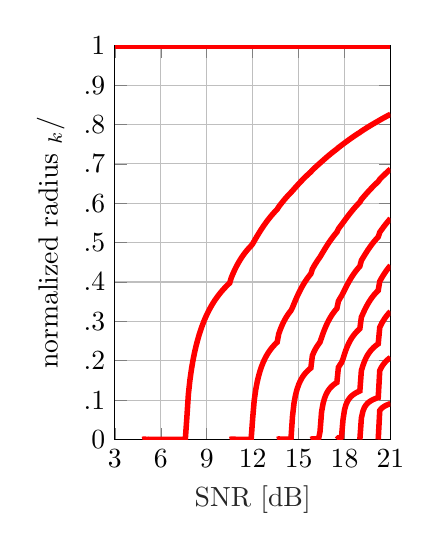
\begin{tikzpicture}

\begin{axis}[%
width=35mm,
height=50mm,
at={(0,0)},
scale only axis,
unbounded coords=jump,
xmin=3,
xmax=21,
xtick={3,6,9,12,15,18,21},
xlabel style={font=\color{white!15!black}},
xlabel={SNR [dB]},
ymin=0,
ymax=1,
ytick={0,.1,.2,.3,.4,.5,.6,.7,.8,.9,1},
yticklabels={0,.1,.2,.3,.4,.5,.6,.7,.8,.9,1},
ylabel={normalized radius $\Radius_k / \DiskRadius$},
axis background/.style={fill=white},
xmajorgrids,
ymajorgrids,
legend style={legend cell align=left, align=left, draw=white!15!black}
]
\addplot [color=red, line width=2.0pt, forget plot]
  table[row sep=crcr]{%
3	1\\
3.1	1\\
3.2	1\\
3.3	1\\
3.4	1\\
3.5	1\\
3.6	1\\
3.7	1\\
3.8	1\\
3.9	1\\
4	1\\
4.1	1\\
4.2	1\\
4.3	1\\
4.4	1\\
4.5	1\\
4.6	1\\
4.7	1\\
4.8	1\\
4.9	1\\
5	1\\
5.1	1\\
5.2	1\\
5.3	1\\
5.4	1\\
5.5	1\\
5.6	1\\
5.7	1\\
5.8	1\\
5.9	1\\
6	1\\
6.1	1\\
6.2	1\\
6.3	1\\
6.4	1\\
6.5	1\\
6.6	1\\
6.7	1\\
6.8	1\\
6.9	1\\
7	1\\
7.1	1\\
7.2	1\\
7.3	1\\
7.4	1\\
7.5	1\\
7.6	1\\
7.7	1\\
7.8	1\\
7.9	1\\
8	1\\
8.1	1\\
8.2	1\\
8.3	1\\
8.4	1\\
8.5	1\\
8.6	1\\
8.7	1\\
8.8	1\\
8.9	1\\
9	1\\
9.1	1\\
9.2	1\\
9.3	1\\
9.4	1\\
9.5	1\\
9.6	1\\
9.7	1\\
9.8	1\\
9.9	1\\
10	1\\
10.1	1\\
10.2	1\\
10.3	1\\
10.4	1\\
10.5	1\\
10.6	1\\
10.7	1\\
10.8	1\\
10.9	1\\
11	1\\
11.1	1\\
11.2	1\\
11.3	1\\
11.4	1\\
11.5	1\\
11.6	1\\
11.7	1\\
11.8	1\\
11.9	1\\
12	1\\
12.1	1\\
12.2	1\\
12.3	1\\
12.4	1\\
12.5	1\\
12.6	1\\
12.7	1\\
12.8	1\\
12.9	1\\
13	1\\
13.1	1\\
13.2	1\\
13.3	1\\
13.4	1\\
13.5	1\\
13.6	1\\
13.7	1\\
13.8	1\\
13.9	1\\
14	1\\
14.1	1\\
14.2	1\\
14.3	1\\
14.4	1\\
14.5	1\\
14.6	1\\
14.7	1\\
14.8	1\\
14.9	1\\
15	1\\
15.1	1\\
15.2	1\\
15.3	1\\
15.4	1\\
15.5	1\\
15.6	1\\
15.7	1\\
15.8	1\\
15.9	1\\
16	1\\
16.1	1\\
16.2	1\\
16.3	1\\
16.4	1\\
16.5	1\\
16.6	1\\
16.7	1\\
16.8	1\\
16.9	1\\
17	1\\
17.1	1\\
17.2	1\\
17.3	1\\
17.4	1\\
17.5	1\\
17.6	1\\
17.7	1\\
17.8	1\\
17.9	1\\
18	1\\
18.1	1\\
18.2	1\\
18.3	1\\
18.4	1\\
18.5	1\\
18.6	1\\
18.7	1\\
18.8	1\\
18.9	1\\
19	1\\
19.1	1\\
19.2	1\\
19.3	1\\
19.4	1\\
19.5	1\\
19.6	1\\
19.7	1\\
19.8	1\\
19.9	1\\
20	1\\
20.1	1\\
20.2	1\\
20.3	1\\
20.4	1\\
20.5	1\\
20.6	1\\
20.7	1\\
20.8	1\\
20.9	1\\
21	1\\
};
\addplot [color=red, line width=2.0pt, forget plot]
  table[row sep=crcr]{%
4.8	0\\
4.9	0.00108742990185637\\
5	0.000715168568966009\\
5.1	2.36227519116172e-05\\
5.2	0.000582740548106665\\
5.3	0.000117688654719785\\
5.4	4.354768841701e-05\\
5.5	4.07227550051317e-05\\
5.6	0.000215128478579955\\
5.7	0.000205327289402159\\
5.8	3.53446692264463e-05\\
5.9	1.70413348356601e-05\\
6	0.000186000331085904\\
6.1	0.000182007028711493\\
6.2	3.58439580568565e-05\\
6.3	0.00017729627136276\\
6.4	3.50100025048173e-05\\
6.5	3.51808085250818e-05\\
6.6	7.92683833954985e-05\\
6.7	1.60097160302767e-05\\
6.8	7.25429026856612e-06\\
6.9	0.000186572109911583\\
7	3.86710671470354e-05\\
7.1	0.000405164970284484\\
7.2	0.00017289048178051\\
7.3	0.000188699957254849\\
7.4	9.60216193916144e-05\\
7.5	0.000117226839503867\\
7.6	3.531288872765e-05\\
7.7	0.0549690854986438\\
7.8	0.114545838832552\\
7.9	0.150630870832004\\
8	0.178203319844855\\
8.1	0.200871965836622\\
8.2	0.220215747958138\\
8.3	0.237103894598139\\
8.4	0.252079096778632\\
8.5	0.265508708527985\\
8.6	0.277656964569554\\
8.7	0.288722112724108\\
8.8	0.298858260050282\\
8.9	0.308187718806489\\
9	0.316810524028532\\
9.1	0.324809428397061\\
9.2	0.332254017539524\\
9.3	0.339203628237407\\
9.4	0.345709702593299\\
9.5	0.351816420311785\\
9.6	0.357562834306152\\
9.7	0.362983405560455\\
9.8	0.368108770072515\\
9.9	0.372966294042916\\
10	0.377580600489562\\
10.1	0.381973780801602\\
10.2	0.38616601064915\\
10.3	0.390175668362402\\
10.4	0.394019425639315\\
10.5	0.397712682899409\\
10.6	0.410637958059668\\
10.7	0.420044198704291\\
10.8	0.428723911088846\\
10.9	0.436751279611317\\
11	0.444191708897355\\
11.1	0.451101142294171\\
11.2	0.457529081854976\\
11.3	0.463518842045414\\
11.4	0.469109030696563\\
11.5	0.474334165116755\\
11.6	0.479225181130584\\
11.7	0.483810000974801\\
11.8	0.48811357190989\\
11.9	0.492159206683057\\
12	0.497197964536963\\
12.1	0.504049373583994\\
12.2	0.510773887737557\\
12.3	0.517345176237807\\
12.4	0.52374111407988\\
12.5	0.529946477899216\\
12.6	0.535950706612465\\
12.7	0.54174663213039\\
12.8	0.547331583755147\\
12.9	0.552705709472591\\
13	0.557870968346021\\
13.1	0.562831745831625\\
13.2	0.567593591214104\\
13.3	0.572163079158298\\
13.4	0.576547512791333\\
13.5	0.580754819570623\\
13.6	0.584793191282241\\
13.7	0.591030588806071\\
13.8	0.596143632863425\\
13.9	0.601109555229906\\
14	0.605919570486281\\
14.1	0.610567736138176\\
14.2	0.615050869017847\\
14.3	0.619367301165629\\
14.4	0.623517677147674\\
14.5	0.627503227036324\\
14.6	0.631725093296361\\
14.7	0.63617676679067\\
14.8	0.640576299538078\\
14.9	0.644910538748201\\
15	0.649171387584829\\
15.1	0.653350424177298\\
15.2	0.657440435191642\\
15.3	0.661435420975396\\
15.4	0.665330660878231\\
15.5	0.669122943161098\\
15.6	0.672809366609471\\
15.7	0.67638899500079\\
15.8	0.679861177724221\\
15.9	0.684292289222839\\
16	0.688019932713109\\
16.1	0.691672894516253\\
16.2	0.695245359085815\\
16.3	0.698732374276714\\
16.4	0.702142921935423\\
16.5	0.705644406854649\\
16.6	0.709110374201047\\
16.7	0.712534929871395\\
16.8	0.715913099444947\\
16.9	0.719240572742295\\
17	0.722512588118436\\
17.1	0.725725453115251\\
17.2	0.728876220986828\\
17.3	0.73196123411213\\
17.4	0.73497818296098\\
17.5	0.737924498054913\\
17.6	0.741339317209257\\
17.7	0.744346320482694\\
17.8	0.747301127358671\\
17.9	0.75023240446243\\
18	0.753150450553281\\
18.1	0.756034190028871\\
18.2	0.758880755244656\\
18.3	0.761690133644809\\
18.4	0.764459185865054\\
18.5	0.767186051832777\\
18.6	0.769868066338849\\
18.7	0.772503304649581\\
18.8	0.775089524262916\\
18.9	0.777624908885243\\
19	0.780107716739216\\
19.1	0.782974128760185\\
19.2	0.785499301329301\\
19.3	0.78799565019596\\
19.4	0.790460871934054\\
19.5	0.792894884401883\\
19.6	0.795295858131837\\
19.7	0.797663250039088\\
19.8	0.799994909534099\\
19.9	0.802289743928268\\
20	0.804546312352308\\
20.1	0.806762699628905\\
20.2	0.808938040899097\\
20.3	0.811375308226665\\
20.4	0.813564872980925\\
20.5	0.815727223241016\\
20.6	0.817862171901808\\
20.7	0.819968594585984\\
20.8	0.822045534602101\\
20.9	0.824092547817722\\
21	0.826108041588946\\
};
\addplot [color=red, line width=2.0pt, forget plot]
  table[row sep=crcr]{%
10.5	0\\
10.6	0.000923073163269465\\
10.7	0.000618883144281569\\
10.8	0.0011574234067402\\
10.9	0.000460331138676463\\
11	0.000415420051600965\\
11.1	0.000174133344664228\\
11.2	0.00037075034240293\\
11.3	0.000160924834450618\\
11.4	0.000359438799885663\\
11.5	0.000359863360033692\\
11.6	0.000168896565955589\\
11.7	0.000414740764109663\\
11.8	0.000220174588586026\\
11.9	0.00075059575433045\\
12	0.0538996793827246\\
12.1	0.0992667643096241\\
12.2	0.126749236775295\\
12.3	0.147069302409689\\
12.4	0.163166574924379\\
12.5	0.176406416248957\\
12.6	0.187563631711046\\
12.7	0.197129296526612\\
12.8	0.205445301800387\\
12.9	0.212757586875457\\
13	0.219249737813364\\
13.1	0.225064315400113\\
13.2	0.230313482827112\\
13.3	0.2350870088107\\
13.4	0.239457628431525\\
13.5	0.243486046800225\\
13.6	0.247222170203961\\
13.7	0.267912435562323\\
13.8	0.278913467793153\\
13.9	0.288527843691166\\
14	0.296994504205396\\
14.1	0.30449988346072\\
14.2	0.311194079298154\\
14.3	0.317196639318917\\
14.4	0.322607017741237\\
14.5	0.327505211656219\\
14.6	0.335100640846293\\
14.7	0.344759463164376\\
14.8	0.354057629858766\\
14.9	0.362888951586412\\
15	0.371219954872121\\
15.1	0.379034552512755\\
15.2	0.386339433812921\\
15.3	0.393154458815079\\
15.4	0.399507854918631\\
15.5	0.405433262313741\\
15.6	0.410962413504222\\
15.7	0.416129818505247\\
15.8	0.420967457634276\\
15.9	0.43296688716648\\
16	0.439847021526236\\
16.1	0.446346307625195\\
16.2	0.452463297389828\\
16.3	0.458204825713507\\
16.4	0.463696162578998\\
16.5	0.470290399532957\\
16.6	0.476821120698258\\
16.7	0.483227716926286\\
16.8	0.489468440524674\\
16.9	0.495511285924633\\
17	0.501330953465789\\
17.1	0.506915006185896\\
17.2	0.512258713978786\\
17.3	0.517357241397997\\
17.4	0.522214661660522\\
17.5	0.526835323179665\\
17.6	0.535023152938954\\
17.7	0.540361616034112\\
17.8	0.545504879499927\\
17.9	0.550716165763387\\
18	0.556052032839144\\
18.1	0.5613152722222\\
18.2	0.566479778252446\\
18.3	0.571543065830871\\
18.4	0.576480853278836\\
18.5	0.581282365987822\\
18.6	0.585933942064311\\
18.7	0.59042947223228\\
18.8	0.594761400474814\\
18.9	0.598928624098183\\
19	0.602930138698486\\
19.1	0.609729379767579\\
19.2	0.61429037850039\\
19.3	0.618802051149629\\
19.4	0.623241996015554\\
19.5	0.62760907523295\\
19.6	0.631886246401354\\
19.7	0.636071311683925\\
19.8	0.640148970414413\\
19.9	0.644115169593847\\
20	0.647963521708323\\
20.1	0.651687448451124\\
20.2	0.65528650308097\\
20.3	0.660855830733939\\
20.4	0.664793906404949\\
20.5	0.668671225789928\\
20.6	0.672485138899848\\
20.7	0.676227101094162\\
20.8	0.679889497556996\\
20.9	0.683470246312589\\
21	0.686959071433329\\
};
\addplot [color=red, line width=2.0pt, forget plot]
  table[row sep=crcr]{%
13.6	0\\
13.7	0.00141558287062724\\
13.8	0.00120996023252675\\
13.9	0.00102498266178987\\
14	0.00083270438973438\\
14.1	0.000784001024922552\\
14.2	0.000750998125052325\\
14.3	0.000816669434928737\\
14.4	0.000948208405869488\\
14.5	0.000755359634345097\\
14.6	0.0583270010844054\\
14.7	0.0923512091252504\\
14.8	0.113082477532827\\
14.9	0.127826237921294\\
15	0.139063789184022\\
15.1	0.147979382767321\\
15.2	0.155262814507289\\
15.3	0.161351423337007\\
15.4	0.166540628065096\\
15.5	0.171039840704441\\
15.6	0.174996873911037\\
15.7	0.17852404419213\\
15.8	0.181706893911079\\
15.9	0.213139306244181\\
16	0.222258693849792\\
16.1	0.229908839061069\\
16.2	0.236419881317052\\
16.3	0.242026639815727\\
16.4	0.247474265513175\\
16.5	0.258990723419318\\
16.6	0.269977544340603\\
16.7	0.280119921526679\\
16.8	0.289336418063854\\
16.9	0.297640230540068\\
17	0.30509674034236\\
17.1	0.311803962908302\\
17.2	0.317861368677348\\
17.3	0.323347073831987\\
17.4	0.32834234735422\\
17.5	0.332911035399956\\
17.6	0.351301064655371\\
17.7	0.358268232053218\\
17.8	0.364627486960953\\
17.9	0.371766010191944\\
18	0.379736535571505\\
18.1	0.387476248320953\\
18.2	0.394864462457467\\
18.3	0.401907780329692\\
18.4	0.408534747872063\\
18.5	0.41474943680187\\
18.6	0.420546505003426\\
18.7	0.425951587131456\\
18.8	0.430980736230476\\
18.9	0.435668298297628\\
19	0.440041462931535\\
19.1	0.454718501755763\\
19.2	0.461202697507944\\
19.3	0.467609189656664\\
19.4	0.47382500458015\\
19.5	0.479854319071817\\
19.6	0.48562893648628\\
19.7	0.491160457673095\\
19.8	0.4964069737763\\
19.9	0.50138092963219\\
20	0.50608144933983\\
20.1	0.510512307432464\\
20.2	0.514692809529127\\
20.3	0.526336888574238\\
20.4	0.531834827491359\\
20.5	0.537189824690648\\
20.6	0.54239632867978\\
20.7	0.547426031564634\\
20.8	0.552256296599264\\
20.9	0.556892344554142\\
21	0.561311268548704\\
};
\addplot [color=red, line width=2.0pt, forget plot]
  table[row sep=crcr]{%
15.8	0\\
15.9	0.00182165931880792\\
16	0.0016117464566166\\
16.1	0.00168580488464605\\
16.2	0.00175932224739402\\
16.3	0.00106375676332797\\
16.4	0.0203561362958292\\
16.5	0.0703197376412677\\
16.6	0.0918304845713368\\
16.7	0.10547177141731\\
16.8	0.115094426808308\\
16.9	0.12230257958952\\
17	0.127942154736589\\
17.1	0.132519601509149\\
17.2	0.136349642161871\\
17.3	0.139625115158053\\
17.4	0.142488199693001\\
17.5	0.145032311153903\\
17.6	0.183285851659775\\
17.7	0.189741363978182\\
17.8	0.195111875857795\\
17.9	0.204739276680638\\
18	0.217347335767141\\
18.1	0.228478016173287\\
18.2	0.238004614558236\\
18.3	0.246280917216901\\
18.4	0.25339886718928\\
18.5	0.259599114222038\\
18.6	0.265024912308197\\
18.7	0.269836306012076\\
18.8	0.274130406182358\\
18.9	0.27801038473184\\
19	0.281546771398302\\
19.1	0.310822286773463\\
19.2	0.319516527791491\\
19.3	0.327945076895953\\
19.4	0.335739596793689\\
19.5	0.342991142006973\\
19.6	0.34957433715872\\
19.7	0.355615053141806\\
19.8	0.361083866399667\\
19.9	0.366077424590035\\
20	0.370641685509901\\
20.1	0.374821811530183\\
20.2	0.378679862088016\\
20.3	0.401777824987481\\
20.4	0.408672848644797\\
20.5	0.415189155579872\\
20.6	0.421349086403916\\
20.7	0.427113923912603\\
20.8	0.432459732984393\\
20.9	0.437444782581067\\
21	0.442052561655505\\
};
\addplot [color=red, line width=2.0pt, forget plot]
  table[row sep=crcr]{%
17.5	0\\
17.6	0.00394364207299766\\
17.7	0.00326997529041591\\
17.8	0.00582103735169237\\
17.9	0.0501719093991456\\
18	0.0757536807997611\\
18.1	0.0891765329803347\\
18.2	0.0976341209159847\\
18.3	0.103708933477076\\
18.4	0.108269794194932\\
18.5	0.111902307481826\\
18.6	0.114886420187694\\
18.7	0.117429176144777\\
18.8	0.119638382890491\\
18.9	0.121606345017569\\
19	0.123391092528801\\
19.1	0.175287502001684\\
19.2	0.187623860137304\\
19.3	0.198295834813794\\
19.4	0.206902639553589\\
19.5	0.214154984567676\\
19.6	0.220142378046592\\
19.7	0.22531264952175\\
19.8	0.229739346634419\\
19.9	0.233639372686721\\
20	0.237112576896494\\
20.1	0.240234173707743\\
20.2	0.243088274817109\\
20.3	0.284766591685173\\
20.4	0.292715699107343\\
20.5	0.299729266480319\\
20.6	0.306023117853983\\
20.7	0.31163473190385\\
20.8	0.316605611967998\\
20.9	0.321101490994617\\
21	0.325139070410695\\
};
\addplot [color=red, line width=2.0pt, forget plot]
  table[row sep=crcr]{%
19	0\\
19.1	0.0543986317309281\\
19.2	0.0717068254884314\\
19.3	0.0814882470258835\\
19.4	0.087546023255399\\
19.5	0.0919598091696579\\
19.6	0.0952420128881692\\
19.7	0.0979319354755496\\
19.8	0.100141350213267\\
19.9	0.102051482953941\\
20	0.103737202759292\\
20.1	0.105247539912693\\
20.2	0.106635459616399\\
20.3	0.174938674826805\\
20.4	0.182815781617275\\
20.5	0.188974602054531\\
20.6	0.194126050824037\\
20.7	0.198481965412902\\
20.8	0.202182978099286\\
20.9	0.205461226311456\\
21	0.2083553877801\\
};
\addplot [color=red, line width=2.0pt, forget plot]
  table[row sep=crcr]%
\put(-60,143){\scriptsize{$k \!=\! 1$}}%
\put(-77,78){\scriptsize{$k \!=\! 2$}}%
\put(-64,53){\scriptsize{$k \!=\! 3$}}%
\put(-44,41){\scriptsize{$...$}}%
\label{fig:Radii_evolution}%
}
\
\subfloat[circle probabilities]{%
\resizebox{!}{55mm}{% This file was created by matlab2tikz.
%
%The latest updates can be retrieved from
%  http://www.mathworks.com/matlabcentral/fileexchange/22022-matlab2tikz-matlab2tikz
%where you can also make suggestions and rate matlab2tikz.
%
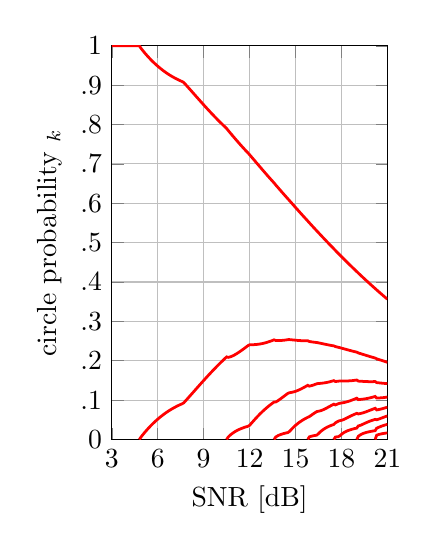
\begin{tikzpicture}

\begin{axis}[%
width=35mm,
height=50mm,
at={(0,0)},
scale only axis,
unbounded coords=jump,
xmin=3,
xmax=21,
xtick={3,6,9,12,15,18,21},
xlabel={SNR [dB]},
ymin=0,
ymax=1,
ytick={0,.1,.2,.3,.4,.5,.6,.7,.8,.9,1},
yticklabels={0,.1,.2,.3,.4,.5,.6,.7,.8,.9,1},
ylabel={circle probability $\CircProb_k$},
axis background/.style={fill=white},
xmajorgrids,
ymajorgrids,
legend style={legend cell align=left, align=left, draw=white!15!black}
]
\addplot [color=red, line width=1.0pt, forget plot]
  table[row sep=crcr]{%
3	1\\
4.8	1\\
4.9	0.994085857509207\\
5	0.989132055634811\\
5.1	0.984349673716114\\
5.2	0.979733823547703\\
5.3	0.975280773834439\\
5.4	0.970985728233969\\
5.5	0.966844599269895\\
5.6	0.962853263592147\\
5.7	0.959007748738371\\
5.8	0.955304182701924\\
5.9	0.951738727643758\\
6	0.948307729635642\\
6.1	0.945007687487728\\
6.2	0.941835122288339\\
6.3	0.938786659618329\\
6.4	0.935859161704314\\
6.5	0.933049433612488\\
6.6	0.930354471303208\\
6.7	0.927771379502665\\
6.8	0.925297342155032\\
6.9	0.922929629944373\\
7	0.920665662617436\\
7.1	0.91850281781414\\
7.2	0.91643883939068\\
7.3	0.914471233046079\\
7.4	0.912597772524836\\
7.5	0.910816262559762\\
7.6	0.909124609263932\\
7.7	0.906752491209398\\
7.8	0.902491200110124\\
7.9	0.898189164574736\\
8	0.89385384865852\\
8.1	0.889492082872415\\
8.2	0.885110890425168\\
8.3	0.880716832198228\\
8.4	0.876316154368053\\
8.5	0.87191493091916\\
8.6	0.867518860391971\\
8.7	0.863133328576262\\
8.8	0.858763263862367\\
8.9	0.854413458125616\\
9	0.850088230750172\\
9.1	0.845791546616539\\
9.2	0.841527109090658\\
9.3	0.837298249684641\\
9.4	0.833107906357325\\
9.5	0.828958871002651\\
9.6	0.824853533830862\\
9.7	0.820794017897418\\
9.8	0.81678216669955\\
9.9	0.812819659538965\\
10	0.808907740661317\\
10.1	0.80504771520665\\
10.2	0.801240414495478\\
10.3	0.797486562240611\\
10.4	0.793786778958904\\
10.5	0.790141402873227\\
10.6	0.785083547777089\\
10.7	0.780431725120599\\
10.8	0.775799890349058\\
10.9	0.771194162702737\\
11	0.766620129434578\\
11.1	0.762083186911573\\
11.2	0.757588255092395\\
11.3	0.753140015631012\\
11.4	0.748742716464239\\
11.5	0.744400308172314\\
11.6	0.740116320768605\\
11.7	0.735893984869181\\
11.8	0.731736291194374\\
11.9	0.727645721171727\\
12	0.723415028398099\\
12.1	0.718863279504446\\
12.2	0.714300497513231\\
12.3	0.709731065446174\\
12.4	0.705159617052783\\
12.5	0.700590522416287\\
12.6	0.696028118625306\\
12.7	0.69147672924573\\
12.8	0.686940483767266\\
12.9	0.682423284022774\\
13	0.677928971526873\\
13.1	0.673461109205631\\
13.2	0.669023101291096\\
13.3	0.664618149958045\\
13.4	0.66024918449984\\
13.5	0.655919041247411\\
13.6	0.651630145792523\\
13.7	0.646923575522504\\
13.8	0.642408574502066\\
13.9	0.637907210270159\\
14	0.633423598295479\\
14.1	0.628961710257904\\
14.2	0.624525393651876\\
14.3	0.620118556185568\\
14.4	0.615744811910472\\
14.5	0.611407895111781\\
14.6	0.607034623722858\\
14.7	0.602616699040741\\
14.8	0.59820518485\\
14.9	0.593802940910421\\
15	0.589412132351276\\
15.1	0.58503524310378\\
15.2	0.580674769000019\\
15.3	0.576333368398723\\
15.4	0.572013552973276\\
15.5	0.567717812826103\\
15.6	0.563448817139363\\
15.7	0.559208876608805\\
15.8	0.555000404440569\\
15.9	0.550589819508059\\
16	0.546329285973088\\
16.1	0.542087716592573\\
16.2	0.537867496667975\\
16.3	0.533671094391717\\
16.4	0.529498393359138\\
16.5	0.525316049824043\\
16.6	0.521147470848312\\
16.7	0.516994088764049\\
16.8	0.512857266155298\\
16.9	0.508738273575719\\
17	0.504638821877251\\
17.1	0.500560375762574\\
17.2	0.496504398134553\\
17.3	0.492472675346512\\
17.4	0.488466835155232\\
17.5	0.48448869956222\\
17.6	0.480410047975778\\
17.7	0.476434299918982\\
17.8	0.472480617326786\\
17.9	0.468543770569587\\
18	0.464621291767987\\
18.1	0.460717574467965\\
18.2	0.456833543131586\\
18.3	0.452969469594352\\
18.4	0.4491263574374\\
18.5	0.445305008911254\\
18.6	0.441506514372574\\
18.7	0.437731998033998\\
18.8	0.433982462823441\\
18.9	0.43025908141316\\
19	0.426563134248308\\
19.1	0.422779909168014\\
19.2	0.419097079227011\\
19.3	0.415434637823051\\
19.4	0.411793559401216\\
19.5	0.408173895567415\\
19.6	0.404576218323947\\
19.7	0.401001008045177\\
19.8	0.39744910213737\\
19.9	0.393921028391603\\
20	0.390417582782651\\
20.1	0.386939755851191\\
20.2	0.383488089670497\\
20.3	0.379980175733036\\
20.4	0.376552834749719\\
20.5	0.373147540869353\\
20.6	0.369764492731447\\
20.7	0.366404208948985\\
20.8	0.363066959725669\\
20.9	0.359753214155292\\
21	0.3564634561648\\
};
\addplot [color=red, line width=1.0pt, forget plot]
  table[row sep=crcr]{%
4.8	0\\
4.9	0.00591414249079317\\
5	0.0108679443651893\\
5.1	0.015650326283886\\
5.2	0.0202661764522967\\
5.3	0.0247192261655612\\
5.4	0.0290142717660311\\
5.5	0.0331554007301052\\
5.6	0.0371467364078531\\
5.7	0.0409922512616291\\
5.8	0.0446958172980758\\
5.9	0.0482612723562416\\
6	0.0516922703643575\\
6.1	0.0549923125122725\\
6.2	0.0581648777116607\\
6.3	0.0612133403816713\\
6.4	0.0641408382956861\\
6.5	0.0669505663875125\\
6.6	0.0696455286967924\\
6.7	0.072228620497335\\
6.8	0.0747026578449677\\
6.9	0.0770703700556275\\
7	0.0793343373825637\\
7.1	0.0814971821858598\\
7.2	0.0835611606093196\\
7.3	0.0855287669539214\\
7.4	0.0874022274751639\\
7.5	0.0891837374402381\\
7.6	0.090875390736068\\
7.7	0.0932475087906018\\
7.8	0.0975087998898757\\
7.9	0.101810835425264\\
8	0.10614615134148\\
8.1	0.110507917127585\\
8.2	0.114889109574832\\
8.3	0.119283167801772\\
8.4	0.123683845631947\\
8.5	0.128085069080841\\
8.6	0.132481139608029\\
8.7	0.136866671423738\\
8.8	0.141236736137633\\
8.9	0.145586541874384\\
9	0.149911769249828\\
9.1	0.154208453383461\\
9.2	0.158472890909342\\
9.3	0.162701750315359\\
9.4	0.166892093642675\\
9.5	0.171041128997349\\
9.6	0.175146466169138\\
9.7	0.179205982102582\\
9.8	0.18321783330045\\
9.9	0.187180340461035\\
10	0.191092259338683\\
10.1	0.194952284793351\\
10.2	0.198759585504522\\
10.3	0.202513437759389\\
10.4	0.206213221041096\\
10.5	0.209858597126773\\
10.6	0.208690416140647\\
10.7	0.209544461383912\\
10.8	0.210856551619155\\
10.9	0.212534718564383\\
11	0.214505574451963\\
11.1	0.216711647852734\\
11.2	0.219106273719628\\
11.3	0.221651540920499\\
11.4	0.224315989078333\\
11.5	0.227073550563973\\
11.6	0.229902371388309\\
11.7	0.232783874248066\\
11.8	0.235702540464575\\
11.9	0.238644772350827\\
12	0.240521847319539\\
12.1	0.240667267720652\\
12.2	0.24081723076268\\
12.3	0.241012386705513\\
12.4	0.241285521083002\\
12.5	0.241658744323528\\
12.6	0.242146324451877\\
12.7	0.242756722844301\\
12.8	0.243491624752972\\
12.9	0.244348992552272\\
13	0.245324015525645\\
13.1	0.246409311493789\\
13.2	0.247596188581523\\
13.3	0.248875168439049\\
13.4	0.250236523182877\\
13.5	0.251670088662818\\
13.6	0.253166263881957\\
13.7	0.251632717121978\\
13.8	0.251494213508184\\
13.9	0.25145566516308\\
14	0.251529233788657\\
14.1	0.251721970145919\\
14.2	0.252036116562207\\
14.3	0.252471083646932\\
14.4	0.253023039842213\\
14.5	0.253686948842663\\
14.6	0.253817804930899\\
14.7	0.253451618782633\\
14.8	0.253051797868226\\
14.9	0.252644158956415\\
15	0.252245684632386\\
15.1	0.251873583835286\\
15.2	0.251542056497814\\
15.3	0.251262609829986\\
15.4	0.251043996209329\\
15.5	0.250891903723002\\
15.6	0.250810782314701\\
15.7	0.250801985942372\\
15.8	0.250865735797684\\
15.9	0.249007730599352\\
16	0.248376472979845\\
16.1	0.247781600085316\\
16.2	0.247235470398556\\
16.3	0.246748251041932\\
16.4	0.24629974382994\\
16.5	0.24553500587747\\
16.6	0.244733005457586\\
16.7	0.24390913472761\\
16.8	0.24307631394293\\
16.9	0.242246376773067\\
17	0.241431242553555\\
17.1	0.240640509802662\\
17.2	0.23988201717176\\
17.3	0.239164344642736\\
17.4	0.238493261856631\\
17.5	0.23787435395742\\
17.6	0.23607998506316\\
17.7	0.235126833912192\\
17.8	0.234196263535567\\
17.9	0.23321623938345\\
18	0.232164442071271\\
18.1	0.231096770404051\\
18.2	0.230022084208464\\
18.3	0.228942493776107\\
18.4	0.22786759203117\\
18.5	0.22680368398499\\
18.6	0.225758696453643\\
18.7	0.224738489172555\\
18.8	0.223750012332662\\
18.9	0.222798197026333\\
19	0.221888033612889\\
19.1	0.219900982224781\\
19.2	0.21870671600168\\
19.3	0.217500104931213\\
19.4	0.21628938738559\\
19.5	0.215075913001711\\
19.6	0.21386677037751\\
19.7	0.212664589446997\\
19.8	0.211476681555106\\
19.9	0.21030733011409\\
20	0.209161524125983\\
20.1	0.20804516579774\\
20.2	0.206961554756945\\
20.3	0.205056813894727\\
20.4	0.203776265185259\\
20.5	0.202495498706706\\
20.6	0.201216632555265\\
20.7	0.199943967686046\\
20.8	0.198681833866327\\
20.9	0.197432463263473\\
21	0.196202016246899\\
};
\addplot [color=red, line width=1.0pt, forget plot]
  table[row sep=crcr]{%
10.5	0\\
10.6	0.00622603608226431\\
10.7	0.0100238134954888\\
10.8	0.0133435580317879\\
10.9	0.0162711187328798\\
11	0.0188742961134586\\
11.1	0.0212051652356924\\
11.2	0.0233054711879769\\
11.3	0.0252084434484888\\
11.4	0.026941294457428\\
11.5	0.0285261412637135\\
11.6	0.0299813078430856\\
11.7	0.0313221408827529\\
11.8	0.0325611683410505\\
11.9	0.0337095064774462\\
12	0.0360631242823618\\
12.1	0.0404694527749023\\
12.2	0.0448822717240895\\
12.3	0.0492565478483135\\
12.4	0.0535548618642153\\
12.5	0.0577507332601845\\
12.6	0.0618255569228171\\
12.7	0.0657665479099684\\
12.8	0.0695678914797616\\
12.9	0.0732277234249543\\
13	0.076747012947482\\
13.1	0.0801295793005806\\
13.2	0.0833807101273814\\
13.3	0.0865066816029057\\
13.4	0.0895142923172835\\
13.5	0.0924108700897719\\
13.6	0.0952035903255206\\
13.7	0.0952439575642316\\
13.8	0.0974220975502719\\
13.9	0.0999712043377028\\
14	0.102737365321882\\
14.1	0.105619734735191\\
14.2	0.108550744605521\\
14.3	0.111484187847514\\
14.4	0.114389046124542\\
14.5	0.117244146142978\\
14.6	0.11879839774349\\
14.7	0.119442673914126\\
14.8	0.120223785050796\\
14.9	0.121216279036315\\
15	0.122437244704599\\
15.1	0.123879599611189\\
15.2	0.125518384862558\\
15.3	0.127321112684625\\
15.4	0.129253411374006\\
15.5	0.131282399880822\\
15.6	0.133379108041175\\
15.7	0.13551859344427\\
15.8	0.137679415118713\\
15.9	0.135521411218406\\
16	0.136449018702236\\
16.1	0.137567283141683\\
16.2	0.138858625544419\\
16.3	0.140300572184245\\
16.4	0.141774828079013\\
16.5	0.142196912773651\\
16.6	0.142576141867706\\
16.7	0.142975790639794\\
16.8	0.143437246433009\\
16.9	0.143990594447486\\
17	0.144654002977522\\
17.1	0.145431772648536\\
17.2	0.146320378537264\\
17.3	0.14731427231403\\
17.4	0.148401225450933\\
17.5	0.149568901765668\\
17.6	0.147347036837911\\
17.7	0.14774028114771\\
17.8	0.148237891369699\\
17.9	0.148526618362574\\
18	0.148560497201473\\
18.1	0.14857943977813\\
18.2	0.148617363500859\\
18.3	0.148680443897244\\
18.4	0.148798036172801\\
18.5	0.148981263118509\\
18.6	0.149243036363789\\
18.7	0.149586097455773\\
18.8	0.15001406611392\\
18.9	0.150522184628426\\
19	0.151105808997229\\
19.1	0.148369666539907\\
19.2	0.148150157354291\\
19.3	0.147902425878173\\
19.4	0.147660865211137\\
19.5	0.147428343145285\\
19.6	0.147231082756149\\
19.7	0.147071310744736\\
19.8	0.146970334267956\\
19.9	0.146930548313084\\
20	0.146958616468542\\
20.1	0.147058573503706\\
20.2	0.147227709351306\\
20.3	0.144602254102466\\
20.4	0.144164273289576\\
20.5	0.14373489252238\\
20.6	0.143318944676414\\
20.7	0.142930489791075\\
20.8	0.142581799013672\\
20.9	0.14227585750159\\
21	0.142026694907654\\
};
\addplot [color=red, line width=1.0pt, forget plot]
  table[row sep=crcr]{%
13.6	0\\
13.7	0.00619974979128671\\
13.8	0.00867511443947805\\
13.9	0.0106659202290578\\
14	0.0123098025939824\\
14.1	0.0136965848609857\\
14.2	0.0148877451803965\\
14.3	0.0159261723199854\\
14.4	0.0168431021227732\\
14.5	0.0176610099025792\\
14.6	0.0203491736027536\\
14.7	0.0244890082625005\\
14.8	0.0285192322309776\\
14.9	0.0323366210968487\\
15	0.0359049383117385\\
15.1	0.0392115734497452\\
15.2	0.0422647896396086\\
15.3	0.0450829090866661\\
15.4	0.0476890394433889\\
15.5	0.0501078835700741\\
15.6	0.0523612925047608\\
15.7	0.0544705440045532\\
15.8	0.0564544446430336\\
15.9	0.0581606773633244\\
16	0.0608542352139238\\
16.1	0.0635715886532671\\
16.2	0.0662289988019236\\
16.3	0.0687851440679686\\
16.4	0.0710884197887321\\
16.5	0.0718188747547243\\
16.6	0.0727403985243879\\
16.7	0.0739856994985615\\
16.8	0.0755441156625838\\
16.9	0.0773519880161659\\
17	0.0793296862977932\\
17.1	0.0814056835054632\\
17.2	0.0835243579863754\\
17.3	0.085645018948476\\
17.4	0.0877390597234794\\
17.5	0.0897874340683352\\
17.6	0.0877900062859327\\
17.7	0.089355435055888\\
17.8	0.0910580010105438\\
17.9	0.0921695366654812\\
18	0.0927597737718901\\
18.1	0.0934236821075096\\
18.2	0.0942344495475713\\
18.3	0.0951854394613619\\
18.4	0.0962964928799215\\
18.5	0.0975421993060033\\
18.6	0.0989020172990121\\
18.7	0.100343077537413\\
18.8	0.101840686185834\\
18.9	0.103367677143444\\
19	0.104903801001886\\
19.1	0.101336175275471\\
19.2	0.101732780762266\\
19.3	0.102111382107451\\
19.4	0.102563122013005\\
19.5	0.103082329401351\\
19.6	0.103714915316171\\
19.7	0.104442448617261\\
19.8	0.105280048304195\\
19.9	0.106205449225913\\
20	0.107206620142617\\
20.1	0.108267891531661\\
20.2	0.109369273444608\\
20.3	0.105295289099218\\
20.4	0.105455857136396\\
20.5	0.105672441094574\\
20.6	0.105947446439764\\
20.7	0.106299828381131\\
20.8	0.106744399747788\\
20.9	0.107267443258109\\
21	0.107876364559057\\
};
\addplot [color=red, line width=1.0pt, forget plot]
  table[row sep=crcr]{%
15.8	0\\
15.9	0.00672036131085871\\
16	0.0079909871309078\\
16.1	0.00899181152716034\\
16.2	0.00980940858712726\\
16.3	0.0104949383141375\\
16.4	0.0113386149431769\\
16.5	0.0151331567701118\\
16.6	0.0188029833020088\\
16.7	0.0221352863699852\\
16.8	0.0250850578061795\\
16.9	0.027672767187562\\
17	0.0299462462938787\\
17.1	0.0319616582807643\\
17.2	0.0337688481700477\\
17.3	0.035403688748245\\
17.4	0.0368996178137249\\
17.5	0.0382806106463571\\
17.6	0.0422091544087684\\
17.7	0.0445452489731583\\
17.8	0.046701879603102\\
17.9	0.0479378806754042\\
18	0.0487928355789137\\
18.1	0.0500990829091574\\
18.2	0.0517777407982094\\
18.3	0.0536654828751182\\
18.4	0.0556441510063992\\
18.5	0.0576271928472693\\
18.6	0.0595629941525393\\
18.7	0.0614250604001642\\
18.8	0.0631999545793128\\
18.9	0.0648862849126405\\
19	0.0664852617387241\\
19.1	0.0649901893626543\\
19.2	0.0657530520255664\\
19.3	0.0666168617097408\\
19.4	0.0676993304817311\\
19.5	0.0689411735432457\\
19.6	0.0703365809897503\\
19.7	0.0718124369391259\\
19.8	0.073339176049933\\
19.9	0.0748737420358908\\
20	0.0763909693362787\\
20.1	0.0778735911970273\\
20.2	0.0793095663414384\\
20.3	0.0751567299620149\\
20.4	0.0758376517693522\\
20.5	0.0766614793661144\\
20.6	0.0775959714166009\\
20.7	0.078633144969019\\
20.8	0.0797605175825132\\
20.9	0.0809364048260797\\
21	0.0821454585774737\\
};
\addplot [color=red, line width=1.0pt, forget plot]
  table[row sep=crcr]{%
17.5	0\\
17.6	0.00616376942844972\\
17.7	0.00679790099207047\\
17.8	0.00732534715430257\\
17.9	0.00960595434350261\\
18	0.0131011596084653\\
18.1	0.0160834503331861\\
18.2	0.0185148188133102\\
18.3	0.0205566703958169\\
18.4	0.0222673704723093\\
18.5	0.0237406518319748\\
18.6	0.025026741358443\\
18.7	0.0261752774000973\\
18.8	0.0272128179648298\\
18.9	0.028166574875996\\
19	0.0290539604009646\\
19.1	0.0344486275663355\\
19.2	0.0355497880771422\\
19.3	0.037089982653807\\
19.4	0.0388722906239355\\
19.5	0.0407188535277312\\
19.6	0.0425128886020971\\
19.7	0.0442211997311357\\
19.8	0.0458130816694544\\
19.9	0.0472972912937967\\
20	0.0486787746698649\\
20.1	0.049965875718693\\
20.2	0.0511727538411291\\
20.3	0.050154917419502\\
20.4	0.0513733659965498\\
20.5	0.0527648433279035\\
20.6	0.0542264049189918\\
20.7	0.0557052438703645\\
20.8	0.057162629112978\\
20.9	0.0585734506430372\\
21	0.0599212127523752\\
};
\addplot [color=red, line width=1.0pt, forget plot]
  table[row sep=crcr]{%
19	0\\
19.1	0.00817444986283799\\
19.2	0.011010426552044\\
19.3	0.0133446048965633\\
19.4	0.0151214448833854\\
19.5	0.0165794918132617\\
19.6	0.0177615436343759\\
19.7	0.0187870064755665\\
19.8	0.0196715760159861\\
19.9	0.020464610625622\\
20	0.0211859124740639\\
20.1	0.0218491463999816\\
20.2	0.0224710525940772\\
20.3	0.0287388534772191\\
20.4	0.0304522453122732\\
20.5	0.0320940429805066\\
20.6	0.0336266226770359\\
20.7	0.0350315785480674\\
20.8	0.0363038325450486\\
20.9	0.0374769424456324\\
21	0.0385502435236807\\
};
\addplot [color=red, line width=1.0pt, forget plot]
  table[row sep=crcr]%
\put(-48,118){\footnotesize{$\CircProb_1$}}%
\put(-64,53){\scriptsize{$\CircProb_2$}}%
\put(-48,39){\scriptsize{$\CircProb_3$}}%
\put(-37,32){\scriptsize{$...$}}%
\label{fig:PMF_evolution}%
}
\caption{Evolution of the radii and probabilities of the circles that describe the capacity-achieving transmit distribution.}
\label{fig:Radii_PMF_evolution}
\end{figure}

\begin{figure}[t]
\centering
%\includegraphics[width=.92\columnwidth]{Rates_CapacityResults-crop}
\resizebox{.96\columnwidth}{!}{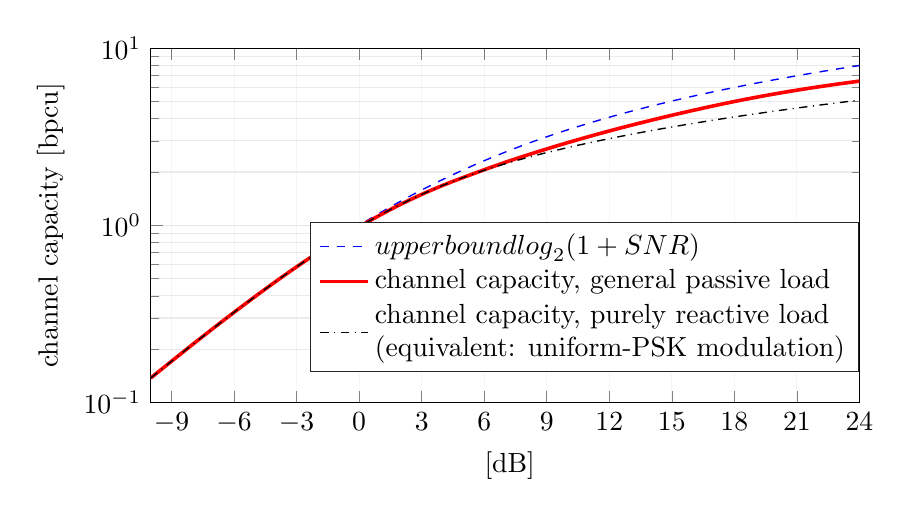
\begin{tikzpicture}

\begin{axis}[%
width=90mm,
height=45mm,
at={(0,0)},
scale only axis,
xmin=-10,
xmax=24,
xtick={ -9, -6, -3, 0, 3, 6, 9, 12, 15, 18, 21, 24},
%xticklabels={-6, -3, 0, 3, 6, 9, 12, 15, 18, 21, 24, 27},
xlabel style={font=\color{white!15!black}},
xlabel={$\SNR$ $[\mathrm{dB}]$},
ymode=log,
ymin=0.1,
ymax=10,
yminorticks=true,
ylabel style={font=\color{white!15!black}},
ylabel={channel capacity [bpcu]},
axis background/.style={fill=white},
xmajorgrids,
ymajorgrids,
yminorgrids,
grid style={opacity=0.13},
minor grid style={opacity=0.3},
label style={font=\normalsize},
legend style={at={(1,0.085)}, anchor=south east, legend cell align=left, align=left, draw=white!15!black}
]
\addplot [color=blue, dashed, line width=0.5pt]
  table[row sep=crcr]{%
-10	0.137503523749935\\
-9.5	0.153418636061023\\
-9	0.171069138514398\\
-8.5	0.190619606352057\\
-8	0.212244743260395\\
-7.5	0.236128803353125\\
-7	0.262464707140878\\
-6.5	0.291452814285687\\
-6	0.323299322693842\\
-5.5	0.358214274110159\\
-5	0.396409161163114\\
-4.5	0.438094149757986\\
-4	0.48347495334568\\
-3.5	0.532749420867551\\
-3	0.586103926445348\\
-2.5	0.643709673944082\\
-2	0.705719050773513\\
-1.5	0.772262179969205\\
-1	0.843443825203652\\
-0.5	0.91934079807483\\
0	1\\
0.5	1.0854372028192\\
1	1.17563663469239\\
1.5	1.27055139420231\\
2	1.37010466975099\\
2.5	1.47419169766592\\
3	1.58268235491156\\
3.5	1.69542425407813\\
4	1.81224619130063\\
4.5	1.9329617924573\\
5	2.0573732086068\\
5.5	2.18527472629821\\
6	2.31645617962626\\
6.5	2.45070607596247\\
7	2.58781437356203\\
7.5	2.72757487451865\\
8	2.86978721917029\\
8.5	3.01425848700632\\
9	3.16080442391302\\
9.5	3.30925032620402\\
10	3.4594316186373\\
10.5	3.61119416705619\\
11	3.76439436704286\\
11.5	3.91889904869198\\
12	4.07458523490543\\
12.5	4.23133978700232\\
13	4.38905896736305\\
13.5	4.54764794461157\\
14	4.70702026272884\\
14.5	4.86709729164214\\
15	5.02780767335052\\
15.5	5.18908677457204\\
16	5.3508761542486\\
16.5	5.51312305200527\\
17	5.67577990180488\\
17.5	5.83880387352813\\
18	6.00215644400198\\
18.5	6.16580299805362\\
19	6.32971245944191\\
19.5	6.49385695097752\\
20	6.65821148275179\\
20.5	6.82275366712554\\
21	6.98746345895592\\
21.5	7.1523229194428\\
22	7.31731600193655\\
22.5	7.48242835805457\\
23	7.64764716249041\\
23.5	7.81296095495953\\
24	7.97835949780125\\
};
\addlegendentry{$\text{upper bound log}_\text{2}\text{(1 + SNR)}$}

\addplot [color=red, line width=1.3pt]
  table[row sep=crcr]{%
-10	0.137490906666417\\
-9.5	0.153399403990599\\
-9	0.171039935249776\\
-8.5	0.190575444753509\\
-8	0.212178257195243\\
-7.5	0.236029182897772\\
-7	0.262316197838123\\
-6.5	0.291232624383457\\
-6	0.322974738129779\\
-5.5	0.357738730230072\\
-5	0.395716964847275\\
-4.5	0.43709348985187\\
-4	0.48203878775833\\
-3.5	0.530703795313945\\
-3	0.583213275981814\\
-2.5	0.639658700930992\\
-2	0.700090880847482\\
-1.5	0.764512690550033\\
-1	0.832872335579065\\
-0.5	0.905057715083341\\
0	0.980892523998895\\
0.5	1.06013479000486\\
1	1.14247853280152\\
1.5	1.22755913836571\\
2	1.31496283468871\\
2.5	1.404240323024\\
3	1.49492416330459\\
3.5	1.58654896613884\\
4	1.67867287507681\\
4.5	1.77089833749213\\
5	1.86336708293004\\
5.5	1.95951129500193\\
6	2.05944392499972\\
6.5	2.16227922545915\\
7	2.26702644878706\\
7.5	2.37263814538457\\
8	2.47879831992885\\
8.5	2.58745529907544\\
9	2.69871645260338\\
9.5	2.81240690699709\\
10	2.92808134803176\\
10.5	3.0452964353854\\
11	3.16430965375948\\
11.5	3.2854181526281\\
12	3.40818887394725\\
12.5	3.53259192319178\\
13	3.65883219897967\\
13.5	3.78674553931811\\
14	3.91623260483693\\
14.5	4.04733161815581\\
15	4.17992003073123\\
15.5	4.31401399928841\\
16	4.44948247348643\\
16.5	4.5860705935919\\
17	4.72339744708351\\
17.5	4.86097776801742\\
18	4.99826548372716\\
18.5	5.13471323627153\\
19	5.26983776127836\\
19.5	5.40327367267533\\
20	5.53479284393184\\
20.5	5.66428043683202\\
21	5.79169176380879\\
21.5	5.91702209959332\\
22	6.04029376930273\\
22.5	6.16154963982862\\
23	6.28084773802992\\
23.5	6.39825660758257\\
24	6.51385156163464\\
};
%\addlegendentry{channel capacity for arbitrary passive load}
\addlegendentry{channel capacity, general passive load}

\addplot [color=black, dashdotted, line width=0.5pt]
  table[row sep=crcr]{%
-10	0.137490906666417\\
-9.5	0.153399403990599\\
-9	0.171039935249776\\
-8.5	0.190575444753509\\
-8	0.212178257195243\\
-7.5	0.236029182897772\\
-7	0.262316197838123\\
-6.5	0.291232624383457\\
-6	0.322974738129779\\
-5.5	0.357738730230072\\
-5	0.395716964847275\\
-4.5	0.43709348985187\\
-4	0.48203878775833\\
-3.5	0.530703795313945\\
-3	0.583213275981814\\
-2.5	0.639658700930992\\
-2	0.700090880847482\\
-1.5	0.764512690550033\\
-1	0.832872335579065\\
-0.5	0.905057715083341\\
0	0.980892523998895\\
0.5	1.06013479000486\\
1	1.14247853280152\\
1.5	1.22755913836571\\
2	1.31496283468871\\
2.5	1.404240323024\\
3	1.49492416330459\\
3.5	1.58654896613884\\
4	1.67867287507681\\
4.5	1.77089833749213\\
5	1.86288989247773\\
5.5	1.95438678032001\\
6	2.04520868673105\\
6.5	2.13525386861277\\
7	2.22449012886201\\
7.5	2.3129403489088\\
8	2.40066521289591\\
8.5	2.48774607413584\\
9	2.57427050396812\\
9.5	2.66032206006254\\
10	2.74597457231891\\
10.5	2.83129019850657\\
11	2.91631995217247\\
11.5	3.00110540225082\\
12	3.08568060483823\\
12.5	3.17007378252874\\
13	3.25430861502594\\
13.5	3.3384051836574\\
14	3.42238066188835\\
14.5	3.50624983219313\\
15	3.59002548434695\\
15.5	3.67371873004793\\
16	3.75733925624968\\
16.5	3.84089553217357\\
17	3.92439498047657\\
17.5	4.00784412016336\\
18	4.09124868688507\\
18.5	4.17461373491025\\
19	4.25794372408082\\
19.5	4.34124259434809\\
20	4.42451382995459\\
20.5	4.50776051491685\\
21	4.59098538115687\\
21.5	4.67419085038305\\
22	4.7573790706311\\
22.5	4.84055194822161\\
23	4.92371117576761\\
23.5	5.00685825676705\\
24	5.08999452723369\\
};
\addlegendentry{channel capacity, purely reactive load\\(equivalent: uniform-PSK modulation)}
\end{axis}

\end{tikzpicture}%}%
\caption{Channel capacity in bit per channel use (bpcu) plotted versus $\SNR$.} % ... could be attained by error-correcting codes ... sampled from ... with infinite block length
\label{fig:Rates_Capacity}
\end{figure}

\Cref{fig:Rates_Capacity} plots $\Rate$ versus $\SNR$ for different assumptions:
\begin{itemize}
\item \textbf{The capacity-achieving $K$ and $\Radius_k$, $\CircProb_k$ are used:} At high SNR, the additional circles inside the disk ensure that the transmit signal space is utilized thoroughly. %(cf. sphere packing).
This is achieved by purposefully raising the load resistance $\Re(z) \geq 0$.
\item \textbf{Only $K = 1$ is used:} This uniform-PSK $i \sim \calU(\calC_1)$ at the disk boundary is associated with a purely reactive load ($z = jx$), which is an interesting feature from a circuit perspective. The resulting information rate also constitutes the channel capacity of reactive load modulation. At high SNR, it lacks behind general passive load modulation, because the disk interior is not utilized.
\end{itemize}
For $\SNR < 4.8\dB$ the two cases coincide precisely, because then $K=1$ achieves capacity.
%the optimal number of circles $K$ is used and 2.) $K = 1$ is enforced, e.g. for technical reasons. 
%The second case uses just the largest circle with radius $\Radius_1$ (and $\CircProb_1 = 1$), hence no optimization must be conducted. In communications-engineering terms, this corresponds to $\infty$-PSK modulation. This case is attractive from a circuit perspective because it can be realized with a purely reactive load, i.e. $\Re(z) = 0$.

\subsection{Capacity-Achieving Load Impedance Statistics}
\label{sec:loadstats}

Herein we characterize the capacity-achieving distribution of the load impedance $z$, which follows from $z = \ChannelFunc^{-1}(i)$ together with the statistics of $i$ described in \Cref{sec:CurrentStats}.

The circle $\calC_1$ maps to the imaginary axis $j\bbR = \ChannelFunc^{-1}(\calC_1)$, i.e. to the set of purely reactive loads.
In detail, $i = \DiskRadius + \DiskRadius\, e^{j\phi}$ maps to $z = jx$ with
$x = -\tan(\phi / 2)$ and $\phi \sim \calU(-\pi,\pi)$. We find that $x$ has standard Cauchy distribution; the PDF is
% with location parameter $0$ and scale parameter $1$.
%In other words, the PDF is the simple Lorentzian function
\begin{align}
f_x(x) &= \f{1}{\pi(1 + x^2)} \, , &
x &\in \bbR \, . &
%z &= jx \, ,
\label{eq:Lorentz}
\end{align}
%which is shown in \Cref{fig:Lorentz}.
This is a complete description of the capacity-achieving load statistics in the low-SNR case (where $K = 1$ is optimal) or when a purely reactive load is enforced for technical reasons. The specific probability density evolution from \Cref{eq:Lorentz} can also seen along the imaginary axis in \Cref{fig:CapAchievingDistr_z}.

%\begin{figure}[!ht]
%\centering
%\resizebox{.7\columnwidth}{!}{% This file was created by matlab2tikz.
%
%The latest updates can be retrieved from
%  http://www.mathworks.com/matlabcentral/fileexchange/22022-matlab2tikz-matlab2tikz
%where you can also make suggestions and rate matlab2tikz.
%
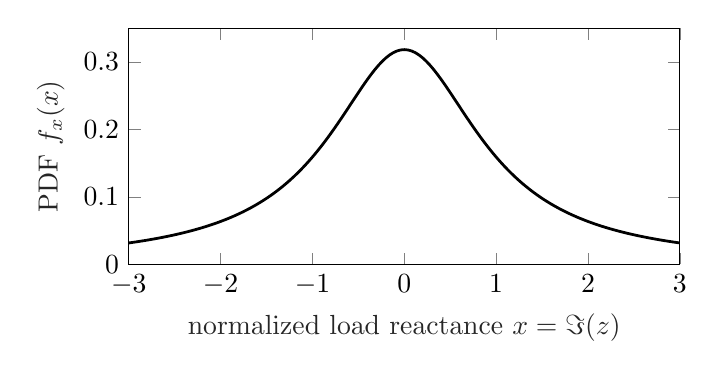
\begin{tikzpicture}

\begin{axis}[%
width=70mm,
height=30mm,
at={(0,0)},
scale only axis,
xmin=-3,
xmax=3,
%xtick={1, 2, 3, 4, 5, 6, 7, 8},
xlabel style={font=\color{white!15!black}},
xlabel={normalized load reactance $x = \Im(z)$}, %  = \f{\Im(Z\L)}{R\Tx}
ymin=0,
ymax=0.35,
ylabel style={font=\color{white!15!black}},
ylabel={PDF $f_x(x)$},
axis background/.style={fill=white},
legend style={legend cell align=left, align=left, draw=white!15!black}
]
\addplot [color=black, line width=1.0pt, forget plot]
  table[row sep=crcr]{%
-3	0.0318309886183791\\
-2.96	0.032608372211911\\
-2.92	0.0334134495910093\\
-2.88	0.0342474916276242\\
-2.84	0.0351118388395463\\
-2.8	0.0360079056768994\\
-2.76	0.036937185084454\\
-2.72	0.0379012533558524\\
-2.68	0.03890177529622\\
-2.64	0.0399405097098713\\
-2.6	0.0410193152298699\\
-2.56	0.0421401565060091\\
-2.52	0.0433051107672767\\
-2.48	0.0445163747739694\\
-2.44	0.0457762721732327\\
-2.4	0.0470872612697915\\
-2.36	0.0484519432208644\\
-2.32	0.0498730706605338\\
-2.28	0.0513535567539673\\
-2.24	0.0528964846755834\\
-2.2	0.0545051174972244\\
-2.16	0.0561829084622618\\
-2.12	0.0579335116088728\\
-2.08	0.0597607926899577\\
-2.04	0.0616688403176904\\
-2	0.0636619772367581\\
-1.96	0.0657447716010804\\
-1.92	0.0679220480931612\\
-1.88	0.0701988986820286\\
-1.84	0.0725806927635422\\
-1.8	0.0750730863641016\\
-1.76	0.0776820300136155\\
-1.72	0.0804137748039083\\
-1.68	0.0832748760422223\\
-1.64	0.0862721937835513\\
-1.6	0.0894128893774693\\
-1.56	0.0927044169920173\\
-1.52	0.0961545088762055\\
-1.48	0.0997711528911079\\
-1.44	0.103562560575153\\
-1.4	0.10753712371074\\
-1.36	0.111703357026878\\
-1.32	0.116069824308558\\
-1.28	0.120645044793735\\
-1.24	0.125437376333461\\
-1.2	0.130454871386799\\
-1.16	0.135705101544931\\
-1.12	0.141194945965131\\
-1.08	0.146930338895767\\
-1.04	0.152915971456471\\
-1	0.159154943091895\\
-0.96	0.165648358755095\\
-0.92	0.172394869033682\\
-0.88	0.179390152267691\\
-0.84	0.186626340398564\\
-0.8	0.194091394014507\\
-0.76	0.201768436982626\\
-0.72	0.209635067297017\\
-0.68	0.217662668342308\\
-0.64	0.225815753535606\\
-0.6	0.234051386899846\\
-0.56	0.242318731869512\\
-0.52	0.250558789502354\\
-0.48	0.258704393842483\\
-0.44	0.266680534671406\\
-0.4	0.274405074296371\\
-0.36	0.28178991340633\\
-0.32	0.288742639861929\\
-0.28	0.295168663004257\\
-0.24	0.30097379555956\\
-0.2	0.306067198253645\\
-0.16	0.31036455361134\\
-0.12	0.313791291584967\\
-0.08	0.316285657972765\\
-0.04	0.317801403937491\\
0	0.318309886183791\\
0.04	0.317801403937491\\
0.08	0.316285657972765\\
0.12	0.313791291584967\\
0.16	0.31036455361134\\
0.2	0.306067198253645\\
0.24	0.30097379555956\\
0.28	0.295168663004257\\
0.32	0.288742639861929\\
0.36	0.28178991340633\\
0.4	0.274405074296371\\
0.44	0.266680534671406\\
0.48	0.258704393842483\\
0.52	0.250558789502354\\
0.56	0.242318731869512\\
0.6	0.234051386899846\\
0.64	0.225815753535606\\
0.68	0.217662668342308\\
0.72	0.209635067297017\\
0.76	0.201768436982626\\
0.8	0.194091394014507\\
0.84	0.186626340398564\\
0.88	0.179390152267691\\
0.92	0.172394869033682\\
0.96	0.165648358755095\\
1	0.159154943091895\\
1.04	0.152915971456471\\
1.08	0.146930338895767\\
1.12	0.141194945965131\\
1.16	0.135705101544931\\
1.2	0.130454871386799\\
1.24	0.125437376333461\\
1.28	0.120645044793735\\
1.32	0.116069824308558\\
1.36	0.111703357026878\\
1.4	0.10753712371074\\
1.44	0.103562560575153\\
1.48	0.0997711528911079\\
1.52	0.0961545088762055\\
1.56	0.0927044169920173\\
1.6	0.0894128893774693\\
1.64	0.0862721937835513\\
1.68	0.0832748760422223\\
1.72	0.0804137748039083\\
1.76	0.0776820300136155\\
1.8	0.0750730863641016\\
1.84	0.0725806927635422\\
1.88	0.0701988986820286\\
1.92	0.0679220480931612\\
1.96	0.0657447716010804\\
2	0.0636619772367581\\
2.04	0.0616688403176904\\
2.08	0.0597607926899577\\
2.12	0.0579335116088728\\
2.16	0.0561829084622618\\
2.2	0.0545051174972244\\
2.24	0.0528964846755834\\
2.28	0.0513535567539673\\
2.32	0.0498730706605338\\
2.36	0.0484519432208644\\
2.4	0.0470872612697915\\
2.44	0.0457762721732327\\
2.48	0.0445163747739694\\
2.52	0.0433051107672767\\
2.56	0.0421401565060091\\
2.6	0.0410193152298699\\
2.64	0.0399405097098713\\
2.68	0.03890177529622\\
2.72	0.0379012533558524\\
2.76	0.036937185084454\\
2.8	0.0360079056768994\\
2.84	0.0351118388395463\\
2.88	0.0342474916276242\\
2.92	0.0334134495910093\\
2.96	0.032608372211911\\
3	0.0318309886183791\\
};
\end{axis}
\end{tikzpicture}%}
%\caption{Capacity-achieving reactance statistics (standard Cauchy distribution) under a purely-reactive-load constraint $\Re(z) = 0$. At low SNR, this scheme achieves capacity even under the looser passive-load constraint $\Re(z) \geq 0$.}
%\label{fig:Lorentz}
%\end{figure}

The inner circles $\calC_k$ with $k \in \{2,\ldots,K\}$ map to circles $z \in \ChannelFunc^{-1}(\calC_k)$ with centers
$\f{\Radius_1^2 + \Radius_k^2}{\Radius_1^2 - \Radius_k^2} \in \bbR$
and radii
$\f{2 \Radius_1 \Radius_k}{\Radius_1^2 - \Radius_k^2}$.
In detail, a current phasor $i = \DiskRadius + \Radius_k\, e^{j\phi} \in \calC_k$ maps to
\begin{align}
z &= g^{-1}\left( i \right)
= \f{\Radius_1^2 + \Radius_k^2}{\Radius_1^2 - \Radius_k^2} + \f{2 \Radius_1 \Radius_k}{\Radius_1^2 - \Radius_k^2} \, e^{j(\theta + \pi)}
, \label{eq:z_from_s} \\
\theta &= 2 \arctan\left( \f{\sin\phi}{\Radius_k  / \Radius_1 + \cos\phi} \right) - \phi
\, . \label{eq:phi_from_phi}
\end{align}
%The relation between $\phi, \theta \in (-\pi,\pi]$ behaves as follows.
If $\Radius_k / \Radius_1 \ll 1$ then the approximate linearity $\theta \approx \phi$ holds.
If $\Radius_k / \Radius_1 \approx 1$ then $\theta$ is pushed towards zero.
Both properties can be observed in the high-SNR example in \Cref{fig:CapAchievingDistr_z}.
The distribution of $\theta|k$ is determined by \Cref{eq:phi_from_phi} and
$\phi \sim \calU(-\pi,\pi)$.%
%\footnote{To state the PDF of $\theta|k$, we first note that $\phi \mapsto \theta$ in \Cref{eq:phi_from_phi} is a monotonously increasing bijective map from and to $(-\pi,\pi]$.
%A change of variables yields
%$
%f_{\theta|k}(\theta|k)
%= f_{\phi}(\phi) \cdot |\fp{\phi}{\theta}|
%= \f{1}{2\pi} / \fp{\theta}{\phi}
%= \f{\Radius_k^2 + 2 \Radius_k \DiskRadius \cos(\phi) + \DiskRadius^2}{2\pi(\DiskRadius^2 - \Radius_k^2)}
%$
%after some rearrangements, an implicit formulation in terms of $\phi$. An explicit formulation is prohibited by the unavailability of the inverse map $\theta \mapsto \phi$ in closed form.}

%A change of variables and some rearrangements yield an implicit formulation of the PDF $f_\theta$ in terms of $\phi(\theta)$,
%\begin{align}
%f_{\theta}(\theta)
%= \f{\Radius_k^2 + 2 \DiskRadius \Radius_k \cos(\phi(\theta)) + \DiskRadius^2}{2\pi(\DiskRadius^2 - \Radius_k^2)} \, .
%\end{align}

% ... , i.e. $z$ is pushed towards $\f{\Radius_1 - \Radius_k}{\Radius_1 + \Radius_k}$.
% ... for most values of $\phi$ (unless $\phi$ is close to $\pm \pi$).
%Two interesting special points are
%$\phi =   0$ $\Longrightarrow$ $z = \f{\Radius_1 - \Radius_k}{\Radius_1 + \Radius_k}$ and
%$\phi = \pi$ $\Longrightarrow$ $z = \f{\Radius_1 + \Radius_k}{\Radius_1 - \Radius_k}$.

%\subsection{Sampling the Distribution}

To draw samples $Z\L$ from the capacity-achieving distribution, the following simple procedure suffices. Choose a circle $k$ according to the probabilities $\CircProb_k$ and draw a sample of the angle $\phi \sim \calU(-\pi,\pi)$. Compute $i = \DiskRadius + \Radius_k\, e^{j\phi}$, \mbox{$z = \ChannelFunc^{-1}(i)$}, and finally $Z\L = R\Tx \cdot z$. This way, a capacity-achieving codebook of load impedances $Z\L$ can be obtained.

\subsection{Upper Bound on the Capacity}

The effective constraint $|i - \DiskRadius|^2 \leq \DiskRadius^2$ of the peak-power type is obviously stricter than a constraint $\EV{|i - \DiskRadius|^2} \leq \DiskRadius^2$ of the average-power type. This inflicts the upper bound \cite{ShamaiTIT1995}
\begin{align}
\RateMax < \log_2(1 + \SNR).
\label{eq:UpperBound}
\end{align}
\Cref{fig:Rates_Capacity} shows that the bound is practically tight at low $\SNR$. Formally however, equality is ruled out by the following argument. By \cite[Appendix~B.4]{Tse2005}, equality would require a Gaussian $i \sim \mathcal{CN}(\DiskRadius, \DiskRadius^2)$ whose PDF support $\bbC \nsubseteq \Disk$ however violates the disk constraint \Cref{eq:Constraint}.

%To attain this bound, a Gaussian $i \sim \mathcal{CN}(\DiskRadius, \DiskRadius^2)$ would be necessary \cite[Appendix~B.4]{Tse2005}. However, because such $i$ could have any realization in $\bbC$, it would violate the disk condition \Cref{eq:Constraint} frequently. Therefore, equality is ruled out in \Cref{eq:UpperBound}. Still, \Cref{fig:Rates_Capacity} shows that the bound is practically tight at low $\SNR$.
